% Options for packages loaded elsewhere
\PassOptionsToPackage{unicode}{hyperref}
\PassOptionsToPackage{hyphens}{url}
%
\documentclass[
]{book}
\usepackage{amsmath,amssymb}
\usepackage{lmodern}
\usepackage{iftex}
\ifPDFTeX
  \usepackage[T1]{fontenc}
  \usepackage[utf8]{inputenc}
  \usepackage{textcomp} % provide euro and other symbols
\else % if luatex or xetex
  \usepackage{unicode-math}
  \defaultfontfeatures{Scale=MatchLowercase}
  \defaultfontfeatures[\rmfamily]{Ligatures=TeX,Scale=1}
\fi
% Use upquote if available, for straight quotes in verbatim environments
\IfFileExists{upquote.sty}{\usepackage{upquote}}{}
\IfFileExists{microtype.sty}{% use microtype if available
  \usepackage[]{microtype}
  \UseMicrotypeSet[protrusion]{basicmath} % disable protrusion for tt fonts
}{}
\makeatletter
\@ifundefined{KOMAClassName}{% if non-KOMA class
  \IfFileExists{parskip.sty}{%
    \usepackage{parskip}
  }{% else
    \setlength{\parindent}{0pt}
    \setlength{\parskip}{6pt plus 2pt minus 1pt}}
}{% if KOMA class
  \KOMAoptions{parskip=half}}
\makeatother
\usepackage{xcolor}
\usepackage{color}
\usepackage{fancyvrb}
\newcommand{\VerbBar}{|}
\newcommand{\VERB}{\Verb[commandchars=\\\{\}]}
\DefineVerbatimEnvironment{Highlighting}{Verbatim}{commandchars=\\\{\}}
% Add ',fontsize=\small' for more characters per line
\usepackage{framed}
\definecolor{shadecolor}{RGB}{248,248,248}
\newenvironment{Shaded}{\begin{snugshade}}{\end{snugshade}}
\newcommand{\AlertTok}[1]{\textcolor[rgb]{0.94,0.16,0.16}{#1}}
\newcommand{\AnnotationTok}[1]{\textcolor[rgb]{0.56,0.35,0.01}{\textbf{\textit{#1}}}}
\newcommand{\AttributeTok}[1]{\textcolor[rgb]{0.77,0.63,0.00}{#1}}
\newcommand{\BaseNTok}[1]{\textcolor[rgb]{0.00,0.00,0.81}{#1}}
\newcommand{\BuiltInTok}[1]{#1}
\newcommand{\CharTok}[1]{\textcolor[rgb]{0.31,0.60,0.02}{#1}}
\newcommand{\CommentTok}[1]{\textcolor[rgb]{0.56,0.35,0.01}{\textit{#1}}}
\newcommand{\CommentVarTok}[1]{\textcolor[rgb]{0.56,0.35,0.01}{\textbf{\textit{#1}}}}
\newcommand{\ConstantTok}[1]{\textcolor[rgb]{0.00,0.00,0.00}{#1}}
\newcommand{\ControlFlowTok}[1]{\textcolor[rgb]{0.13,0.29,0.53}{\textbf{#1}}}
\newcommand{\DataTypeTok}[1]{\textcolor[rgb]{0.13,0.29,0.53}{#1}}
\newcommand{\DecValTok}[1]{\textcolor[rgb]{0.00,0.00,0.81}{#1}}
\newcommand{\DocumentationTok}[1]{\textcolor[rgb]{0.56,0.35,0.01}{\textbf{\textit{#1}}}}
\newcommand{\ErrorTok}[1]{\textcolor[rgb]{0.64,0.00,0.00}{\textbf{#1}}}
\newcommand{\ExtensionTok}[1]{#1}
\newcommand{\FloatTok}[1]{\textcolor[rgb]{0.00,0.00,0.81}{#1}}
\newcommand{\FunctionTok}[1]{\textcolor[rgb]{0.00,0.00,0.00}{#1}}
\newcommand{\ImportTok}[1]{#1}
\newcommand{\InformationTok}[1]{\textcolor[rgb]{0.56,0.35,0.01}{\textbf{\textit{#1}}}}
\newcommand{\KeywordTok}[1]{\textcolor[rgb]{0.13,0.29,0.53}{\textbf{#1}}}
\newcommand{\NormalTok}[1]{#1}
\newcommand{\OperatorTok}[1]{\textcolor[rgb]{0.81,0.36,0.00}{\textbf{#1}}}
\newcommand{\OtherTok}[1]{\textcolor[rgb]{0.56,0.35,0.01}{#1}}
\newcommand{\PreprocessorTok}[1]{\textcolor[rgb]{0.56,0.35,0.01}{\textit{#1}}}
\newcommand{\RegionMarkerTok}[1]{#1}
\newcommand{\SpecialCharTok}[1]{\textcolor[rgb]{0.00,0.00,0.00}{#1}}
\newcommand{\SpecialStringTok}[1]{\textcolor[rgb]{0.31,0.60,0.02}{#1}}
\newcommand{\StringTok}[1]{\textcolor[rgb]{0.31,0.60,0.02}{#1}}
\newcommand{\VariableTok}[1]{\textcolor[rgb]{0.00,0.00,0.00}{#1}}
\newcommand{\VerbatimStringTok}[1]{\textcolor[rgb]{0.31,0.60,0.02}{#1}}
\newcommand{\WarningTok}[1]{\textcolor[rgb]{0.56,0.35,0.01}{\textbf{\textit{#1}}}}
\usepackage{longtable,booktabs,array}
\usepackage{calc} % for calculating minipage widths
% Correct order of tables after \paragraph or \subparagraph
\usepackage{etoolbox}
\makeatletter
\patchcmd\longtable{\par}{\if@noskipsec\mbox{}\fi\par}{}{}
\makeatother
% Allow footnotes in longtable head/foot
\IfFileExists{footnotehyper.sty}{\usepackage{footnotehyper}}{\usepackage{footnote}}
\makesavenoteenv{longtable}
\usepackage{graphicx}
\makeatletter
\def\maxwidth{\ifdim\Gin@nat@width>\linewidth\linewidth\else\Gin@nat@width\fi}
\def\maxheight{\ifdim\Gin@nat@height>\textheight\textheight\else\Gin@nat@height\fi}
\makeatother
% Scale images if necessary, so that they will not overflow the page
% margins by default, and it is still possible to overwrite the defaults
% using explicit options in \includegraphics[width, height, ...]{}
\setkeys{Gin}{width=\maxwidth,height=\maxheight,keepaspectratio}
% Set default figure placement to htbp
\makeatletter
\def\fps@figure{htbp}
\makeatother
\setlength{\emergencystretch}{3em} % prevent overfull lines
\providecommand{\tightlist}{%
  \setlength{\itemsep}{0pt}\setlength{\parskip}{0pt}}
\setcounter{secnumdepth}{5}
\usepackage{booktabs}
\usepackage{longtable}
\usepackage{array}
\usepackage{multirow}
\usepackage{wrapfig}
\usepackage{float}
\usepackage{colortbl}
\usepackage{pdflscape}
\usepackage{tabu}
\usepackage{threeparttable}
\usepackage{threeparttablex}
\usepackage[normalem]{ulem}
\usepackage{makecell}
\usepackage{xcolor}
\ifLuaTeX
  \usepackage{selnolig}  % disable illegal ligatures
\fi
\usepackage[]{natbib}
\bibliographystyle{apalike}
\nocite{*}
\IfFileExists{bookmark.sty}{\usepackage{bookmark}}{\usepackage{hyperref}}
\IfFileExists{xurl.sty}{\usepackage{xurl}}{} % add URL line breaks if available
\urlstyle{same} % disable monospaced font for URLs
\hypersetup{
  pdftitle={Supplemental Material for Environmental connectivity influences the origination of adaptive processes},
  pdfauthor={John Shea, Sydney Leither, Max Foreback, Emily Dolson, and Alexander Lalejini},
  hidelinks,
  pdfcreator={LaTeX via pandoc}}

\title{Supplemental Material for Environmental connectivity influences the origination of adaptive processes}
\author{John Shea, Sydney Leither, Max Foreback, Emily Dolson, and Alexander Lalejini}
\date{2024-03-28}

\begin{document}
\maketitle

{
\setcounter{tocdepth}{1}
\tableofcontents
}
\hypertarget{introduction}{%
\chapter{Introduction}\label{introduction}}

This is the supplemental material for our manuscript submitted to the 2024 Artificial Life Conference.
This is not intended as a stand-alone document, but as a companion to our main manuscript.

\hypertarget{about-our-supplemental-material}{%
\section{About our supplemental material}\label{about-our-supplemental-material}}

As you may have noticed (unless you're reading a pdf version of this), our supplemental material is hosted using \href{https://pages.github.com/}{GitHub pages}.
We compiled our data analyses and supplemental documentation into this web-accessible book using \href{https://bookdown.org}{bookdown}.

The source code and configuration files for this supplemental material can be found in \href{https://github.com/amlalejini/alife-2024-spatial-chem-eco}{this GitHub repository}.

Our supplemental material includes the following:

\begin{itemize}
\tightlist
\item
  Data availability
  (Section \ref{data-availability})
\item
  Local compilation instructions
  (Section \ref{local-compilation})
\item
  Graphs
  (Section \ref{graph-structures})
\item
  Graph properties
  (Section \ref{graph-properties})
\item
  Summary of literature review on how different spatial structures affect evolutionary adaptation
  (Section \ref{summary-of-spatial-structure-effects-on-evolutionary-adaptation})
\item
  Transitionability score analyses
  (Section \ref{community-transitionability-analyses})
\item
  Graph properties correlation analyses
  (Section \ref{graph-property-correlations})
\end{itemize}

\hypertarget{contributing-authors}{%
\section{Contributing authors}\label{contributing-authors}}

\begin{itemize}
\tightlist
\item
  \href{https://github.com/John-Shea}{John Shea}
\item
  \href{https://github.com/sydleither}{Sydney Leither}
\item
  \href{https://github.com/Max-Foreback}{Max Foreback}
\item
  \href{https://ecodelab.com/}{Emily Dolson}
\item
  \href{https://lalejini.com}{Alexander Lalejini}
\end{itemize}

\hypertarget{data-availability}{%
\chapter{Data availability}\label{data-availability}}

\hypertarget{source-code}{%
\section{Source code}\label{source-code}}

The source code for this work is publicly accessible on GitHub: \url{https://github.com/amlalejini/alife-2024-spatial-chem-eco}.

\hypertarget{experimental-results}{%
\section{Experimental results}\label{experimental-results}}

Data generated from our experiments used in analyses are available online, archived in an OSF repository: \url{https://osf.io/k3d8g/)}

\hypertarget{local-compilation}{%
\chapter{Local compilation}\label{local-compilation}}

You will need a C++ compiler that supports at least C++17.
We used g++13 for all local compilations.

First, clone the \texttt{alife-2024-spatial-chem-eco} repository, which contains the code needed to run our experiment software:
\url{https://github.com/amlalejini/alife-2024-spatial-chem-eco}

Once cloned, \texttt{cd} into your local repository directory.
Then, initialize and update all of the git submodules:

\begin{verbatim}
git submodule update --init --recursive
\end{verbatim}

This will download the correct version of the \texttt{chemical-ecology} repository into the \texttt{third-party} directory, which contains the implementation of the artificial ecology model that we used in our experiments.
Specifically, we used this version of the \texttt{chemical-ecology} code base:

\begin{itemize}
\tightlist
\item
  \url{https://github.com/amlalejini/chemical-ecology/tree/2024-01-09-spatial-struct-exp}

  \begin{itemize}
  \tightlist
  \item
    Commit hash: \texttt{9a7022c238e04103bad2e399477b7f9bbe2ec9f4}
  \end{itemize}
\end{itemize}

To compile the model:

\begin{verbatim}
cd third-party/chemical-ecology
make native
\end{verbatim}

This will create an executable \texttt{chemical-ecology}.

Once you have an executable, you can generate a configuration file by running:

\begin{verbatim}
./chemical-ecology --gen chemical-ecology.cfg
\end{verbatim}

You may also use the configuration files from any of our experiments, which can be found in the \texttt{experiments} directory.

\hypertarget{python-dependencies}{%
\section{Python dependencies}\label{python-dependencies}}

Many of the scripts that we used to manage experiments on our computing cluster, aggregate data, and run analyses are written in Python.
The dependencies for these scripts are given in the \texttt{requirements.txt} file.
We recommend setting up a Python virtual environment and installing the dependencies there:

\begin{verbatim}
python -m venv pyenv
pip install -r requirements
\end{verbatim}

\hypertarget{graph-structures}{%
\chapter{Graph structures}\label{graph-structures}}

We used ten different graph types to define spatial structures in our experiments.
The exact graphs used in our experiments are given in this repository: \texttt{experiments/2024-03-08-varied-interaction-matrices/hpc/config/spatial-structures/}

We include descriptions and visualizations of each graph type below.
All graph visualizations of our spatial structures can be found in \texttt{docs/graph-visualizations/}.

For graphs generated with a stochastic graph generation algorithm, we generated 20 graphs (one per replicate).
Each experiment used those 20 graphs for each replicate of that particular spatial structure regime.
Below, we include a representative visualize of each.

The code used to generate the graphs used in this work can be found in this repository in \texttt{scripts/SpatialStructure.py}.

\hypertarget{well-mixed-fully-connected}{%
\section{Well-mixed (fully connected)}\label{well-mixed-fully-connected}}

A fully connected graph where each vertex is connected to all other vertices.

\hypertarget{toroidal-lattice}{%
\section{Toroidal lattice}\label{toroidal-lattice}}

Vertices are organized into a toroidal grid where each vertex is connected to its four neighboring vertices.
The vertices in the top and bottom rows and left and right columns are connected, respectively.

This graph type is very commonly used in Artificial Life systems.

\hypertarget{linear-chain}{%
\section{Linear chain}\label{linear-chain}}

Vertices are organized into a linear chain, where each vertex is connected to its two neighbors.

\hypertarget{cycle}{%
\section{Cycle}\label{cycle}}

A linear chain graph, but the vertices at the two ends of the chain are connected.

\hypertarget{wheel}{%
\section{Wheel}\label{wheel}}

A single hub vertex is connected to all vertices in a cycle comprising all other vertices in the graph.

\hypertarget{star}{%
\section{Star}\label{star}}

A tree with one internal vertex, and all other vertices are leaves connected to the single internal vertex.

\hypertarget{windmill}{%
\section{Windmill}\label{windmill}}

A graph with n size-k cliques that each share a single ``hub'\,' vertex.
For this work, n=10 and k=10.

\hypertarget{comet-kite}{%
\section{Comet-kite}\label{comet-kite}}

A graph comprising a large fully connected set of core nodes with randomly attached ``tail'\,' nodes.
To generate a comet-kite graph, we construct a fully connected core, select t random nodes from the core to attach initial tail nodes to, and then sequentially attach additional nodes to randomly chosen tail nodes.
In this work, we used a core size of 40 nodes, attached 20 initial tail nodes, and added 40 additional tail nodes.

\hypertarget{random-barabasi-albert}{%
\section{Random Barabasi-Albert}\label{random-barabasi-albert}}

A randomly generated, scale-free graph is constructed by sequentially attaching new nodes with m edges, which are preferentially connected to existing nodes with high degree.

\hypertarget{random-waxman}{%
\section{Random Waxman}\label{random-waxman}}

A randomly generated graph is constructed by placing nodes uniformly at random in a 2-dimensional space.
Each pair of nodes distance d from one another are connected with probability \(p = \beta e^{-d/\alpha L}\).
In this work, we used \(\beta=0.4\) and \(\alpha=0.2\).

\hypertarget{graph-properties}{%
\chapter{Graph properties}\label{graph-properties}}

We screened for properties of spatial structures that correlated with transitionability scores.
We included the following 21 graph properties in these analyses:

\begin{itemize}
\tightlist
\item
  Density - The density, d, of a graph is given by \(d = \frac{2m}{n(n-1)}\) where n is the number of nodes and m is the number of edges in the graph.
\item
  Mean degree - Average degree of all nodes in the graph.
\item
  Median degree - Median degree of all nodes in the graph.
\item
  Variance degree - Variance in degree values for all nodes in the graph.
\item
  Girth - The girth of a graph is the length of the shortest cycle in the graph.
\item
  Degree assortativity coefficient - Also known as assortative mixing. Measures the tendency for a graph's nodes to attach to others with a similar degree.
\item
  Number of bridges - Number of ``bridges'' in the graph. A bridge is an edge that, if deleted, would increase the graph's number of connected components.
\item
  Max clique size - Size of the largest clique (fully connected component) in the graph.
\item
  Transitivity - The fraction of all possible triangle structures present in the graph.
\item
  Average clustering - Estimate of the graph's \href{https://en.wikipedia.org/wiki/Clustering_coefficient}{clustering coefficient}.
\item
  Number of connected components
\item
  Number of articulation points - A node is an articulation point if removing that node and all of its edges would disconnect the graph.
\item
  Average node connectivity - Average local connectivity of nodes in the graph.
\item
  Edge Connectivity - The edge connectivity of the graph is the minimum number of edges that must be removed to disconnect the graph.
\item
  Node Connectivity - The minimum number of nodes that must be removed to disconnect the graph.
\item
  Diameter - Maximum eccentricity of the graph. The eccentricity of each node in the graph is equal to the maximum distance from that node to all other nodes in the graph.
\item
  Radius - Minimum eccentricity of nodes in the graph graph.
\item
  Kemeny constant - The expected number of steps to transition from one node to a random other node in the graph. This measures the time needed for spreading across a graph: low values indicate a closely connected graph, whereas large values indicate a more diffuse graph.
\item
  Global Efficiency - The average efficiency of the graph. The efficiency of a pair of nodes is the multiplicative inverse of the shortest path distance between the nodes.
\item
  Wiener index - Sum of the shortest-path distances between each pair of reachable nodes.
\item
  Longest shortest path - the maximum path length among all shortest paths between all pairs of nodes in the graph.
\end{itemize}

The code used to compute these properties for each graph structure used in this work can be found in this repository \texttt{scripts/graph-properties.py}.
The majority of these properties were computed using the \href{https://networkx.org/documentation/stable/index.html}{networkx library}.

\hypertarget{summary-of-spatial-structure-effects-on-evolutionary-adaptation}{%
\chapter{Summary of spatial structure effects on evolutionary adaptation}\label{summary-of-spatial-structure-effects-on-evolutionary-adaptation}}

This table summarizes the effects of different spatial structures from evolutionary graph theory literature.

This browser does not support PDFs. Please download the PDF to view it: Download PDF.

\hypertarget{community-transitionability-analyses}{%
\chapter{Community transitionability analyses}\label{community-transitionability-analyses}}

\hypertarget{dependencies-and-setup}{%
\section{Dependencies and setup}\label{dependencies-and-setup}}

\begin{Shaded}
\begin{Highlighting}[]
\FunctionTok{library}\NormalTok{(tidyverse)}
\FunctionTok{library}\NormalTok{(cowplot)}
\FunctionTok{library}\NormalTok{(RColorBrewer)}
\FunctionTok{library}\NormalTok{(khroma)}
\FunctionTok{library}\NormalTok{(rstatix)}
\FunctionTok{library}\NormalTok{(knitr)}
\FunctionTok{library}\NormalTok{(kableExtra)}
\FunctionTok{library}\NormalTok{(ggh4x)}
\FunctionTok{source}\NormalTok{(}\StringTok{"https://gist.githubusercontent.com/benmarwick/2a1bb0133ff568cbe28d/raw/fb53bd97121f7f9ce947837ef1a4c65a73bffb3f/geom\_flat\_violin.R"}\NormalTok{)}
\end{Highlighting}
\end{Shaded}

\begin{Shaded}
\begin{Highlighting}[]
\CommentTok{\# Check if Rmd is being compiled using bookdown}
\NormalTok{bookdown }\OtherTok{\textless{}{-}} \FunctionTok{exists}\NormalTok{(}\StringTok{"bookdown\_build"}\NormalTok{)}
\end{Highlighting}
\end{Shaded}

\begin{Shaded}
\begin{Highlighting}[]
\NormalTok{experiment\_slug }\OtherTok{\textless{}{-}} \StringTok{"2024{-}03{-}08{-}varied{-}interaction{-}matrices"}
\NormalTok{working\_directory }\OtherTok{\textless{}{-}} \FunctionTok{paste}\NormalTok{(}
  \StringTok{"experiments"}\NormalTok{,}
\NormalTok{  experiment\_slug,}
  \StringTok{"analysis"}\NormalTok{,}
  \AttributeTok{sep =} \StringTok{"/"}
\NormalTok{)}
\CommentTok{\# Adjust working directory if being knitted for bookdown build.}
\ControlFlowTok{if}\NormalTok{ (bookdown) \{}
\NormalTok{  working\_directory }\OtherTok{\textless{}{-}} \FunctionTok{paste0}\NormalTok{(}
\NormalTok{    bookdown\_wd\_prefix,}
\NormalTok{    working\_directory}
\NormalTok{  )}
\NormalTok{\}}

\NormalTok{plot\_dir }\OtherTok{\textless{}{-}} \FunctionTok{paste}\NormalTok{(}
\NormalTok{  working\_directory,}
  \StringTok{"plots"}\NormalTok{,}
  \AttributeTok{sep =} \StringTok{"/"}
\NormalTok{)}

\CommentTok{\# Load summary data from final update}
\NormalTok{data\_path }\OtherTok{\textless{}{-}} \FunctionTok{paste}\NormalTok{(}
\NormalTok{  working\_directory,}
  \StringTok{"data"}\NormalTok{,}
  \StringTok{"world\_summary\_final\_update.csv"}\NormalTok{,}
  \AttributeTok{sep =} \StringTok{"/"}
\NormalTok{)}
\NormalTok{data }\OtherTok{\textless{}{-}} \FunctionTok{read\_csv}\NormalTok{(data\_path)}
\end{Highlighting}
\end{Shaded}

Set cowplot theme as default plotting theme.

\begin{Shaded}
\begin{Highlighting}[]
\FunctionTok{theme\_set}\NormalTok{(}\FunctionTok{theme\_cowplot}\NormalTok{())}
\end{Highlighting}
\end{Shaded}

\hypertarget{data-preprocessing}{%
\section{Data preprocessing}\label{data-preprocessing}}

\begin{Shaded}
\begin{Highlighting}[]
\NormalTok{data }\OtherTok{\textless{}{-}}\NormalTok{ data }\SpecialCharTok{\%\textgreater{}\%}
  \FunctionTok{mutate}\NormalTok{(}
    \AttributeTok{interaction\_matrix =} \FunctionTok{as.factor}\NormalTok{(interaction\_matrix),}
    \AttributeTok{graph\_type =} \FunctionTok{as.factor}\NormalTok{(graph\_type),}
    \AttributeTok{summary\_mode =} \FunctionTok{as.factor}\NormalTok{(summary\_mode),}
    \AttributeTok{update =} \FunctionTok{as.numeric}\NormalTok{(update),}
    \AttributeTok{SEED =} \FunctionTok{as.factor}\NormalTok{(SEED)}
\NormalTok{  )}

\CommentTok{\# Separate proof{-}of{-}concept runs from other interaction matrics}
\CommentTok{\# (we don\textquotesingle{}t use the proof{-}of{-}concept in our analyses)}
\NormalTok{poc\_data }\OtherTok{\textless{}{-}}\NormalTok{ data }\SpecialCharTok{\%\textgreater{}\%} \FunctionTok{filter}\NormalTok{(interaction\_matrix }\SpecialCharTok{==} \StringTok{"orig{-}pof"}\NormalTok{)}
\NormalTok{data }\OtherTok{\textless{}{-}}\NormalTok{ data }\SpecialCharTok{\%\textgreater{}\%}
  \FunctionTok{filter}\NormalTok{(interaction\_matrix }\SpecialCharTok{!=} \StringTok{"orig{-}pof"}\NormalTok{) }\SpecialCharTok{\%\textgreater{}\%}
  \FunctionTok{mutate}\NormalTok{(}
    \AttributeTok{im\_connectance =} \FunctionTok{case\_when}\NormalTok{(}
      \FunctionTok{str\_detect}\NormalTok{(interaction\_matrix, }\StringTok{"c25"}\NormalTok{) }\SpecialCharTok{\textasciitilde{}} \StringTok{"25"}\NormalTok{,}
      \FunctionTok{str\_detect}\NormalTok{(interaction\_matrix, }\StringTok{"c50"}\NormalTok{) }\SpecialCharTok{\textasciitilde{}} \StringTok{"50"}\NormalTok{,}
      \FunctionTok{str\_detect}\NormalTok{(interaction\_matrix, }\StringTok{"c75"}\NormalTok{) }\SpecialCharTok{\textasciitilde{}} \StringTok{"75"}
\NormalTok{    ),}
    \AttributeTok{im\_pip =} \FunctionTok{case\_when}\NormalTok{(}
      \FunctionTok{str\_detect}\NormalTok{(interaction\_matrix, }\StringTok{"pip25"}\NormalTok{) }\SpecialCharTok{\textasciitilde{}} \StringTok{"25"}\NormalTok{,}
      \FunctionTok{str\_detect}\NormalTok{(interaction\_matrix, }\StringTok{"pip50"}\NormalTok{) }\SpecialCharTok{\textasciitilde{}} \StringTok{"50"}\NormalTok{,}
      \FunctionTok{str\_detect}\NormalTok{(interaction\_matrix, }\StringTok{"pip75"}\NormalTok{) }\SpecialCharTok{\textasciitilde{}} \StringTok{"75"}
\NormalTok{    )}
\NormalTok{  ) }\SpecialCharTok{\%\textgreater{}\%}
  \FunctionTok{mutate}\NormalTok{(}
    \AttributeTok{im\_connectance =} \FunctionTok{as.factor}\NormalTok{(im\_connectance),}
    \AttributeTok{im\_pip =} \FunctionTok{as.factor}\NormalTok{(im\_pip)}
\NormalTok{  )}

\CommentTok{\# Ensure that we\textquotesingle{}re isolating values from end{-}of{-}simulation.}
\NormalTok{max\_update }\OtherTok{\textless{}{-}} \FunctionTok{max}\NormalTok{(data}\SpecialCharTok{$}\NormalTok{update)}
\NormalTok{final\_update\_data }\OtherTok{\textless{}{-}}\NormalTok{ data }\SpecialCharTok{\%\textgreater{}\%}
  \FunctionTok{filter}\NormalTok{(update }\SpecialCharTok{==}\NormalTok{ max\_update)}
\end{Highlighting}
\end{Shaded}

There are several different summarization methods supported by the chemical ecology model software.
Here, we use the ranked-threshold metric.

\begin{Shaded}
\begin{Highlighting}[]
\NormalTok{rt\_final\_data }\OtherTok{\textless{}{-}}\NormalTok{ final\_update\_data }\SpecialCharTok{\%\textgreater{}\%}
  \FunctionTok{filter}\NormalTok{(summary\_mode }\SpecialCharTok{==} \StringTok{"ranked\_threshold"}\NormalTok{)}

\NormalTok{rt\_final\_data }\OtherTok{\textless{}{-}}\NormalTok{ rt\_final\_data }\SpecialCharTok{\%\textgreater{}\%}
  \FunctionTok{mutate}\NormalTok{(}
    \AttributeTok{Connectance =} \FunctionTok{case\_when}\NormalTok{(}
\NormalTok{      im\_connectance }\SpecialCharTok{==} \StringTok{"25"} \SpecialCharTok{\textasciitilde{}} \StringTok{"0.25"}\NormalTok{,}
\NormalTok{      im\_connectance }\SpecialCharTok{==} \StringTok{"50"} \SpecialCharTok{\textasciitilde{}} \StringTok{"0.50"}\NormalTok{,}
\NormalTok{      im\_connectance }\SpecialCharTok{==} \StringTok{"75"} \SpecialCharTok{\textasciitilde{}} \StringTok{"0.75"}
\NormalTok{    ),}
    \AttributeTok{PIP =} \FunctionTok{case\_when}\NormalTok{(}
\NormalTok{      im\_pip }\SpecialCharTok{==} \StringTok{"25"} \SpecialCharTok{\textasciitilde{}} \StringTok{"0.25"}\NormalTok{,}
\NormalTok{      im\_pip }\SpecialCharTok{==} \StringTok{"50"} \SpecialCharTok{\textasciitilde{}} \StringTok{"0.50"}\NormalTok{,}
\NormalTok{      im\_pip }\SpecialCharTok{==} \StringTok{"75"} \SpecialCharTok{\textasciitilde{}} \StringTok{"0.75"}
\NormalTok{    )}
\NormalTok{  )}
\end{Highlighting}
\end{Shaded}

Calculate the median transitionability score (\texttt{logged\_mult\_score}) for each well-mixed regime.

\begin{Shaded}
\begin{Highlighting}[]
\NormalTok{wm\_median }\OtherTok{\textless{}{-}}\NormalTok{ rt\_final\_data }\SpecialCharTok{\%\textgreater{}\%}
  \FunctionTok{filter}\NormalTok{(graph\_type }\SpecialCharTok{==} \StringTok{"well{-}mixed"}\NormalTok{) }\SpecialCharTok{\%\textgreater{}\%}
\NormalTok{  dplyr}\SpecialCharTok{::}\FunctionTok{group\_by}\NormalTok{(interaction\_matrix, Connectance, PIP) }\SpecialCharTok{\%\textgreater{}\%}
\NormalTok{  dplyr}\SpecialCharTok{::}\FunctionTok{summarize}\NormalTok{(}\AttributeTok{wm\_median =} \FunctionTok{median}\NormalTok{(logged\_mult\_score))}
\end{Highlighting}
\end{Shaded}

\hypertarget{final-transitionability-scores}{%
\section{Final transitionability scores}\label{final-transitionability-scores}}

We visualize the final community transitionability scores (\texttt{logged\_mult\_score}) for each spatial structure regime across for each interaction network.
For each interaction matric, we draw a vertical dashed line (black) to indicate median transitionability score achived in the well-mixed regime.
This value serves as the baseline expectation in the absence of spatial structure.

Additionally, we draw a solid vertical line (red) to indicate 0 on the transitionability score axis.
Transitionability scores greater than zero indicate that a community exhibited dynamics more closely resembling pure adaptive dynamics than pure ecological dynamics.
Transitionability scores less than zero indicate that a community exhibited dynamics more closely resembling pure ecological dynamics than pure adaptive dynamics.

\begin{Shaded}
\begin{Highlighting}[]
\CommentTok{\# Provide explicit ordering for graph ticks/labels}
\NormalTok{graph\_ticks }\OtherTok{\textless{}{-}} \FunctionTok{c}\NormalTok{(}
  \StringTok{"well{-}mixed"}\NormalTok{,}
  \StringTok{"toroidal{-}lattice"}\NormalTok{,}
  \StringTok{"linear{-}chain"}\NormalTok{,}
  \StringTok{"cycle"}\NormalTok{,}
  \StringTok{"wheel"}\NormalTok{,}
  \StringTok{"star"}\NormalTok{,}
  \StringTok{"windmill"}\NormalTok{,}
  \StringTok{"comet{-}kite"}\NormalTok{,}
  \StringTok{"random{-}barabasi{-}albert"}\NormalTok{,}
  \StringTok{"random{-}waxman"}
\NormalTok{)}
\NormalTok{graph\_labels }\OtherTok{\textless{}{-}} \FunctionTok{c}\NormalTok{(}
  \StringTok{"Well mixed"}\NormalTok{,}
  \StringTok{"Toroidal lattice"}\NormalTok{,}
  \StringTok{"Linear chain"}\NormalTok{,}
  \StringTok{"Cycle"}\NormalTok{,}
  \StringTok{"Wheel"}\NormalTok{,}
  \StringTok{"Star"}\NormalTok{,}
  \StringTok{"Windmill"}\NormalTok{,}
  \StringTok{"Comet{-}kite"}\NormalTok{,}
  \StringTok{"Barabasi{-}Albert"}\NormalTok{,}
  \StringTok{"Waxman"}
\NormalTok{)}

\NormalTok{plot\_final }\OtherTok{\textless{}{-}} \FunctionTok{ggplot}\NormalTok{(}
\NormalTok{    rt\_final\_data,}
    \FunctionTok{aes}\NormalTok{(}
      \AttributeTok{x =}\NormalTok{ graph\_type,}
      \AttributeTok{y =}\NormalTok{ logged\_mult\_score,}
      \AttributeTok{fill =}\NormalTok{ graph\_type}
\NormalTok{    )}
\NormalTok{  ) }\SpecialCharTok{+}
  \FunctionTok{geom\_hline}\NormalTok{(}
    \AttributeTok{yintercept =} \DecValTok{0}\NormalTok{,}
    \AttributeTok{color =} \StringTok{"red"}\NormalTok{,}
    \AttributeTok{linetype =} \StringTok{"solid"}\NormalTok{,}
    \AttributeTok{alpha =} \FloatTok{0.65}
\NormalTok{  ) }\SpecialCharTok{+}
  \FunctionTok{geom\_point}\NormalTok{(}
    \AttributeTok{mapping =} \FunctionTok{aes}\NormalTok{(}\AttributeTok{color =}\NormalTok{ graph\_type),}
    \AttributeTok{position =} \FunctionTok{position\_jitter}\NormalTok{(}\AttributeTok{width =}\NormalTok{ .}\DecValTok{15}\NormalTok{),}
    \AttributeTok{size =}\NormalTok{ .}\DecValTok{5}\NormalTok{,}
    \AttributeTok{alpha =} \FloatTok{0.8}
\NormalTok{  ) }\SpecialCharTok{+}
  \FunctionTok{geom\_boxplot}\NormalTok{(}
    \AttributeTok{outlier.shape =} \ConstantTok{NA}\NormalTok{,}
    \AttributeTok{alpha =} \FloatTok{0.5}
\NormalTok{  ) }\SpecialCharTok{+}
  \FunctionTok{geom\_hline}\NormalTok{(}
    \AttributeTok{data =}\NormalTok{ wm\_median,}
    \FunctionTok{aes}\NormalTok{(}\AttributeTok{yintercept =}\NormalTok{ wm\_median),}
    \AttributeTok{linetype =} \StringTok{"dashed"}
\NormalTok{  ) }\SpecialCharTok{+}
  \FunctionTok{scale\_color\_brewer}\NormalTok{(}\AttributeTok{palette =} \StringTok{"Set3"}\NormalTok{) }\SpecialCharTok{+}
  \FunctionTok{scale\_fill\_brewer}\NormalTok{(}\AttributeTok{palette =} \StringTok{"Set3"}\NormalTok{) }\SpecialCharTok{+}
  \FunctionTok{scale\_x\_discrete}\NormalTok{(}
    \AttributeTok{name =} \StringTok{"Spatial structure"}\NormalTok{,}
    \AttributeTok{limits =}\NormalTok{ graph\_ticks,}
    \AttributeTok{breaks =}\NormalTok{ graph\_ticks,}
    \AttributeTok{labels =}\NormalTok{ graph\_labels}
\NormalTok{  ) }\SpecialCharTok{+}
  \FunctionTok{scale\_y\_continuous}\NormalTok{(}
    \AttributeTok{name =} \StringTok{"Community Transitionability"}
\NormalTok{  ) }\SpecialCharTok{+}
\NormalTok{  ggh4x}\SpecialCharTok{::}\FunctionTok{facet\_grid2}\NormalTok{(}
\NormalTok{    Connectance }\SpecialCharTok{\textasciitilde{}}\NormalTok{ PIP,}
    \AttributeTok{labeller =}\NormalTok{ label\_both}
\NormalTok{  ) }\SpecialCharTok{+}
  \FunctionTok{coord\_flip}\NormalTok{() }\SpecialCharTok{+}
  \FunctionTok{theme}\NormalTok{(}
    \AttributeTok{legend.position =} \StringTok{"none"}\NormalTok{,}
    \AttributeTok{axis.text.x =} \FunctionTok{element\_text}\NormalTok{(}
      \AttributeTok{angle =} \DecValTok{30}\NormalTok{,}
      \AttributeTok{hjust =} \DecValTok{1}
\NormalTok{    ),}
    \AttributeTok{panel.border =} \FunctionTok{element\_rect}\NormalTok{(}\AttributeTok{color =} \StringTok{"gray"}\NormalTok{, }\AttributeTok{size =} \DecValTok{2}\NormalTok{)}
\NormalTok{  )}

\FunctionTok{ggsave}\NormalTok{(}
  \FunctionTok{paste}\NormalTok{(}
\NormalTok{    plot\_dir,}
    \StringTok{"final\_ranked\_thresh\_logged\_mult\_score.pdf"}\NormalTok{,}
    \AttributeTok{sep =} \StringTok{"/"}
\NormalTok{  ),}
  \AttributeTok{plot =}\NormalTok{ plot\_final,}
  \AttributeTok{width =} \FloatTok{8.5}\NormalTok{,}
  \AttributeTok{height =} \DecValTok{8}
\NormalTok{)}

\NormalTok{plot\_final}
\end{Highlighting}
\end{Shaded}

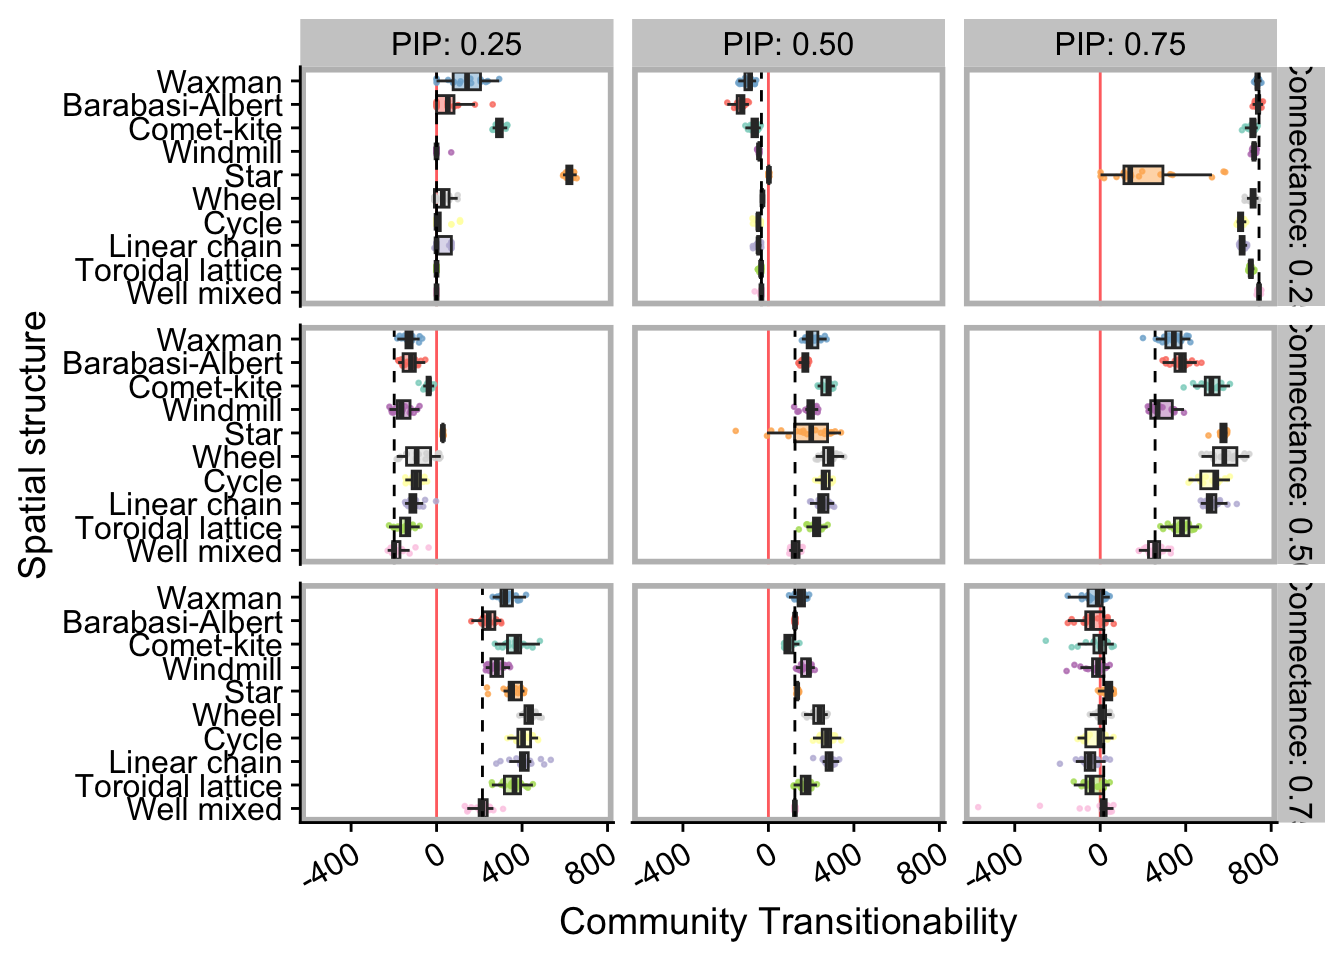
\includegraphics{supplemental-material_files/figure-latex/unnamed-chunk-9-1.pdf}

For reference, we generate a table of mean and median transitionability scores per-regime per-experiment:

\begin{Shaded}
\begin{Highlighting}[]
\NormalTok{summary\_data }\OtherTok{\textless{}{-}}\NormalTok{ rt\_final\_data }\SpecialCharTok{\%\textgreater{}\%}
\NormalTok{  dplyr}\SpecialCharTok{::}\FunctionTok{group\_by}\NormalTok{(interaction\_matrix, graph\_type) }\SpecialCharTok{\%\textgreater{}\%}
\NormalTok{  dplyr}\SpecialCharTok{::}\FunctionTok{summarize}\NormalTok{(}
    \AttributeTok{score\_median =} \FunctionTok{median}\NormalTok{(logged\_mult\_score),}
    \AttributeTok{score\_mean =} \FunctionTok{mean}\NormalTok{(logged\_mult\_score),}
    \AttributeTok{replicates =} \FunctionTok{n}\NormalTok{()}
\NormalTok{  ) }\SpecialCharTok{\%\textgreater{}\%}
  \FunctionTok{arrange}\NormalTok{(score\_median, }\AttributeTok{.by\_group =} \ConstantTok{TRUE}\NormalTok{)}

\NormalTok{summary\_table }\OtherTok{\textless{}{-}}\NormalTok{ summary\_data }\SpecialCharTok{\%\textgreater{}\%}
  \FunctionTok{kable}\NormalTok{() }\SpecialCharTok{\%\textgreater{}\%}
  \FunctionTok{kable\_styling}\NormalTok{(}
    \AttributeTok{latex\_options =} \StringTok{"striped"}
\NormalTok{  )}
\FunctionTok{save\_kable}\NormalTok{(}
\NormalTok{  summary\_table,}
  \FunctionTok{paste}\NormalTok{(}
\NormalTok{    plot\_dir,}
    \StringTok{"summary\_table.pdf"}\NormalTok{,}
    \AttributeTok{sep =} \StringTok{"/"}
\NormalTok{  )}
\NormalTok{)}
\NormalTok{summary\_table}
\end{Highlighting}
\end{Shaded}

\begin{table}
\centering
\begin{tabular}{l|l|r|r|r}
\hline
interaction\_matrix & graph\_type & score\_median & score\_mean & replicates\\
\hline
\cellcolor{gray!6}{c25pip25} & \cellcolor{gray!6}{windmill} & \cellcolor{gray!6}{-0.1552570} & \cellcolor{gray!6}{3.2755443} & \cellcolor{gray!6}{20}\\
\hline
c25pip25 & cycle & -0.1448880 & 23.2577198 & 20\\
\hline
\cellcolor{gray!6}{c25pip25} & \cellcolor{gray!6}{linear-chain} & \cellcolor{gray!6}{-0.1448875} & \cellcolor{gray!6}{30.0107428} & \cellcolor{gray!6}{20}\\
\hline
c25pip25 & toroidal-lattice & -0.1398950 & -0.1386467 & 20\\
\hline
\cellcolor{gray!6}{c25pip25} & \cellcolor{gray!6}{well-mixed} & \cellcolor{gray!6}{-0.1274125} & \cellcolor{gray!6}{-0.1274118} & \cellcolor{gray!6}{20}\\
\hline
c25pip25 & wheel & 29.1941680 & 29.2538536 & 20\\
\hline
\cellcolor{gray!6}{c25pip25} & \cellcolor{gray!6}{random-barabasi-albert} & \cellcolor{gray!6}{52.5468000} & \cellcolor{gray!6}{58.7830525} & \cellcolor{gray!6}{20}\\
\hline
c25pip25 & random-waxman & 142.6250000 & 132.2016943 & 20\\
\hline
\cellcolor{gray!6}{c25pip25} & \cellcolor{gray!6}{comet-kite} & \cellcolor{gray!6}{290.7705000} & \cellcolor{gray!6}{294.3542000} & \cellcolor{gray!6}{20}\\
\hline
c25pip25 & star & 622.3975000 & 621.4329500 & 20\\
\hline
\cellcolor{gray!6}{c25pip50} & \cellcolor{gray!6}{random-barabasi-albert} & \cellcolor{gray!6}{-123.7055000} & \cellcolor{gray!6}{-128.4367700} & \cellcolor{gray!6}{20}\\
\hline
c25pip50 & random-waxman & -85.6997500 & -93.6634050 & 20\\
\hline
\cellcolor{gray!6}{c25pip50} & \cellcolor{gray!6}{comet-kite} & \cellcolor{gray!6}{-62.4832500} & \cellcolor{gray!6}{-64.5371050} & \cellcolor{gray!6}{20}\\
\hline
c25pip50 & cycle & -46.8019500 & -48.0774750 & 20\\
\hline
\cellcolor{gray!6}{c25pip50} & \cellcolor{gray!6}{linear-chain} & \cellcolor{gray!6}{-46.2323500} & \cellcolor{gray!6}{-47.4541800} & \cellcolor{gray!6}{20}\\
\hline
c25pip50 & windmill & -44.0345500 & -44.8190350 & 20\\
\hline
\cellcolor{gray!6}{c25pip50} & \cellcolor{gray!6}{toroidal-lattice} & \cellcolor{gray!6}{-34.1670000} & \cellcolor{gray!6}{-36.9710150} & \cellcolor{gray!6}{20}\\
\hline
c25pip50 & well-mixed & -32.6162000 & -34.8772050 & 20\\
\hline
\cellcolor{gray!6}{c25pip50} & \cellcolor{gray!6}{wheel} & \cellcolor{gray!6}{-27.7729000} & \cellcolor{gray!6}{-27.7023650} & \cellcolor{gray!6}{20}\\
\hline
c25pip50 & star & 2.4022500 & 2.3551140 & 20\\
\hline
\cellcolor{gray!6}{c25pip75} & \cellcolor{gray!6}{star} & \cellcolor{gray!6}{140.4695000} & \cellcolor{gray!6}{206.2041715} & \cellcolor{gray!6}{20}\\
\hline
c25pip75 & cycle & 658.9540000 & 657.9878500 & 20\\
\hline
\cellcolor{gray!6}{c25pip75} & \cellcolor{gray!6}{linear-chain} & \cellcolor{gray!6}{664.6090000} & \cellcolor{gray!6}{665.7244000} & \cellcolor{gray!6}{20}\\
\hline
c25pip75 & toroidal-lattice & 703.8705000 & 705.6194500 & 20\\
\hline
\cellcolor{gray!6}{c25pip75} & \cellcolor{gray!6}{wheel} & \cellcolor{gray!6}{715.5445000} & \cellcolor{gray!6}{713.2512500} & \cellcolor{gray!6}{20}\\
\hline
c25pip75 & comet-kite & 717.4210000 & 711.4932000 & 20\\
\hline
\cellcolor{gray!6}{c25pip75} & \cellcolor{gray!6}{windmill} & \cellcolor{gray!6}{720.5355000} & \cellcolor{gray!6}{719.9272500} & \cellcolor{gray!6}{20}\\
\hline
c25pip75 & random-waxman & 736.0230000 & 736.1203000 & 20\\
\hline
\cellcolor{gray!6}{c25pip75} & \cellcolor{gray!6}{random-barabasi-albert} & \cellcolor{gray!6}{739.2250000} & \cellcolor{gray!6}{738.5561500} & \cellcolor{gray!6}{20}\\
\hline
c25pip75 & well-mixed & 743.1275000 & 742.8270000 & 20\\
\hline
\cellcolor{gray!6}{c50pip25} & \cellcolor{gray!6}{well-mixed} & \cellcolor{gray!6}{-198.2860000} & \cellcolor{gray!6}{-179.9309250} & \cellcolor{gray!6}{20}\\
\hline
c50pip25 & windmill & -164.2615000 & -158.1420900 & 20\\
\hline
\cellcolor{gray!6}{c50pip25} & \cellcolor{gray!6}{toroidal-lattice} & \cellcolor{gray!6}{-136.0975000} & \cellcolor{gray!6}{-146.1914300} & \cellcolor{gray!6}{20}\\
\hline
c50pip25 & random-waxman & -128.2555000 & -127.8362350 & 20\\
\hline
\cellcolor{gray!6}{c50pip25} & \cellcolor{gray!6}{random-barabasi-albert} & \cellcolor{gray!6}{-119.6675000} & \cellcolor{gray!6}{-124.3501100} & \cellcolor{gray!6}{20}\\
\hline
c50pip25 & linear-chain & -109.6645000 & -104.4384365 & 20\\
\hline
\cellcolor{gray!6}{c50pip25} & \cellcolor{gray!6}{cycle} & \cellcolor{gray!6}{-96.3967500} & \cellcolor{gray!6}{-96.4360300} & \cellcolor{gray!6}{20}\\
\hline
c50pip25 & wheel & -93.1401500 & -80.2479790 & 20\\
\hline
\cellcolor{gray!6}{c50pip25} & \cellcolor{gray!6}{comet-kite} & \cellcolor{gray!6}{-35.9154000} & \cellcolor{gray!6}{-38.5166250} & \cellcolor{gray!6}{20}\\
\hline
c50pip25 & star & 29.5336000 & 29.6897650 & 20\\
\hline
\cellcolor{gray!6}{c50pip50} & \cellcolor{gray!6}{well-mixed} & \cellcolor{gray!6}{124.5965000} & \cellcolor{gray!6}{126.7944950} & \cellcolor{gray!6}{20}\\
\hline
c50pip50 & random-barabasi-albert & 175.8165000 & 171.1758000 & 20\\
\hline
\cellcolor{gray!6}{c50pip50} & \cellcolor{gray!6}{windmill} & \cellcolor{gray!6}{195.5930000} & \cellcolor{gray!6}{192.2814000} & \cellcolor{gray!6}{20}\\
\hline
c50pip50 & random-waxman & 196.9120000 & 207.3342000 & 20\\
\hline
\cellcolor{gray!6}{c50pip50} & \cellcolor{gray!6}{star} & \cellcolor{gray!6}{200.4315000} & \cellcolor{gray!6}{179.9736390} & \cellcolor{gray!6}{20}\\
\hline
c50pip50 & toroidal-lattice & 224.4375000 & 221.0585000 & 20\\
\hline
\cellcolor{gray!6}{c50pip50} & \cellcolor{gray!6}{linear-chain} & \cellcolor{gray!6}{254.4380000} & \cellcolor{gray!6}{257.4893000} & \cellcolor{gray!6}{20}\\
\hline
c50pip50 & cycle & 260.7760000 & 265.9643500 & 20\\
\hline
\cellcolor{gray!6}{c50pip50} & \cellcolor{gray!6}{comet-kite} & \cellcolor{gray!6}{280.7530000} & \cellcolor{gray!6}{272.8958000} & \cellcolor{gray!6}{20}\\
\hline
c50pip50 & wheel & 286.9300000 & 282.9178000 & 20\\
\hline
\cellcolor{gray!6}{c50pip75} & \cellcolor{gray!6}{well-mixed} & \cellcolor{gray!6}{256.7610000} & \cellcolor{gray!6}{254.8647500} & \cellcolor{gray!6}{20}\\
\hline
c50pip75 & windmill & 268.4115000 & 284.2451000 & 20\\
\hline
\cellcolor{gray!6}{c50pip75} & \cellcolor{gray!6}{random-waxman} & \cellcolor{gray!6}{344.5975000} & \cellcolor{gray!6}{337.5601000} & \cellcolor{gray!6}{20}\\
\hline
c50pip75 & random-barabasi-albert & 378.4345000 & 376.6597000 & 20\\
\hline
\cellcolor{gray!6}{c50pip75} & \cellcolor{gray!6}{toroidal-lattice} & \cellcolor{gray!6}{382.7610000} & \cellcolor{gray!6}{377.3860000} & \cellcolor{gray!6}{20}\\
\hline
c50pip75 & linear-chain & 516.4060000 & 526.6507000 & 20\\
\hline
\cellcolor{gray!6}{c50pip75} & \cellcolor{gray!6}{comet-kite} & \cellcolor{gray!6}{520.2015000} & \cellcolor{gray!6}{517.2678500} & \cellcolor{gray!6}{20}\\
\hline
c50pip75 & cycle & 538.1730000 & 518.6681500 & 20\\
\hline
\cellcolor{gray!6}{c50pip75} & \cellcolor{gray!6}{star} & \cellcolor{gray!6}{580.5000000} & \cellcolor{gray!6}{575.3854500} & \cellcolor{gray!6}{20}\\
\hline
c50pip75 & wheel & 580.5095000 & 583.9934500 & 20\\
\hline
\cellcolor{gray!6}{c75pip25} & \cellcolor{gray!6}{well-mixed} & \cellcolor{gray!6}{214.6415000} & \cellcolor{gray!6}{213.1840000} & \cellcolor{gray!6}{20}\\
\hline
c75pip25 & random-barabasi-albert & 244.2360000 & 243.7660000 & 20\\
\hline
\cellcolor{gray!6}{c75pip25} & \cellcolor{gray!6}{windmill} & \cellcolor{gray!6}{282.1830000} & \cellcolor{gray!6}{281.7641500} & \cellcolor{gray!6}{20}\\
\hline
c75pip25 & random-waxman & 321.3525000 & 329.0571000 & 20\\
\hline
\cellcolor{gray!6}{c75pip25} & \cellcolor{gray!6}{star} & \cellcolor{gray!6}{353.5715000} & \cellcolor{gray!6}{355.4357000} & \cellcolor{gray!6}{20}\\
\hline
c75pip25 & toroidal-lattice & 364.6130000 & 358.8891000 & 20\\
\hline
\cellcolor{gray!6}{c75pip25} & \cellcolor{gray!6}{comet-kite} & \cellcolor{gray!6}{373.8350000} & \cellcolor{gray!6}{367.9652500} & \cellcolor{gray!6}{20}\\
\hline
c75pip25 & cycle & 404.5610000 & 406.7842000 & 20\\
\hline
\cellcolor{gray!6}{c75pip25} & \cellcolor{gray!6}{linear-chain} & \cellcolor{gray!6}{405.0900000} & \cellcolor{gray!6}{408.0693500} & \cellcolor{gray!6}{20}\\
\hline
c75pip25 & wheel & 433.8655000 & 434.2465500 & 20\\
\hline
\cellcolor{gray!6}{c75pip50} & \cellcolor{gray!6}{comet-kite} & \cellcolor{gray!6}{93.4602000} & \cellcolor{gray!6}{96.4563600} & \cellcolor{gray!6}{20}\\
\hline
c75pip50 & well-mixed & 123.8665000 & 123.9225000 & 20\\
\hline
\cellcolor{gray!6}{c75pip50} & \cellcolor{gray!6}{random-barabasi-albert} & \cellcolor{gray!6}{124.6680000} & \cellcolor{gray!6}{124.4696500} & \cellcolor{gray!6}{20}\\
\hline
c75pip50 & star & 134.7710000 & 135.7525500 & 20\\
\hline
\cellcolor{gray!6}{c75pip50} & \cellcolor{gray!6}{random-waxman} & \cellcolor{gray!6}{149.6610000} & \cellcolor{gray!6}{149.9015700} & \cellcolor{gray!6}{20}\\
\hline
c75pip50 & toroidal-lattice & 178.0340000 & 172.2011500 & 20\\
\hline
\cellcolor{gray!6}{c75pip50} & \cellcolor{gray!6}{windmill} & \cellcolor{gray!6}{189.2315000} & \cellcolor{gray!6}{176.3785000} & \cellcolor{gray!6}{20}\\
\hline
c75pip50 & wheel & 239.2325000 & 234.2794000 & 20\\
\hline
\cellcolor{gray!6}{c75pip50} & \cellcolor{gray!6}{cycle} & \cellcolor{gray!6}{274.0830000} & \cellcolor{gray!6}{272.9407000} & \cellcolor{gray!6}{20}\\
\hline
c75pip50 & linear-chain & 288.4625000 & 284.1089000 & 20\\
\hline
\cellcolor{gray!6}{c75pip75} & \cellcolor{gray!6}{linear-chain} & \cellcolor{gray!6}{-48.6068000} & \cellcolor{gray!6}{-48.5231200} & \cellcolor{gray!6}{20}\\
\hline
c75pip75 & toroidal-lattice & -39.6888000 & -31.2047310 & 20\\
\hline
\cellcolor{gray!6}{c75pip75} & \cellcolor{gray!6}{random-barabasi-albert} & \cellcolor{gray!6}{-38.4254000} & \cellcolor{gray!6}{-33.0213640} & \cellcolor{gray!6}{20}\\
\hline
c75pip75 & random-waxman & -11.9159500 & -24.8602700 & 20\\
\hline
\cellcolor{gray!6}{c75pip75} & \cellcolor{gray!6}{windmill} & \cellcolor{gray!6}{-10.3426000} & \cellcolor{gray!6}{-21.3472448} & \cellcolor{gray!6}{20}\\
\hline
c75pip75 & cycle & -3.3241900 & -23.7860095 & 20\\
\hline
\cellcolor{gray!6}{c75pip75} & \cellcolor{gray!6}{comet-kite} & \cellcolor{gray!6}{2.2869400} & \cellcolor{gray!6}{-17.2844405} & \cellcolor{gray!6}{20}\\
\hline
c75pip75 & wheel & 7.0713600 & 7.9136955 & 20\\
\hline
\cellcolor{gray!6}{c75pip75} & \cellcolor{gray!6}{well-mixed} & \cellcolor{gray!6}{16.4932500} & \cellcolor{gray!6}{-30.4982045} & \cellcolor{gray!6}{20}\\
\hline
c75pip75 & star & 44.9286500 & 39.1654115 & 20\\
\hline
\end{tabular}
\end{table}

\hypertarget{statistical-analyses}{%
\subsection{Statistical analyses}\label{statistical-analyses}}

\hypertarget{transitionabiliy-score-distributions---kruskal-wallis-test-results}{%
\subsubsection{Transitionabiliy score distributions - Kruskal-Wallis test results}\label{transitionabiliy-score-distributions---kruskal-wallis-test-results}}

First, a Kruskal-Wallis test (per-interaction matrix) to test for significant differences in distributions across spatial structure regimes.

\begin{Shaded}
\begin{Highlighting}[]
\NormalTok{kw\_test }\OtherTok{\textless{}{-}}\NormalTok{ rt\_final\_data }\SpecialCharTok{\%\textgreater{}\%}
  \FunctionTok{group\_by}\NormalTok{(interaction\_matrix) }\SpecialCharTok{\%\textgreater{}\%}
  \FunctionTok{kruskal\_test}\NormalTok{(logged\_mult\_score }\SpecialCharTok{\textasciitilde{}}\NormalTok{ graph\_type) }\SpecialCharTok{\%\textgreater{}\%}
  \FunctionTok{mutate}\NormalTok{(}\AttributeTok{sig =}\NormalTok{ (p }\SpecialCharTok{\textless{}} \FloatTok{0.05}\NormalTok{))}

\NormalTok{kw\_table }\OtherTok{\textless{}{-}}\NormalTok{ kw\_test }\SpecialCharTok{\%\textgreater{}\%}
  \FunctionTok{kable}\NormalTok{() }\SpecialCharTok{\%\textgreater{}\%}
  \FunctionTok{kable\_styling}\NormalTok{(}
    \AttributeTok{latex\_options =} \StringTok{"striped"}
\NormalTok{  )}
\FunctionTok{save\_kable}\NormalTok{(}
\NormalTok{  kw\_table,}
  \FunctionTok{paste}\NormalTok{(}
\NormalTok{    plot\_dir,}
    \StringTok{"kw\_test\_results.pdf"}\NormalTok{,}
    \AttributeTok{sep =} \StringTok{"/"}
\NormalTok{  )}
\NormalTok{)}
\NormalTok{kw\_table}
\end{Highlighting}
\end{Shaded}

\begin{table}
\centering
\begin{tabular}{l|l|r|r|r|r|l|l}
\hline
interaction\_matrix & .y. & n & statistic & df & p & method & sig\\
\hline
\cellcolor{gray!6}{c25pip25} & \cellcolor{gray!6}{logged\_mult\_score} & \cellcolor{gray!6}{200} & \cellcolor{gray!6}{135.4711} & \cellcolor{gray!6}{9} & \cellcolor{gray!6}{0e+00} & \cellcolor{gray!6}{Kruskal-Wallis} & \cellcolor{gray!6}{TRUE}\\
\hline
c25pip50 & logged\_mult\_score & 200 & 176.1459 & 9 & 0e+00 & Kruskal-Wallis & TRUE\\
\hline
\cellcolor{gray!6}{c25pip75} & \cellcolor{gray!6}{logged\_mult\_score} & \cellcolor{gray!6}{200} & \cellcolor{gray!6}{172.1451} & \cellcolor{gray!6}{9} & \cellcolor{gray!6}{0e+00} & \cellcolor{gray!6}{Kruskal-Wallis} & \cellcolor{gray!6}{TRUE}\\
\hline
c50pip25 & logged\_mult\_score & 200 & 128.1468 & 9 & 0e+00 & Kruskal-Wallis & TRUE\\
\hline
\cellcolor{gray!6}{c50pip50} & \cellcolor{gray!6}{logged\_mult\_score} & \cellcolor{gray!6}{200} & \cellcolor{gray!6}{125.9629} & \cellcolor{gray!6}{9} & \cellcolor{gray!6}{0e+00} & \cellcolor{gray!6}{Kruskal-Wallis} & \cellcolor{gray!6}{TRUE}\\
\hline
c50pip75 & logged\_mult\_score & 200 & 166.6052 & 9 & 0e+00 & Kruskal-Wallis & TRUE\\
\hline
\cellcolor{gray!6}{c75pip25} & \cellcolor{gray!6}{logged\_mult\_score} & \cellcolor{gray!6}{200} & \cellcolor{gray!6}{141.7244} & \cellcolor{gray!6}{9} & \cellcolor{gray!6}{0e+00} & \cellcolor{gray!6}{Kruskal-Wallis} & \cellcolor{gray!6}{TRUE}\\
\hline
c75pip50 & logged\_mult\_score & 200 & 172.4309 & 9 & 0e+00 & Kruskal-Wallis & TRUE\\
\hline
\cellcolor{gray!6}{c75pip75} & \cellcolor{gray!6}{logged\_mult\_score} & \cellcolor{gray!6}{200} & \cellcolor{gray!6}{48.4034} & \cellcolor{gray!6}{9} & \cellcolor{gray!6}{2e-07} & \cellcolor{gray!6}{Kruskal-Wallis} & \cellcolor{gray!6}{TRUE}\\
\hline
\end{tabular}
\end{table}

\hypertarget{transitionability-score-distributions---pairwise-wilcoxon-rank-sum-test-results}{%
\subsubsection{Transitionability score distributions - Pairwise Wilcoxon rank-sum test results}\label{transitionability-score-distributions---pairwise-wilcoxon-rank-sum-test-results}}

Next, we perform pairwise Wilcoxon rank-sum tests for all significant comparison groups.
We use a Holm-Bonferroni correction for multiple comparisons.

\begin{Shaded}
\begin{Highlighting}[]
\CommentTok{\# Grab group names of significant comparisons}
\NormalTok{sig\_kw\_groups }\OtherTok{\textless{}{-}} \FunctionTok{filter}\NormalTok{(kw\_test, p }\SpecialCharTok{\textless{}} \FloatTok{0.05}\NormalTok{)}\SpecialCharTok{$}\NormalTok{interaction\_matrix}
\CommentTok{\# Perform pairwise rank{-}sum tests, adjust for multiple comparisons}
\NormalTok{wrs\_test }\OtherTok{\textless{}{-}}\NormalTok{ rt\_final\_data }\SpecialCharTok{\%\textgreater{}\%}
  \FunctionTok{filter}\NormalTok{(}
\NormalTok{    interaction\_matrix }\SpecialCharTok{\%in\%}\NormalTok{ sig\_kw\_groups}
\NormalTok{  ) }\SpecialCharTok{\%\textgreater{}\%}
  \FunctionTok{group\_by}\NormalTok{(interaction\_matrix) }\SpecialCharTok{\%\textgreater{}\%}
  \FunctionTok{pairwise\_wilcox\_test}\NormalTok{(logged\_mult\_score }\SpecialCharTok{\textasciitilde{}}\NormalTok{ graph\_type) }\SpecialCharTok{\%\textgreater{}\%}
  \FunctionTok{adjust\_pvalue}\NormalTok{(}\AttributeTok{method =} \StringTok{"holm"}\NormalTok{) }\SpecialCharTok{\%\textgreater{}\%}
  \FunctionTok{add\_significance}\NormalTok{(}\StringTok{"p.adj"}\NormalTok{)}
\CommentTok{\# Build a pretty table}
\NormalTok{wrs\_test\_table }\OtherTok{\textless{}{-}} \FunctionTok{kable}\NormalTok{(wrs\_test) }\SpecialCharTok{\%\textgreater{}\%}
  \FunctionTok{kable\_styling}\NormalTok{(}
    \AttributeTok{latex\_options =} \StringTok{"striped"}
\NormalTok{  )}
\FunctionTok{save\_kable}\NormalTok{(}
\NormalTok{  wrs\_test\_table,}
  \FunctionTok{paste}\NormalTok{(}
\NormalTok{    plot\_dir,}
    \StringTok{"wrs\_test\_results.pdf"}\NormalTok{,}
    \AttributeTok{sep =} \StringTok{"/"}
\NormalTok{  )}
\NormalTok{)}
\NormalTok{wrs\_test\_table}
\end{Highlighting}
\end{Shaded}

\begin{table}
\centering
\begin{tabular}{l|l|l|l|r|r|r|r|r|l}
\hline
interaction\_matrix & .y. & group1 & group2 & n1 & n2 & statistic & p & p.adj & p.adj.signif\\
\hline
\cellcolor{gray!6}{c25pip25} & \cellcolor{gray!6}{logged\_mult\_score} & \cellcolor{gray!6}{comet-kite} & \cellcolor{gray!6}{cycle} & \cellcolor{gray!6}{20} & \cellcolor{gray!6}{20} & \cellcolor{gray!6}{400.0} & \cellcolor{gray!6}{1.00e-07} & \cellcolor{gray!6}{0.0000155} & \cellcolor{gray!6}{****}\\
\hline
c25pip25 & logged\_mult\_score & comet-kite & linear-chain & 20 & 20 & 400.0 & 1.00e-07 & 0.0000155 & ****\\
\hline
\cellcolor{gray!6}{c25pip25} & \cellcolor{gray!6}{logged\_mult\_score} & \cellcolor{gray!6}{comet-kite} & \cellcolor{gray!6}{random-barabasi-albert} & \cellcolor{gray!6}{20} & \cellcolor{gray!6}{20} & \cellcolor{gray!6}{399.0} & \cellcolor{gray!6}{1.00e-07} & \cellcolor{gray!6}{0.0000177} & \cellcolor{gray!6}{****}\\
\hline
c25pip25 & logged\_mult\_score & comet-kite & random-waxman & 20 & 20 & 388.0 & 4.00e-07 & 0.0000853 & ****\\
\hline
\cellcolor{gray!6}{c25pip25} & \cellcolor{gray!6}{logged\_mult\_score} & \cellcolor{gray!6}{comet-kite} & \cellcolor{gray!6}{star} & \cellcolor{gray!6}{20} & \cellcolor{gray!6}{20} & \cellcolor{gray!6}{0.0} & \cellcolor{gray!6}{0.00e+00} & \cellcolor{gray!6}{0.0000000} & \cellcolor{gray!6}{****}\\
\hline
c25pip25 & logged\_mult\_score & comet-kite & toroidal-lattice & 20 & 20 & 400.0 & 1.00e-07 & 0.0000148 & ****\\
\hline
\cellcolor{gray!6}{c25pip25} & \cellcolor{gray!6}{logged\_mult\_score} & \cellcolor{gray!6}{comet-kite} & \cellcolor{gray!6}{well-mixed} & \cellcolor{gray!6}{20} & \cellcolor{gray!6}{20} & \cellcolor{gray!6}{400.0} & \cellcolor{gray!6}{1.00e-07} & \cellcolor{gray!6}{0.0000151} & \cellcolor{gray!6}{****}\\
\hline
c25pip25 & logged\_mult\_score & comet-kite & wheel & 20 & 20 & 400.0 & 1.00e-07 & 0.0000155 & ****\\
\hline
\cellcolor{gray!6}{c25pip25} & \cellcolor{gray!6}{logged\_mult\_score} & \cellcolor{gray!6}{comet-kite} & \cellcolor{gray!6}{windmill} & \cellcolor{gray!6}{20} & \cellcolor{gray!6}{20} & \cellcolor{gray!6}{400.0} & \cellcolor{gray!6}{1.00e-07} & \cellcolor{gray!6}{0.0000148} & \cellcolor{gray!6}{****}\\
\hline
c25pip25 & logged\_mult\_score & cycle & linear-chain & 20 & 20 & 207.0 & 8.60e-01 & 1.0000000 & ns\\
\hline
\cellcolor{gray!6}{c25pip25} & \cellcolor{gray!6}{logged\_mult\_score} & \cellcolor{gray!6}{cycle} & \cellcolor{gray!6}{random-barabasi-albert} & \cellcolor{gray!6}{20} & \cellcolor{gray!6}{20} & \cellcolor{gray!6}{104.5} & \cellcolor{gray!6}{1.00e-02} & \cellcolor{gray!6}{1.0000000} & \cellcolor{gray!6}{ns}\\
\hline
c25pip25 & logged\_mult\_score & cycle & random-waxman & 20 & 20 & 33.0 & 6.50e-06 & 0.0011866 & **\\
\hline
\cellcolor{gray!6}{c25pip25} & \cellcolor{gray!6}{logged\_mult\_score} & \cellcolor{gray!6}{cycle} & \cellcolor{gray!6}{star} & \cellcolor{gray!6}{20} & \cellcolor{gray!6}{20} & \cellcolor{gray!6}{0.0} & \cellcolor{gray!6}{1.00e-07} & \cellcolor{gray!6}{0.0000155} & \cellcolor{gray!6}{****}\\
\hline
c25pip25 & logged\_mult\_score & cycle & toroidal-lattice & 20 & 20 & 146.5 & 1.47e-01 & 1.0000000 & ns\\
\hline
\cellcolor{gray!6}{c25pip25} & \cellcolor{gray!6}{logged\_mult\_score} & \cellcolor{gray!6}{cycle} & \cellcolor{gray!6}{well-mixed} & \cellcolor{gray!6}{20} & \cellcolor{gray!6}{20} & \cellcolor{gray!6}{105.5} & \cellcolor{gray!6}{1.10e-02} & \cellcolor{gray!6}{1.0000000} & \cellcolor{gray!6}{ns}\\
\hline
c25pip25 & logged\_mult\_score & cycle & wheel & 20 & 20 & 243.0 & 2.49e-01 & 1.0000000 & ns\\
\hline
\cellcolor{gray!6}{c25pip25} & \cellcolor{gray!6}{logged\_mult\_score} & \cellcolor{gray!6}{cycle} & \cellcolor{gray!6}{windmill} & \cellcolor{gray!6}{20} & \cellcolor{gray!6}{20} & \cellcolor{gray!6}{306.0} & \cellcolor{gray!6}{4.00e-03} & \cellcolor{gray!6}{0.5080000} & \cellcolor{gray!6}{ns}\\
\hline
c25pip25 & logged\_mult\_score & linear-chain & random-barabasi-albert & 20 & 20 & 131.5 & 6.50e-02 & 1.0000000 & ns\\
\hline
\cellcolor{gray!6}{c25pip25} & \cellcolor{gray!6}{logged\_mult\_score} & \cellcolor{gray!6}{linear-chain} & \cellcolor{gray!6}{random-waxman} & \cellcolor{gray!6}{20} & \cellcolor{gray!6}{20} & \cellcolor{gray!6}{36.0} & \cellcolor{gray!6}{9.60e-06} & \cellcolor{gray!6}{0.0016826} & \cellcolor{gray!6}{**}\\
\hline
c25pip25 & logged\_mult\_score & linear-chain & star & 20 & 20 & 0.0 & 1.00e-07 & 0.0000155 & ****\\
\hline
\cellcolor{gray!6}{c25pip25} & \cellcolor{gray!6}{logged\_mult\_score} & \cellcolor{gray!6}{linear-chain} & \cellcolor{gray!6}{toroidal-lattice} & \cellcolor{gray!6}{20} & \cellcolor{gray!6}{20} & \cellcolor{gray!6}{191.0} & \cellcolor{gray!6}{8.17e-01} & \cellcolor{gray!6}{1.0000000} & \cellcolor{gray!6}{ns}\\
\hline
c25pip25 & logged\_mult\_score & linear-chain & well-mixed & 20 & 20 & 181.0 & 6.16e-01 & 1.0000000 & ns\\
\hline
\cellcolor{gray!6}{c25pip25} & \cellcolor{gray!6}{logged\_mult\_score} & \cellcolor{gray!6}{linear-chain} & \cellcolor{gray!6}{wheel} & \cellcolor{gray!6}{20} & \cellcolor{gray!6}{20} & \cellcolor{gray!6}{256.0} & \cellcolor{gray!6}{1.32e-01} & \cellcolor{gray!6}{1.0000000} & \cellcolor{gray!6}{ns}\\
\hline
c25pip25 & logged\_mult\_score & linear-chain & windmill & 20 & 20 & 297.0 & 9.00e-03 & 1.0000000 & ns\\
\hline
\cellcolor{gray!6}{c25pip25} & \cellcolor{gray!6}{logged\_mult\_score} & \cellcolor{gray!6}{random-barabasi-albert} & \cellcolor{gray!6}{random-waxman} & \cellcolor{gray!6}{20} & \cellcolor{gray!6}{20} & \cellcolor{gray!6}{86.0} & \cellcolor{gray!6}{2.00e-03} & \cellcolor{gray!6}{0.2760000} & \cellcolor{gray!6}{ns}\\
\hline
c25pip25 & logged\_mult\_score & random-barabasi-albert & star & 20 & 20 & 0.0 & 1.00e-07 & 0.0000155 & ****\\
\hline
\cellcolor{gray!6}{c25pip25} & \cellcolor{gray!6}{logged\_mult\_score} & \cellcolor{gray!6}{random-barabasi-albert} & \cellcolor{gray!6}{toroidal-lattice} & \cellcolor{gray!6}{20} & \cellcolor{gray!6}{20} & \cellcolor{gray!6}{314.5} & \cellcolor{gray!6}{2.00e-03} & \cellcolor{gray!6}{0.2760000} & \cellcolor{gray!6}{ns}\\
\hline
c25pip25 & logged\_mult\_score & random-barabasi-albert & well-mixed & 20 & 20 & 270.5 & 5.70e-02 & 1.0000000 & ns\\
\hline
\cellcolor{gray!6}{c25pip25} & \cellcolor{gray!6}{logged\_mult\_score} & \cellcolor{gray!6}{random-barabasi-albert} & \cellcolor{gray!6}{wheel} & \cellcolor{gray!6}{20} & \cellcolor{gray!6}{20} & \cellcolor{gray!6}{256.0} & \cellcolor{gray!6}{1.33e-01} & \cellcolor{gray!6}{1.0000000} & \cellcolor{gray!6}{ns}\\
\hline
c25pip25 & logged\_mult\_score & random-barabasi-albert & windmill & 20 & 20 & 374.0 & 2.50e-06 & 0.0004806 & ***\\
\hline
\cellcolor{gray!6}{c25pip25} & \cellcolor{gray!6}{logged\_mult\_score} & \cellcolor{gray!6}{random-waxman} & \cellcolor{gray!6}{star} & \cellcolor{gray!6}{20} & \cellcolor{gray!6}{20} & \cellcolor{gray!6}{0.0} & \cellcolor{gray!6}{1.00e-07} & \cellcolor{gray!6}{0.0000155} & \cellcolor{gray!6}{****}\\
\hline
c25pip25 & logged\_mult\_score & random-waxman & toroidal-lattice & 20 & 20 & 385.5 & 5.00e-07 & 0.0001071 & ***\\
\hline
\cellcolor{gray!6}{c25pip25} & \cellcolor{gray!6}{logged\_mult\_score} & \cellcolor{gray!6}{random-waxman} & \cellcolor{gray!6}{well-mixed} & \cellcolor{gray!6}{20} & \cellcolor{gray!6}{20} & \cellcolor{gray!6}{354.5} & \cellcolor{gray!6}{2.91e-05} & \cellcolor{gray!6}{0.0048430} & \cellcolor{gray!6}{**}\\
\hline
c25pip25 & logged\_mult\_score & random-waxman & wheel & 20 & 20 & 354.0 & 3.25e-05 & 0.0053625 & **\\
\hline
\cellcolor{gray!6}{c25pip25} & \cellcolor{gray!6}{logged\_mult\_score} & \cellcolor{gray!6}{random-waxman} & \cellcolor{gray!6}{windmill} & \cellcolor{gray!6}{20} & \cellcolor{gray!6}{20} & \cellcolor{gray!6}{396.0} & \cellcolor{gray!6}{1.00e-07} & \cellcolor{gray!6}{0.0000253} & \cellcolor{gray!6}{****}\\
\hline
c25pip25 & logged\_mult\_score & star & toroidal-lattice & 20 & 20 & 400.0 & 1.00e-07 & 0.0000148 & ****\\
\hline
\cellcolor{gray!6}{c25pip25} & \cellcolor{gray!6}{logged\_mult\_score} & \cellcolor{gray!6}{star} & \cellcolor{gray!6}{well-mixed} & \cellcolor{gray!6}{20} & \cellcolor{gray!6}{20} & \cellcolor{gray!6}{400.0} & \cellcolor{gray!6}{1.00e-07} & \cellcolor{gray!6}{0.0000151} & \cellcolor{gray!6}{****}\\
\hline
c25pip25 & logged\_mult\_score & star & wheel & 20 & 20 & 400.0 & 1.00e-07 & 0.0000155 & ****\\
\hline
\cellcolor{gray!6}{c25pip25} & \cellcolor{gray!6}{logged\_mult\_score} & \cellcolor{gray!6}{star} & \cellcolor{gray!6}{windmill} & \cellcolor{gray!6}{20} & \cellcolor{gray!6}{20} & \cellcolor{gray!6}{400.0} & \cellcolor{gray!6}{1.00e-07} & \cellcolor{gray!6}{0.0000148} & \cellcolor{gray!6}{****}\\
\hline
c25pip25 & logged\_mult\_score & toroidal-lattice & well-mixed & 20 & 20 & 53.5 & 6.37e-05 & 0.0101920 & *\\
\hline
\cellcolor{gray!6}{c25pip25} & \cellcolor{gray!6}{logged\_mult\_score} & \cellcolor{gray!6}{toroidal-lattice} & \cellcolor{gray!6}{wheel} & \cellcolor{gray!6}{20} & \cellcolor{gray!6}{20} & \cellcolor{gray!6}{200.0} & \cellcolor{gray!6}{1.00e+00} & \cellcolor{gray!6}{1.0000000} & \cellcolor{gray!6}{ns}\\
\hline
c25pip25 & logged\_mult\_score & toroidal-lattice & windmill & 20 & 20 & 357.0 & 2.04e-05 & 0.0034476 & **\\
\hline
\cellcolor{gray!6}{c25pip25} & \cellcolor{gray!6}{logged\_mult\_score} & \cellcolor{gray!6}{well-mixed} & \cellcolor{gray!6}{wheel} & \cellcolor{gray!6}{20} & \cellcolor{gray!6}{20} & \cellcolor{gray!6}{200.0} & \cellcolor{gray!6}{1.00e+00} & \cellcolor{gray!6}{1.0000000} & \cellcolor{gray!6}{ns}\\
\hline
c25pip25 & logged\_mult\_score & well-mixed & windmill & 20 & 20 & 378.0 & 1.40e-06 & 0.0002808 & ***\\
\hline
\cellcolor{gray!6}{c25pip25} & \cellcolor{gray!6}{logged\_mult\_score} & \cellcolor{gray!6}{wheel} & \cellcolor{gray!6}{windmill} & \cellcolor{gray!6}{20} & \cellcolor{gray!6}{20} & \cellcolor{gray!6}{206.0} & \cellcolor{gray!6}{8.81e-01} & \cellcolor{gray!6}{1.0000000} & \cellcolor{gray!6}{ns}\\
\hline
c25pip50 & logged\_mult\_score & comet-kite & cycle & 20 & 20 & 89.0 & 2.00e-03 & 0.2760000 & ns\\
\hline
\cellcolor{gray!6}{c25pip50} & \cellcolor{gray!6}{logged\_mult\_score} & \cellcolor{gray!6}{comet-kite} & \cellcolor{gray!6}{linear-chain} & \cellcolor{gray!6}{20} & \cellcolor{gray!6}{20} & \cellcolor{gray!6}{83.0} & \cellcolor{gray!6}{1.00e-03} & \cellcolor{gray!6}{0.1430000} & \cellcolor{gray!6}{ns}\\
\hline
c25pip50 & logged\_mult\_score & comet-kite & random-barabasi-albert & 20 & 20 & 396.0 & 0.00e+00 & 0.0000000 & ****\\
\hline
\cellcolor{gray!6}{c25pip50} & \cellcolor{gray!6}{logged\_mult\_score} & \cellcolor{gray!6}{comet-kite} & \cellcolor{gray!6}{random-waxman} & \cellcolor{gray!6}{20} & \cellcolor{gray!6}{20} & \cellcolor{gray!6}{340.0} & \cellcolor{gray!6}{6.91e-05} & \cellcolor{gray!6}{0.0109869} & \cellcolor{gray!6}{*}\\
\hline
c25pip50 & logged\_mult\_score & comet-kite & star & 20 & 20 & 0.0 & 0.00e+00 & 0.0000000 & ****\\
\hline
\cellcolor{gray!6}{c25pip50} & \cellcolor{gray!6}{logged\_mult\_score} & \cellcolor{gray!6}{comet-kite} & \cellcolor{gray!6}{toroidal-lattice} & \cellcolor{gray!6}{20} & \cellcolor{gray!6}{20} & \cellcolor{gray!6}{17.0} & \cellcolor{gray!6}{0.00e+00} & \cellcolor{gray!6}{0.0000044} & \cellcolor{gray!6}{****}\\
\hline
c25pip50 & logged\_mult\_score & comet-kite & well-mixed & 20 & 20 & 14.0 & 0.00e+00 & 0.0000019 & ****\\
\hline
\cellcolor{gray!6}{c25pip50} & \cellcolor{gray!6}{logged\_mult\_score} & \cellcolor{gray!6}{comet-kite} & \cellcolor{gray!6}{wheel} & \cellcolor{gray!6}{20} & \cellcolor{gray!6}{20} & \cellcolor{gray!6}{0.0} & \cellcolor{gray!6}{0.00e+00} & \cellcolor{gray!6}{0.0000000} & \cellcolor{gray!6}{****}\\
\hline
c25pip50 & logged\_mult\_score & comet-kite & windmill & 20 & 20 & 65.0 & 1.36e-04 & 0.0209440 & *\\
\hline
\cellcolor{gray!6}{c25pip50} & \cellcolor{gray!6}{logged\_mult\_score} & \cellcolor{gray!6}{cycle} & \cellcolor{gray!6}{linear-chain} & \cellcolor{gray!6}{20} & \cellcolor{gray!6}{20} & \cellcolor{gray!6}{176.0} & \cellcolor{gray!6}{5.29e-01} & \cellcolor{gray!6}{1.0000000} & \cellcolor{gray!6}{ns}\\
\hline
c25pip50 & logged\_mult\_score & cycle & random-barabasi-albert & 20 & 20 & 400.0 & 0.00e+00 & 0.0000000 & ****\\
\hline
\cellcolor{gray!6}{c25pip50} & \cellcolor{gray!6}{logged\_mult\_score} & \cellcolor{gray!6}{cycle} & \cellcolor{gray!6}{random-waxman} & \cellcolor{gray!6}{20} & \cellcolor{gray!6}{20} & \cellcolor{gray!6}{392.0} & \cellcolor{gray!6}{0.00e+00} & \cellcolor{gray!6}{0.0000003} & \cellcolor{gray!6}{****}\\
\hline
c25pip50 & logged\_mult\_score & cycle & star & 20 & 20 & 0.0 & 0.00e+00 & 0.0000000 & ****\\
\hline
\cellcolor{gray!6}{c25pip50} & \cellcolor{gray!6}{logged\_mult\_score} & \cellcolor{gray!6}{cycle} & \cellcolor{gray!6}{toroidal-lattice} & \cellcolor{gray!6}{20} & \cellcolor{gray!6}{20} & \cellcolor{gray!6}{45.0} & \cellcolor{gray!6}{6.90e-06} & \cellcolor{gray!6}{0.0012507} & \cellcolor{gray!6}{**}\\
\hline
c25pip50 & logged\_mult\_score & cycle & well-mixed & 20 & 20 & 28.0 & 3.00e-07 & 0.0000578 & ****\\
\hline
\cellcolor{gray!6}{c25pip50} & \cellcolor{gray!6}{logged\_mult\_score} & \cellcolor{gray!6}{cycle} & \cellcolor{gray!6}{wheel} & \cellcolor{gray!6}{20} & \cellcolor{gray!6}{20} & \cellcolor{gray!6}{0.0} & \cellcolor{gray!6}{0.00e+00} & \cellcolor{gray!6}{0.0000000} & \cellcolor{gray!6}{****}\\
\hline
c25pip50 & logged\_mult\_score & cycle & windmill & 20 & 20 & 194.0 & 8.83e-01 & 1.0000000 & ns\\
\hline
\cellcolor{gray!6}{c25pip50} & \cellcolor{gray!6}{logged\_mult\_score} & \cellcolor{gray!6}{linear-chain} & \cellcolor{gray!6}{random-barabasi-albert} & \cellcolor{gray!6}{20} & \cellcolor{gray!6}{20} & \cellcolor{gray!6}{400.0} & \cellcolor{gray!6}{0.00e+00} & \cellcolor{gray!6}{0.0000000} & \cellcolor{gray!6}{****}\\
\hline
c25pip50 & logged\_mult\_score & linear-chain & random-waxman & 20 & 20 & 392.0 & 0.00e+00 & 0.0000003 & ****\\
\hline
\cellcolor{gray!6}{c25pip50} & \cellcolor{gray!6}{logged\_mult\_score} & \cellcolor{gray!6}{linear-chain} & \cellcolor{gray!6}{star} & \cellcolor{gray!6}{20} & \cellcolor{gray!6}{20} & \cellcolor{gray!6}{0.0} & \cellcolor{gray!6}{0.00e+00} & \cellcolor{gray!6}{0.0000000} & \cellcolor{gray!6}{****}\\
\hline
c25pip50 & logged\_mult\_score & linear-chain & toroidal-lattice & 20 & 20 & 67.0 & 1.77e-04 & 0.0269040 & *\\
\hline
\cellcolor{gray!6}{c25pip50} & \cellcolor{gray!6}{logged\_mult\_score} & \cellcolor{gray!6}{linear-chain} & \cellcolor{gray!6}{well-mixed} & \cellcolor{gray!6}{20} & \cellcolor{gray!6}{20} & \cellcolor{gray!6}{32.0} & \cellcolor{gray!6}{6.00e-07} & \cellcolor{gray!6}{0.0001329} & \cellcolor{gray!6}{***}\\
\hline
c25pip50 & logged\_mult\_score & linear-chain & wheel & 20 & 20 & 0.0 & 0.00e+00 & 0.0000000 & ****\\
\hline
\cellcolor{gray!6}{c25pip50} & \cellcolor{gray!6}{logged\_mult\_score} & \cellcolor{gray!6}{linear-chain} & \cellcolor{gray!6}{windmill} & \cellcolor{gray!6}{20} & \cellcolor{gray!6}{20} & \cellcolor{gray!6}{202.0} & \cellcolor{gray!6}{9.68e-01} & \cellcolor{gray!6}{1.0000000} & \cellcolor{gray!6}{ns}\\
\hline
c25pip50 & logged\_mult\_score & random-barabasi-albert & random-waxman & 20 & 20 & 62.0 & 9.10e-05 & 0.0141960 & *\\
\hline
\cellcolor{gray!6}{c25pip50} & \cellcolor{gray!6}{logged\_mult\_score} & \cellcolor{gray!6}{random-barabasi-albert} & \cellcolor{gray!6}{star} & \cellcolor{gray!6}{20} & \cellcolor{gray!6}{20} & \cellcolor{gray!6}{0.0} & \cellcolor{gray!6}{0.00e+00} & \cellcolor{gray!6}{0.0000000} & \cellcolor{gray!6}{****}\\
\hline
c25pip50 & logged\_mult\_score & random-barabasi-albert & toroidal-lattice & 20 & 20 & 0.0 & 0.00e+00 & 0.0000000 & ****\\
\hline
\cellcolor{gray!6}{c25pip50} & \cellcolor{gray!6}{logged\_mult\_score} & \cellcolor{gray!6}{random-barabasi-albert} & \cellcolor{gray!6}{well-mixed} & \cellcolor{gray!6}{20} & \cellcolor{gray!6}{20} & \cellcolor{gray!6}{0.0} & \cellcolor{gray!6}{0.00e+00} & \cellcolor{gray!6}{0.0000000} & \cellcolor{gray!6}{****}\\
\hline
c25pip50 & logged\_mult\_score & random-barabasi-albert & wheel & 20 & 20 & 0.0 & 0.00e+00 & 0.0000000 & ****\\
\hline
\cellcolor{gray!6}{c25pip50} & \cellcolor{gray!6}{logged\_mult\_score} & \cellcolor{gray!6}{random-barabasi-albert} & \cellcolor{gray!6}{windmill} & \cellcolor{gray!6}{20} & \cellcolor{gray!6}{20} & \cellcolor{gray!6}{0.0} & \cellcolor{gray!6}{0.00e+00} & \cellcolor{gray!6}{0.0000000} & \cellcolor{gray!6}{****}\\
\hline
c25pip50 & logged\_mult\_score & random-waxman & star & 20 & 20 & 0.0 & 0.00e+00 & 0.0000000 & ****\\
\hline
\cellcolor{gray!6}{c25pip50} & \cellcolor{gray!6}{logged\_mult\_score} & \cellcolor{gray!6}{random-waxman} & \cellcolor{gray!6}{toroidal-lattice} & \cellcolor{gray!6}{20} & \cellcolor{gray!6}{20} & \cellcolor{gray!6}{0.0} & \cellcolor{gray!6}{0.00e+00} & \cellcolor{gray!6}{0.0000000} & \cellcolor{gray!6}{****}\\
\hline
c25pip50 & logged\_mult\_score & random-waxman & well-mixed & 20 & 20 & 3.0 & 0.00e+00 & 0.0000000 & ****\\
\hline
\cellcolor{gray!6}{c25pip50} & \cellcolor{gray!6}{logged\_mult\_score} & \cellcolor{gray!6}{random-waxman} & \cellcolor{gray!6}{wheel} & \cellcolor{gray!6}{20} & \cellcolor{gray!6}{20} & \cellcolor{gray!6}{0.0} & \cellcolor{gray!6}{0.00e+00} & \cellcolor{gray!6}{0.0000000} & \cellcolor{gray!6}{****}\\
\hline
c25pip50 & logged\_mult\_score & random-waxman & windmill & 20 & 20 & 0.0 & 0.00e+00 & 0.0000000 & ****\\
\hline
\cellcolor{gray!6}{c25pip50} & \cellcolor{gray!6}{logged\_mult\_score} & \cellcolor{gray!6}{star} & \cellcolor{gray!6}{toroidal-lattice} & \cellcolor{gray!6}{20} & \cellcolor{gray!6}{20} & \cellcolor{gray!6}{400.0} & \cellcolor{gray!6}{0.00e+00} & \cellcolor{gray!6}{0.0000000} & \cellcolor{gray!6}{****}\\
\hline
c25pip50 & logged\_mult\_score & star & well-mixed & 20 & 20 & 400.0 & 0.00e+00 & 0.0000000 & ****\\
\hline
\cellcolor{gray!6}{c25pip50} & \cellcolor{gray!6}{logged\_mult\_score} & \cellcolor{gray!6}{star} & \cellcolor{gray!6}{wheel} & \cellcolor{gray!6}{20} & \cellcolor{gray!6}{20} & \cellcolor{gray!6}{400.0} & \cellcolor{gray!6}{0.00e+00} & \cellcolor{gray!6}{0.0000000} & \cellcolor{gray!6}{****}\\
\hline
c25pip50 & logged\_mult\_score & star & windmill & 20 & 20 & 400.0 & 0.00e+00 & 0.0000000 & ****\\
\hline
\cellcolor{gray!6}{c25pip50} & \cellcolor{gray!6}{logged\_mult\_score} & \cellcolor{gray!6}{toroidal-lattice} & \cellcolor{gray!6}{well-mixed} & \cellcolor{gray!6}{20} & \cellcolor{gray!6}{20} & \cellcolor{gray!6}{82.0} & \cellcolor{gray!6}{1.00e-03} & \cellcolor{gray!6}{0.1430000} & \cellcolor{gray!6}{ns}\\
\hline
c25pip50 & logged\_mult\_score & toroidal-lattice & wheel & 20 & 20 & 0.0 & 0.00e+00 & 0.0000000 & ****\\
\hline
\cellcolor{gray!6}{c25pip50} & \cellcolor{gray!6}{logged\_mult\_score} & \cellcolor{gray!6}{toroidal-lattice} & \cellcolor{gray!6}{windmill} & \cellcolor{gray!6}{20} & \cellcolor{gray!6}{20} & \cellcolor{gray!6}{345.0} & \cellcolor{gray!6}{3.36e-05} & \cellcolor{gray!6}{0.0055104} & \cellcolor{gray!6}{**}\\
\hline
c25pip50 & logged\_mult\_score & well-mixed & wheel & 20 & 20 & 0.0 & 0.00e+00 & 0.0000000 & ****\\
\hline
\cellcolor{gray!6}{c25pip50} & \cellcolor{gray!6}{logged\_mult\_score} & \cellcolor{gray!6}{well-mixed} & \cellcolor{gray!6}{windmill} & \cellcolor{gray!6}{20} & \cellcolor{gray!6}{20} & \cellcolor{gray!6}{380.0} & \cellcolor{gray!6}{0.00e+00} & \cellcolor{gray!6}{0.0000097} & \cellcolor{gray!6}{****}\\
\hline
c25pip50 & logged\_mult\_score & wheel & windmill & 20 & 20 & 400.0 & 0.00e+00 & 0.0000000 & ****\\
\hline
\cellcolor{gray!6}{c25pip75} & \cellcolor{gray!6}{logged\_mult\_score} & \cellcolor{gray!6}{comet-kite} & \cellcolor{gray!6}{cycle} & \cellcolor{gray!6}{20} & \cellcolor{gray!6}{20} & \cellcolor{gray!6}{390.0} & \cellcolor{gray!6}{0.00e+00} & \cellcolor{gray!6}{0.0000005} & \cellcolor{gray!6}{****}\\
\hline
c25pip75 & logged\_mult\_score & comet-kite & linear-chain & 20 & 20 & 384.0 & 0.00e+00 & 0.0000034 & ****\\
\hline
\cellcolor{gray!6}{c25pip75} & \cellcolor{gray!6}{logged\_mult\_score} & \cellcolor{gray!6}{comet-kite} & \cellcolor{gray!6}{random-barabasi-albert} & \cellcolor{gray!6}{20} & \cellcolor{gray!6}{20} & \cellcolor{gray!6}{33.0} & \cellcolor{gray!6}{8.00e-07} & \cellcolor{gray!6}{0.0001597} & \cellcolor{gray!6}{***}\\
\hline
c25pip75 & logged\_mult\_score & comet-kite & random-waxman & 20 & 20 & 32.0 & 6.00e-07 & 0.0001329 & ***\\
\hline
\cellcolor{gray!6}{c25pip75} & \cellcolor{gray!6}{logged\_mult\_score} & \cellcolor{gray!6}{comet-kite} & \cellcolor{gray!6}{star} & \cellcolor{gray!6}{20} & \cellcolor{gray!6}{20} & \cellcolor{gray!6}{400.0} & \cellcolor{gray!6}{0.00e+00} & \cellcolor{gray!6}{0.0000000} & \cellcolor{gray!6}{****}\\
\hline
c25pip75 & logged\_mult\_score & comet-kite & toroidal-lattice & 20 & 20 & 274.0 & 4.60e-02 & 1.0000000 & ns\\
\hline
\cellcolor{gray!6}{c25pip75} & \cellcolor{gray!6}{logged\_mult\_score} & \cellcolor{gray!6}{comet-kite} & \cellcolor{gray!6}{well-mixed} & \cellcolor{gray!6}{20} & \cellcolor{gray!6}{20} & \cellcolor{gray!6}{2.0} & \cellcolor{gray!6}{0.00e+00} & \cellcolor{gray!6}{0.0000000} & \cellcolor{gray!6}{****}\\
\hline
c25pip75 & logged\_mult\_score & comet-kite & wheel & 20 & 20 & 196.0 & 9.25e-01 & 1.0000000 & ns\\
\hline
\cellcolor{gray!6}{c25pip75} & \cellcolor{gray!6}{logged\_mult\_score} & \cellcolor{gray!6}{comet-kite} & \cellcolor{gray!6}{windmill} & \cellcolor{gray!6}{20} & \cellcolor{gray!6}{20} & \cellcolor{gray!6}{159.0} & \cellcolor{gray!6}{2.77e-01} & \cellcolor{gray!6}{1.0000000} & \cellcolor{gray!6}{ns}\\
\hline
c25pip75 & logged\_mult\_score & cycle & linear-chain & 20 & 20 & 134.0 & 7.60e-02 & 1.0000000 & ns\\
\hline
\cellcolor{gray!6}{c25pip75} & \cellcolor{gray!6}{logged\_mult\_score} & \cellcolor{gray!6}{cycle} & \cellcolor{gray!6}{random-barabasi-albert} & \cellcolor{gray!6}{20} & \cellcolor{gray!6}{20} & \cellcolor{gray!6}{0.0} & \cellcolor{gray!6}{0.00e+00} & \cellcolor{gray!6}{0.0000000} & \cellcolor{gray!6}{****}\\
\hline
c25pip75 & logged\_mult\_score & cycle & random-waxman & 20 & 20 & 0.0 & 0.00e+00 & 0.0000000 & ****\\
\hline
\cellcolor{gray!6}{c25pip75} & \cellcolor{gray!6}{logged\_mult\_score} & \cellcolor{gray!6}{cycle} & \cellcolor{gray!6}{star} & \cellcolor{gray!6}{20} & \cellcolor{gray!6}{20} & \cellcolor{gray!6}{400.0} & \cellcolor{gray!6}{0.00e+00} & \cellcolor{gray!6}{0.0000000} & \cellcolor{gray!6}{****}\\
\hline
c25pip75 & logged\_mult\_score & cycle & toroidal-lattice & 20 & 20 & 0.0 & 0.00e+00 & 0.0000000 & ****\\
\hline
\cellcolor{gray!6}{c25pip75} & \cellcolor{gray!6}{logged\_mult\_score} & \cellcolor{gray!6}{cycle} & \cellcolor{gray!6}{well-mixed} & \cellcolor{gray!6}{20} & \cellcolor{gray!6}{20} & \cellcolor{gray!6}{0.0} & \cellcolor{gray!6}{0.00e+00} & \cellcolor{gray!6}{0.0000000} & \cellcolor{gray!6}{****}\\
\hline
c25pip75 & logged\_mult\_score & cycle & wheel & 20 & 20 & 2.0 & 0.00e+00 & 0.0000000 & ****\\
\hline
\cellcolor{gray!6}{c25pip75} & \cellcolor{gray!6}{logged\_mult\_score} & \cellcolor{gray!6}{cycle} & \cellcolor{gray!6}{windmill} & \cellcolor{gray!6}{20} & \cellcolor{gray!6}{20} & \cellcolor{gray!6}{0.0} & \cellcolor{gray!6}{0.00e+00} & \cellcolor{gray!6}{0.0000000} & \cellcolor{gray!6}{****}\\
\hline
c25pip75 & logged\_mult\_score & linear-chain & random-barabasi-albert & 20 & 20 & 0.0 & 0.00e+00 & 0.0000000 & ****\\
\hline
\cellcolor{gray!6}{c25pip75} & \cellcolor{gray!6}{logged\_mult\_score} & \cellcolor{gray!6}{linear-chain} & \cellcolor{gray!6}{random-waxman} & \cellcolor{gray!6}{20} & \cellcolor{gray!6}{20} & \cellcolor{gray!6}{0.0} & \cellcolor{gray!6}{0.00e+00} & \cellcolor{gray!6}{0.0000000} & \cellcolor{gray!6}{****}\\
\hline
c25pip75 & logged\_mult\_score & linear-chain & star & 20 & 20 & 400.0 & 0.00e+00 & 0.0000000 & ****\\
\hline
\cellcolor{gray!6}{c25pip75} & \cellcolor{gray!6}{logged\_mult\_score} & \cellcolor{gray!6}{linear-chain} & \cellcolor{gray!6}{toroidal-lattice} & \cellcolor{gray!6}{20} & \cellcolor{gray!6}{20} & \cellcolor{gray!6}{0.0} & \cellcolor{gray!6}{0.00e+00} & \cellcolor{gray!6}{0.0000000} & \cellcolor{gray!6}{****}\\
\hline
c25pip75 & logged\_mult\_score & linear-chain & well-mixed & 20 & 20 & 0.0 & 0.00e+00 & 0.0000000 & ****\\
\hline
\cellcolor{gray!6}{c25pip75} & \cellcolor{gray!6}{logged\_mult\_score} & \cellcolor{gray!6}{linear-chain} & \cellcolor{gray!6}{wheel} & \cellcolor{gray!6}{20} & \cellcolor{gray!6}{20} & \cellcolor{gray!6}{9.0} & \cellcolor{gray!6}{0.00e+00} & \cellcolor{gray!6}{0.0000004} & \cellcolor{gray!6}{****}\\
\hline
c25pip75 & logged\_mult\_score & linear-chain & windmill & 20 & 20 & 0.0 & 0.00e+00 & 0.0000000 & ****\\
\hline
\cellcolor{gray!6}{c25pip75} & \cellcolor{gray!6}{logged\_mult\_score} & \cellcolor{gray!6}{random-barabasi-albert} & \cellcolor{gray!6}{random-waxman} & \cellcolor{gray!6}{20} & \cellcolor{gray!6}{20} & \cellcolor{gray!6}{230.0} & \cellcolor{gray!6}{4.29e-01} & \cellcolor{gray!6}{1.0000000} & \cellcolor{gray!6}{ns}\\
\hline
c25pip75 & logged\_mult\_score & random-barabasi-albert & star & 20 & 20 & 400.0 & 0.00e+00 & 0.0000000 & ****\\
\hline
\cellcolor{gray!6}{c25pip75} & \cellcolor{gray!6}{logged\_mult\_score} & \cellcolor{gray!6}{random-barabasi-albert} & \cellcolor{gray!6}{toroidal-lattice} & \cellcolor{gray!6}{20} & \cellcolor{gray!6}{20} & \cellcolor{gray!6}{395.0} & \cellcolor{gray!6}{0.00e+00} & \cellcolor{gray!6}{0.0000001} & \cellcolor{gray!6}{****}\\
\hline
c25pip75 & logged\_mult\_score & random-barabasi-albert & well-mixed & 20 & 20 & 159.0 & 2.77e-01 & 1.0000000 & ns\\
\hline
\cellcolor{gray!6}{c25pip75} & \cellcolor{gray!6}{logged\_mult\_score} & \cellcolor{gray!6}{random-barabasi-albert} & \cellcolor{gray!6}{wheel} & \cellcolor{gray!6}{20} & \cellcolor{gray!6}{20} & \cellcolor{gray!6}{355.0} & \cellcolor{gray!6}{6.90e-06} & \cellcolor{gray!6}{0.0012507} & \cellcolor{gray!6}{**}\\
\hline
c25pip75 & logged\_mult\_score & random-barabasi-albert & windmill & 20 & 20 & 359.0 & 3.40e-06 & 0.0006486 & ***\\
\hline
\cellcolor{gray!6}{c25pip75} & \cellcolor{gray!6}{logged\_mult\_score} & \cellcolor{gray!6}{random-waxman} & \cellcolor{gray!6}{star} & \cellcolor{gray!6}{20} & \cellcolor{gray!6}{20} & \cellcolor{gray!6}{400.0} & \cellcolor{gray!6}{0.00e+00} & \cellcolor{gray!6}{0.0000000} & \cellcolor{gray!6}{****}\\
\hline
c25pip75 & logged\_mult\_score & random-waxman & toroidal-lattice & 20 & 20 & 398.0 & 0.00e+00 & 0.0000000 & ****\\
\hline
\cellcolor{gray!6}{c25pip75} & \cellcolor{gray!6}{logged\_mult\_score} & \cellcolor{gray!6}{random-waxman} & \cellcolor{gray!6}{well-mixed} & \cellcolor{gray!6}{20} & \cellcolor{gray!6}{20} & \cellcolor{gray!6}{95.0} & \cellcolor{gray!6}{4.00e-03} & \cellcolor{gray!6}{0.5080000} & \cellcolor{gray!6}{ns}\\
\hline
c25pip75 & logged\_mult\_score & random-waxman & wheel & 20 & 20 & 361.0 & 2.40e-06 & 0.0004656 & ***\\
\hline
\cellcolor{gray!6}{c25pip75} & \cellcolor{gray!6}{logged\_mult\_score} & \cellcolor{gray!6}{random-waxman} & \cellcolor{gray!6}{windmill} & \cellcolor{gray!6}{20} & \cellcolor{gray!6}{20} & \cellcolor{gray!6}{368.0} & \cellcolor{gray!6}{6.00e-07} & \cellcolor{gray!6}{0.0001329} & \cellcolor{gray!6}{***}\\
\hline
c25pip75 & logged\_mult\_score & star & toroidal-lattice & 20 & 20 & 0.0 & 0.00e+00 & 0.0000000 & ****\\
\hline
\cellcolor{gray!6}{c25pip75} & \cellcolor{gray!6}{logged\_mult\_score} & \cellcolor{gray!6}{star} & \cellcolor{gray!6}{well-mixed} & \cellcolor{gray!6}{20} & \cellcolor{gray!6}{20} & \cellcolor{gray!6}{0.0} & \cellcolor{gray!6}{0.00e+00} & \cellcolor{gray!6}{0.0000000} & \cellcolor{gray!6}{****}\\
\hline
c25pip75 & logged\_mult\_score & star & wheel & 20 & 20 & 0.0 & 0.00e+00 & 0.0000000 & ****\\
\hline
\cellcolor{gray!6}{c25pip75} & \cellcolor{gray!6}{logged\_mult\_score} & \cellcolor{gray!6}{star} & \cellcolor{gray!6}{windmill} & \cellcolor{gray!6}{20} & \cellcolor{gray!6}{20} & \cellcolor{gray!6}{0.0} & \cellcolor{gray!6}{0.00e+00} & \cellcolor{gray!6}{0.0000000} & \cellcolor{gray!6}{****}\\
\hline
c25pip75 & logged\_mult\_score & toroidal-lattice & well-mixed & 20 & 20 & 0.0 & 0.00e+00 & 0.0000000 & ****\\
\hline
\cellcolor{gray!6}{c25pip75} & \cellcolor{gray!6}{logged\_mult\_score} & \cellcolor{gray!6}{toroidal-lattice} & \cellcolor{gray!6}{wheel} & \cellcolor{gray!6}{20} & \cellcolor{gray!6}{20} & \cellcolor{gray!6}{120.0} & \cellcolor{gray!6}{3.00e-02} & \cellcolor{gray!6}{1.0000000} & \cellcolor{gray!6}{ns}\\
\hline
c25pip75 & logged\_mult\_score & toroidal-lattice & windmill & 20 & 20 & 47.0 & 9.70e-06 & 0.0016888 & **\\
\hline
\cellcolor{gray!6}{c25pip75} & \cellcolor{gray!6}{logged\_mult\_score} & \cellcolor{gray!6}{well-mixed} & \cellcolor{gray!6}{wheel} & \cellcolor{gray!6}{20} & \cellcolor{gray!6}{20} & \cellcolor{gray!6}{387.0} & \cellcolor{gray!6}{0.00e+00} & \cellcolor{gray!6}{0.0000014} & \cellcolor{gray!6}{****}\\
\hline
c25pip75 & logged\_mult\_score & well-mixed & windmill & 20 & 20 & 399.0 & 0.00e+00 & 0.0000000 & ****\\
\hline
\cellcolor{gray!6}{c25pip75} & \cellcolor{gray!6}{logged\_mult\_score} & \cellcolor{gray!6}{wheel} & \cellcolor{gray!6}{windmill} & \cellcolor{gray!6}{20} & \cellcolor{gray!6}{20} & \cellcolor{gray!6}{166.0} & \cellcolor{gray!6}{3.69e-01} & \cellcolor{gray!6}{1.0000000} & \cellcolor{gray!6}{ns}\\
\hline
c50pip25 & logged\_mult\_score & comet-kite & cycle & 20 & 20 & 386.0 & 0.00e+00 & 0.0000019 & ****\\
\hline
\cellcolor{gray!6}{c50pip25} & \cellcolor{gray!6}{logged\_mult\_score} & \cellcolor{gray!6}{comet-kite} & \cellcolor{gray!6}{linear-chain} & \cellcolor{gray!6}{20} & \cellcolor{gray!6}{20} & \cellcolor{gray!6}{375.0} & \cellcolor{gray!6}{1.00e-07} & \cellcolor{gray!6}{0.0000299} & \cellcolor{gray!6}{****}\\
\hline
c50pip25 & logged\_mult\_score & comet-kite & random-barabasi-albert & 20 & 20 & 396.0 & 0.00e+00 & 0.0000000 & ****\\
\hline
\cellcolor{gray!6}{c50pip25} & \cellcolor{gray!6}{logged\_mult\_score} & \cellcolor{gray!6}{comet-kite} & \cellcolor{gray!6}{random-waxman} & \cellcolor{gray!6}{20} & \cellcolor{gray!6}{20} & \cellcolor{gray!6}{397.0} & \cellcolor{gray!6}{0.00e+00} & \cellcolor{gray!6}{0.0000000} & \cellcolor{gray!6}{****}\\
\hline
c50pip25 & logged\_mult\_score & comet-kite & star & 20 & 20 & 0.0 & 0.00e+00 & 0.0000000 & ****\\
\hline
\cellcolor{gray!6}{c50pip25} & \cellcolor{gray!6}{logged\_mult\_score} & \cellcolor{gray!6}{comet-kite} & \cellcolor{gray!6}{toroidal-lattice} & \cellcolor{gray!6}{20} & \cellcolor{gray!6}{20} & \cellcolor{gray!6}{399.0} & \cellcolor{gray!6}{0.00e+00} & \cellcolor{gray!6}{0.0000000} & \cellcolor{gray!6}{****}\\
\hline
c50pip25 & logged\_mult\_score & comet-kite & well-mixed & 20 & 20 & 392.0 & 0.00e+00 & 0.0000003 & ****\\
\hline
\cellcolor{gray!6}{c50pip25} & \cellcolor{gray!6}{logged\_mult\_score} & \cellcolor{gray!6}{comet-kite} & \cellcolor{gray!6}{wheel} & \cellcolor{gray!6}{20} & \cellcolor{gray!6}{20} & \cellcolor{gray!6}{281.0} & \cellcolor{gray!6}{2.80e-02} & \cellcolor{gray!6}{1.0000000} & \cellcolor{gray!6}{ns}\\
\hline
c50pip25 & logged\_mult\_score & comet-kite & windmill & 20 & 20 & 399.0 & 0.00e+00 & 0.0000000 & ****\\
\hline
\cellcolor{gray!6}{c50pip25} & \cellcolor{gray!6}{logged\_mult\_score} & \cellcolor{gray!6}{cycle} & \cellcolor{gray!6}{linear-chain} & \cellcolor{gray!6}{20} & \cellcolor{gray!6}{20} & \cellcolor{gray!6}{247.0} & \cellcolor{gray!6}{2.11e-01} & \cellcolor{gray!6}{1.0000000} & \cellcolor{gray!6}{ns}\\
\hline
c50pip25 & logged\_mult\_score & cycle & random-barabasi-albert & 20 & 20 & 293.0 & 1.10e-02 & 1.0000000 & ns\\
\hline
\cellcolor{gray!6}{c50pip25} & \cellcolor{gray!6}{logged\_mult\_score} & \cellcolor{gray!6}{cycle} & \cellcolor{gray!6}{random-waxman} & \cellcolor{gray!6}{20} & \cellcolor{gray!6}{20} & \cellcolor{gray!6}{311.0} & \cellcolor{gray!6}{2.00e-03} & \cellcolor{gray!6}{0.2760000} & \cellcolor{gray!6}{ns}\\
\hline
c50pip25 & logged\_mult\_score & cycle & star & 20 & 20 & 0.0 & 0.00e+00 & 0.0000000 & ****\\
\hline
\cellcolor{gray!6}{c50pip25} & \cellcolor{gray!6}{logged\_mult\_score} & \cellcolor{gray!6}{cycle} & \cellcolor{gray!6}{toroidal-lattice} & \cellcolor{gray!6}{20} & \cellcolor{gray!6}{20} & \cellcolor{gray!6}{341.0} & \cellcolor{gray!6}{6.00e-05} & \cellcolor{gray!6}{0.0096600} & \cellcolor{gray!6}{**}\\
\hline
c50pip25 & logged\_mult\_score & cycle & well-mixed & 20 & 20 & 367.0 & 8.00e-07 & 0.0001597 & ***\\
\hline
\cellcolor{gray!6}{c50pip25} & \cellcolor{gray!6}{logged\_mult\_score} & \cellcolor{gray!6}{cycle} & \cellcolor{gray!6}{wheel} & \cellcolor{gray!6}{20} & \cellcolor{gray!6}{20} & \cellcolor{gray!6}{170.0} & \cellcolor{gray!6}{4.29e-01} & \cellcolor{gray!6}{1.0000000} & \cellcolor{gray!6}{ns}\\
\hline
c50pip25 & logged\_mult\_score & cycle & windmill & 20 & 20 & 357.0 & 4.90e-06 & 0.0009083 & ***\\
\hline
\cellcolor{gray!6}{c50pip25} & \cellcolor{gray!6}{logged\_mult\_score} & \cellcolor{gray!6}{linear-chain} & \cellcolor{gray!6}{random-barabasi-albert} & \cellcolor{gray!6}{20} & \cellcolor{gray!6}{20} & \cellcolor{gray!6}{256.0} & \cellcolor{gray!6}{1.34e-01} & \cellcolor{gray!6}{1.0000000} & \cellcolor{gray!6}{ns}\\
\hline
c50pip25 & logged\_mult\_score & linear-chain & random-waxman & 20 & 20 & 285.0 & 2.10e-02 & 1.0000000 & ns\\
\hline
\cellcolor{gray!6}{c50pip25} & \cellcolor{gray!6}{logged\_mult\_score} & \cellcolor{gray!6}{linear-chain} & \cellcolor{gray!6}{star} & \cellcolor{gray!6}{20} & \cellcolor{gray!6}{20} & \cellcolor{gray!6}{0.0} & \cellcolor{gray!6}{0.00e+00} & \cellcolor{gray!6}{0.0000000} & \cellcolor{gray!6}{****}\\
\hline
c50pip25 & logged\_mult\_score & linear-chain & toroidal-lattice & 20 & 20 & 323.0 & 5.95e-04 & 0.0868700 & ns\\
\hline
\cellcolor{gray!6}{c50pip25} & \cellcolor{gray!6}{logged\_mult\_score} & \cellcolor{gray!6}{linear-chain} & \cellcolor{gray!6}{well-mixed} & \cellcolor{gray!6}{20} & \cellcolor{gray!6}{20} & \cellcolor{gray!6}{363.0} & \cellcolor{gray!6}{1.70e-06} & \cellcolor{gray!6}{0.0003317} & \cellcolor{gray!6}{***}\\
\hline
c50pip25 & logged\_mult\_score & linear-chain & wheel & 20 & 20 & 143.0 & 1.27e-01 & 1.0000000 & ns\\
\hline
\cellcolor{gray!6}{c50pip25} & \cellcolor{gray!6}{logged\_mult\_score} & \cellcolor{gray!6}{linear-chain} & \cellcolor{gray!6}{windmill} & \cellcolor{gray!6}{20} & \cellcolor{gray!6}{20} & \cellcolor{gray!6}{337.0} & \cellcolor{gray!6}{1.04e-04} & \cellcolor{gray!6}{0.0161200} & \cellcolor{gray!6}{*}\\
\hline
c50pip25 & logged\_mult\_score & random-barabasi-albert & random-waxman & 20 & 20 & 210.0 & 7.99e-01 & 1.0000000 & ns\\
\hline
\cellcolor{gray!6}{c50pip25} & \cellcolor{gray!6}{logged\_mult\_score} & \cellcolor{gray!6}{random-barabasi-albert} & \cellcolor{gray!6}{star} & \cellcolor{gray!6}{20} & \cellcolor{gray!6}{20} & \cellcolor{gray!6}{0.0} & \cellcolor{gray!6}{0.00e+00} & \cellcolor{gray!6}{0.0000000} & \cellcolor{gray!6}{****}\\
\hline
c50pip25 & logged\_mult\_score & random-barabasi-albert & toroidal-lattice & 20 & 20 & 267.0 & 7.20e-02 & 1.0000000 & ns\\
\hline
\cellcolor{gray!6}{c50pip25} & \cellcolor{gray!6}{logged\_mult\_score} & \cellcolor{gray!6}{random-barabasi-albert} & \cellcolor{gray!6}{well-mixed} & \cellcolor{gray!6}{20} & \cellcolor{gray!6}{20} & \cellcolor{gray!6}{345.0} & \cellcolor{gray!6}{3.36e-05} & \cellcolor{gray!6}{0.0055104} & \cellcolor{gray!6}{**}\\
\hline
c50pip25 & logged\_mult\_score & random-barabasi-albert & wheel & 20 & 20 & 118.0 & 2.60e-02 & 1.0000000 & ns\\
\hline
\cellcolor{gray!6}{c50pip25} & \cellcolor{gray!6}{logged\_mult\_score} & \cellcolor{gray!6}{random-barabasi-albert} & \cellcolor{gray!6}{windmill} & \cellcolor{gray!6}{20} & \cellcolor{gray!6}{20} & \cellcolor{gray!6}{300.0} & \cellcolor{gray!6}{6.00e-03} & \cellcolor{gray!6}{0.7380000} & \cellcolor{gray!6}{ns}\\
\hline
c50pip25 & logged\_mult\_score & random-waxman & star & 20 & 20 & 0.0 & 0.00e+00 & 0.0000000 & ****\\
\hline
\cellcolor{gray!6}{c50pip25} & \cellcolor{gray!6}{logged\_mult\_score} & \cellcolor{gray!6}{random-waxman} & \cellcolor{gray!6}{toroidal-lattice} & \cellcolor{gray!6}{20} & \cellcolor{gray!6}{20} & \cellcolor{gray!6}{250.0} & \cellcolor{gray!6}{1.83e-01} & \cellcolor{gray!6}{1.0000000} & \cellcolor{gray!6}{ns}\\
\hline
c50pip25 & logged\_mult\_score & random-waxman & well-mixed & 20 & 20 & 346.0 & 2.90e-05 & 0.0048430 & **\\
\hline
\cellcolor{gray!6}{c50pip25} & \cellcolor{gray!6}{logged\_mult\_score} & \cellcolor{gray!6}{random-waxman} & \cellcolor{gray!6}{wheel} & \cellcolor{gray!6}{20} & \cellcolor{gray!6}{20} & \cellcolor{gray!6}{119.0} & \cellcolor{gray!6}{2.80e-02} & \cellcolor{gray!6}{1.0000000} & \cellcolor{gray!6}{ns}\\
\hline
c50pip25 & logged\_mult\_score & random-waxman & windmill & 20 & 20 & 291.0 & 1.30e-02 & 1.0000000 & ns\\
\hline
\cellcolor{gray!6}{c50pip25} & \cellcolor{gray!6}{logged\_mult\_score} & \cellcolor{gray!6}{star} & \cellcolor{gray!6}{toroidal-lattice} & \cellcolor{gray!6}{20} & \cellcolor{gray!6}{20} & \cellcolor{gray!6}{400.0} & \cellcolor{gray!6}{0.00e+00} & \cellcolor{gray!6}{0.0000000} & \cellcolor{gray!6}{****}\\
\hline
c50pip25 & logged\_mult\_score & star & well-mixed & 20 & 20 & 400.0 & 0.00e+00 & 0.0000000 & ****\\
\hline
\cellcolor{gray!6}{c50pip25} & \cellcolor{gray!6}{logged\_mult\_score} & \cellcolor{gray!6}{star} & \cellcolor{gray!6}{wheel} & \cellcolor{gray!6}{20} & \cellcolor{gray!6}{20} & \cellcolor{gray!6}{400.0} & \cellcolor{gray!6}{0.00e+00} & \cellcolor{gray!6}{0.0000000} & \cellcolor{gray!6}{****}\\
\hline
c50pip25 & logged\_mult\_score & star & windmill & 20 & 20 & 400.0 & 0.00e+00 & 0.0000000 & ****\\
\hline
\cellcolor{gray!6}{c50pip25} & \cellcolor{gray!6}{logged\_mult\_score} & \cellcolor{gray!6}{toroidal-lattice} & \cellcolor{gray!6}{well-mixed} & \cellcolor{gray!6}{20} & \cellcolor{gray!6}{20} & \cellcolor{gray!6}{301.0} & \cellcolor{gray!6}{6.00e-03} & \cellcolor{gray!6}{0.7380000} & \cellcolor{gray!6}{ns}\\
\hline
c50pip25 & logged\_mult\_score & toroidal-lattice & wheel & 20 & 20 & 88.0 & 2.00e-03 & 0.2760000 & ns\\
\hline
\cellcolor{gray!6}{c50pip25} & \cellcolor{gray!6}{logged\_mult\_score} & \cellcolor{gray!6}{toroidal-lattice} & \cellcolor{gray!6}{windmill} & \cellcolor{gray!6}{20} & \cellcolor{gray!6}{20} & \cellcolor{gray!6}{241.0} & \cellcolor{gray!6}{2.77e-01} & \cellcolor{gray!6}{1.0000000} & \cellcolor{gray!6}{ns}\\
\hline
c50pip25 & logged\_mult\_score & well-mixed & wheel & 20 & 20 & 35.0 & 1.10e-06 & 0.0002339 & ***\\
\hline
\cellcolor{gray!6}{c50pip25} & \cellcolor{gray!6}{logged\_mult\_score} & \cellcolor{gray!6}{well-mixed} & \cellcolor{gray!6}{windmill} & \cellcolor{gray!6}{20} & \cellcolor{gray!6}{20} & \cellcolor{gray!6}{129.0} & \cellcolor{gray!6}{5.60e-02} & \cellcolor{gray!6}{1.0000000} & \cellcolor{gray!6}{ns}\\
\hline
c50pip25 & logged\_mult\_score & wheel & windmill & 20 & 20 & 331.0 & 2.28e-04 & 0.0344280 & *\\
\hline
\cellcolor{gray!6}{c50pip50} & \cellcolor{gray!6}{logged\_mult\_score} & \cellcolor{gray!6}{comet-kite} & \cellcolor{gray!6}{cycle} & \cellcolor{gray!6}{20} & \cellcolor{gray!6}{20} & \cellcolor{gray!6}{232.0} & \cellcolor{gray!6}{3.98e-01} & \cellcolor{gray!6}{1.0000000} & \cellcolor{gray!6}{ns}\\
\hline
c50pip50 & logged\_mult\_score & comet-kite & linear-chain & 20 & 20 & 256.0 & 1.34e-01 & 1.0000000 & ns\\
\hline
\cellcolor{gray!6}{c50pip50} & \cellcolor{gray!6}{logged\_mult\_score} & \cellcolor{gray!6}{comet-kite} & \cellcolor{gray!6}{random-barabasi-albert} & \cellcolor{gray!6}{20} & \cellcolor{gray!6}{20} & \cellcolor{gray!6}{400.0} & \cellcolor{gray!6}{0.00e+00} & \cellcolor{gray!6}{0.0000000} & \cellcolor{gray!6}{****}\\
\hline
c50pip50 & logged\_mult\_score & comet-kite & random-waxman & 20 & 20 & 375.0 & 1.00e-07 & 0.0000299 & ****\\
\hline
\cellcolor{gray!6}{c50pip50} & \cellcolor{gray!6}{logged\_mult\_score} & \cellcolor{gray!6}{comet-kite} & \cellcolor{gray!6}{star} & \cellcolor{gray!6}{20} & \cellcolor{gray!6}{20} & \cellcolor{gray!6}{285.0} & \cellcolor{gray!6}{2.10e-02} & \cellcolor{gray!6}{1.0000000} & \cellcolor{gray!6}{ns}\\
\hline
c50pip50 & logged\_mult\_score & comet-kite & toroidal-lattice & 20 & 20 & 371.0 & 3.00e-07 & 0.0000717 & ****\\
\hline
\cellcolor{gray!6}{c50pip50} & \cellcolor{gray!6}{logged\_mult\_score} & \cellcolor{gray!6}{comet-kite} & \cellcolor{gray!6}{well-mixed} & \cellcolor{gray!6}{20} & \cellcolor{gray!6}{20} & \cellcolor{gray!6}{400.0} & \cellcolor{gray!6}{0.00e+00} & \cellcolor{gray!6}{0.0000000} & \cellcolor{gray!6}{****}\\
\hline
c50pip50 & logged\_mult\_score & comet-kite & wheel & 20 & 20 & 160.0 & 2.89e-01 & 1.0000000 & ns\\
\hline
\cellcolor{gray!6}{c50pip50} & \cellcolor{gray!6}{logged\_mult\_score} & \cellcolor{gray!6}{comet-kite} & \cellcolor{gray!6}{windmill} & \cellcolor{gray!6}{20} & \cellcolor{gray!6}{20} & \cellcolor{gray!6}{398.0} & \cellcolor{gray!6}{0.00e+00} & \cellcolor{gray!6}{0.0000000} & \cellcolor{gray!6}{****}\\
\hline
c50pip50 & logged\_mult\_score & cycle & linear-chain & 20 & 20 & 235.0 & 3.55e-01 & 1.0000000 & ns\\
\hline
\cellcolor{gray!6}{c50pip50} & \cellcolor{gray!6}{logged\_mult\_score} & \cellcolor{gray!6}{cycle} & \cellcolor{gray!6}{random-barabasi-albert} & \cellcolor{gray!6}{20} & \cellcolor{gray!6}{20} & \cellcolor{gray!6}{400.0} & \cellcolor{gray!6}{0.00e+00} & \cellcolor{gray!6}{0.0000000} & \cellcolor{gray!6}{****}\\
\hline
c50pip50 & logged\_mult\_score & cycle & random-waxman & 20 & 20 & 365.0 & 1.10e-06 & 0.0002339 & ***\\
\hline
\cellcolor{gray!6}{c50pip50} & \cellcolor{gray!6}{logged\_mult\_score} & \cellcolor{gray!6}{cycle} & \cellcolor{gray!6}{star} & \cellcolor{gray!6}{20} & \cellcolor{gray!6}{20} & \cellcolor{gray!6}{273.0} & \cellcolor{gray!6}{4.90e-02} & \cellcolor{gray!6}{1.0000000} & \cellcolor{gray!6}{ns}\\
\hline
c50pip50 & logged\_mult\_score & cycle & toroidal-lattice & 20 & 20 & 356.0 & 5.80e-06 & 0.0010727 & **\\
\hline
\cellcolor{gray!6}{c50pip50} & \cellcolor{gray!6}{logged\_mult\_score} & \cellcolor{gray!6}{cycle} & \cellcolor{gray!6}{well-mixed} & \cellcolor{gray!6}{20} & \cellcolor{gray!6}{20} & \cellcolor{gray!6}{400.0} & \cellcolor{gray!6}{0.00e+00} & \cellcolor{gray!6}{0.0000000} & \cellcolor{gray!6}{****}\\
\hline
c50pip50 & logged\_mult\_score & cycle & wheel & 20 & 20 & 143.0 & 1.27e-01 & 1.0000000 & ns\\
\hline
\cellcolor{gray!6}{c50pip50} & \cellcolor{gray!6}{logged\_mult\_score} & \cellcolor{gray!6}{cycle} & \cellcolor{gray!6}{windmill} & \cellcolor{gray!6}{20} & \cellcolor{gray!6}{20} & \cellcolor{gray!6}{395.0} & \cellcolor{gray!6}{0.00e+00} & \cellcolor{gray!6}{0.0000001} & \cellcolor{gray!6}{****}\\
\hline
c50pip50 & logged\_mult\_score & linear-chain & random-barabasi-albert & 20 & 20 & 400.0 & 0.00e+00 & 0.0000000 & ****\\
\hline
\cellcolor{gray!6}{c50pip50} & \cellcolor{gray!6}{logged\_mult\_score} & \cellcolor{gray!6}{linear-chain} & \cellcolor{gray!6}{random-waxman} & \cellcolor{gray!6}{20} & \cellcolor{gray!6}{20} & \cellcolor{gray!6}{348.0} & \cellcolor{gray!6}{2.14e-05} & \cellcolor{gray!6}{0.0035952} & \cellcolor{gray!6}{**}\\
\hline
c50pip50 & logged\_mult\_score & linear-chain & star & 20 & 20 & 263.0 & 9.10e-02 & 1.0000000 & ns\\
\hline
\cellcolor{gray!6}{c50pip50} & \cellcolor{gray!6}{logged\_mult\_score} & \cellcolor{gray!6}{linear-chain} & \cellcolor{gray!6}{toroidal-lattice} & \cellcolor{gray!6}{20} & \cellcolor{gray!6}{20} & \cellcolor{gray!6}{324.0} & \cellcolor{gray!6}{5.31e-04} & \cellcolor{gray!6}{0.0780570} & \cellcolor{gray!6}{ns}\\
\hline
c50pip50 & logged\_mult\_score & linear-chain & well-mixed & 20 & 20 & 400.0 & 0.00e+00 & 0.0000000 & ****\\
\hline
\cellcolor{gray!6}{c50pip50} & \cellcolor{gray!6}{logged\_mult\_score} & \cellcolor{gray!6}{linear-chain} & \cellcolor{gray!6}{wheel} & \cellcolor{gray!6}{20} & \cellcolor{gray!6}{20} & \cellcolor{gray!6}{121.0} & \cellcolor{gray!6}{3.30e-02} & \cellcolor{gray!6}{1.0000000} & \cellcolor{gray!6}{ns}\\
\hline
c50pip50 & logged\_mult\_score & linear-chain & windmill & 20 & 20 & 379.0 & 1.00e-07 & 0.0000124 & ****\\
\hline
\cellcolor{gray!6}{c50pip50} & \cellcolor{gray!6}{logged\_mult\_score} & \cellcolor{gray!6}{random-barabasi-albert} & \cellcolor{gray!6}{random-waxman} & \cellcolor{gray!6}{20} & \cellcolor{gray!6}{20} & \cellcolor{gray!6}{70.0} & \cellcolor{gray!6}{2.58e-04} & \cellcolor{gray!6}{0.0387000} & \cellcolor{gray!6}{*}\\
\hline
c50pip50 & logged\_mult\_score & random-barabasi-albert & star & 20 & 20 & 169.0 & 4.14e-01 & 1.0000000 & ns\\
\hline
\cellcolor{gray!6}{c50pip50} & \cellcolor{gray!6}{logged\_mult\_score} & \cellcolor{gray!6}{random-barabasi-albert} & \cellcolor{gray!6}{toroidal-lattice} & \cellcolor{gray!6}{20} & \cellcolor{gray!6}{20} & \cellcolor{gray!6}{34.0} & \cellcolor{gray!6}{9.00e-07} & \cellcolor{gray!6}{0.0001924} & \cellcolor{gray!6}{***}\\
\hline
c50pip50 & logged\_mult\_score & random-barabasi-albert & well-mixed & 20 & 20 & 379.0 & 1.00e-07 & 0.0000124 & ****\\
\hline
\cellcolor{gray!6}{c50pip50} & \cellcolor{gray!6}{logged\_mult\_score} & \cellcolor{gray!6}{random-barabasi-albert} & \cellcolor{gray!6}{wheel} & \cellcolor{gray!6}{20} & \cellcolor{gray!6}{20} & \cellcolor{gray!6}{0.0} & \cellcolor{gray!6}{0.00e+00} & \cellcolor{gray!6}{0.0000000} & \cellcolor{gray!6}{****}\\
\hline
c50pip50 & logged\_mult\_score & random-barabasi-albert & windmill & 20 & 20 & 83.0 & 1.00e-03 & 0.1430000 & ns\\
\hline
\cellcolor{gray!6}{c50pip50} & \cellcolor{gray!6}{logged\_mult\_score} & \cellcolor{gray!6}{random-waxman} & \cellcolor{gray!6}{star} & \cellcolor{gray!6}{20} & \cellcolor{gray!6}{20} & \cellcolor{gray!6}{207.0} & \cellcolor{gray!6}{8.62e-01} & \cellcolor{gray!6}{1.0000000} & \cellcolor{gray!6}{ns}\\
\hline
c50pip50 & logged\_mult\_score & random-waxman & toroidal-lattice & 20 & 20 & 148.0 & 1.65e-01 & 1.0000000 & ns\\
\hline
\cellcolor{gray!6}{c50pip50} & \cellcolor{gray!6}{logged\_mult\_score} & \cellcolor{gray!6}{random-waxman} & \cellcolor{gray!6}{well-mixed} & \cellcolor{gray!6}{20} & \cellcolor{gray!6}{20} & \cellcolor{gray!6}{399.0} & \cellcolor{gray!6}{0.00e+00} & \cellcolor{gray!6}{0.0000000} & \cellcolor{gray!6}{****}\\
\hline
c50pip50 & logged\_mult\_score & random-waxman & wheel & 20 & 20 & 27.0 & 2.00e-07 & 0.0000466 & ****\\
\hline
\cellcolor{gray!6}{c50pip50} & \cellcolor{gray!6}{logged\_mult\_score} & \cellcolor{gray!6}{random-waxman} & \cellcolor{gray!6}{windmill} & \cellcolor{gray!6}{20} & \cellcolor{gray!6}{20} & \cellcolor{gray!6}{234.0} & \cellcolor{gray!6}{3.69e-01} & \cellcolor{gray!6}{1.0000000} & \cellcolor{gray!6}{ns}\\
\hline
c50pip50 & logged\_mult\_score & star & toroidal-lattice & 20 & 20 & 187.0 & 7.38e-01 & 1.0000000 & ns\\
\hline
\cellcolor{gray!6}{c50pip50} & \cellcolor{gray!6}{logged\_mult\_score} & \cellcolor{gray!6}{star} & \cellcolor{gray!6}{well-mixed} & \cellcolor{gray!6}{20} & \cellcolor{gray!6}{20} & \cellcolor{gray!6}{288.0} & \cellcolor{gray!6}{1.70e-02} & \cellcolor{gray!6}{1.0000000} & \cellcolor{gray!6}{ns}\\
\hline
c50pip50 & logged\_mult\_score & star & wheel & 20 & 20 & 94.0 & 4.00e-03 & 0.5080000 & ns\\
\hline
\cellcolor{gray!6}{c50pip50} & \cellcolor{gray!6}{logged\_mult\_score} & \cellcolor{gray!6}{star} & \cellcolor{gray!6}{windmill} & \cellcolor{gray!6}{20} & \cellcolor{gray!6}{20} & \cellcolor{gray!6}{211.0} & \cellcolor{gray!6}{7.79e-01} & \cellcolor{gray!6}{1.0000000} & \cellcolor{gray!6}{ns}\\
\hline
c50pip50 & logged\_mult\_score & toroidal-lattice & well-mixed & 20 & 20 & 394.0 & 0.00e+00 & 0.0000001 & ****\\
\hline
\cellcolor{gray!6}{c50pip50} & \cellcolor{gray!6}{logged\_mult\_score} & \cellcolor{gray!6}{toroidal-lattice} & \cellcolor{gray!6}{wheel} & \cellcolor{gray!6}{20} & \cellcolor{gray!6}{20} & \cellcolor{gray!6}{37.0} & \cellcolor{gray!6}{1.70e-06} & \cellcolor{gray!6}{0.0003317} & \cellcolor{gray!6}{***}\\
\hline
c50pip50 & logged\_mult\_score & toroidal-lattice & windmill & 20 & 20 & 311.0 & 2.00e-03 & 0.2760000 & ns\\
\hline
\cellcolor{gray!6}{c50pip50} & \cellcolor{gray!6}{logged\_mult\_score} & \cellcolor{gray!6}{well-mixed} & \cellcolor{gray!6}{wheel} & \cellcolor{gray!6}{20} & \cellcolor{gray!6}{20} & \cellcolor{gray!6}{0.0} & \cellcolor{gray!6}{0.00e+00} & \cellcolor{gray!6}{0.0000000} & \cellcolor{gray!6}{****}\\
\hline
c50pip50 & logged\_mult\_score & well-mixed & windmill & 20 & 20 & 23.0 & 1.00e-07 & 0.0000188 & ****\\
\hline
\cellcolor{gray!6}{c50pip50} & \cellcolor{gray!6}{logged\_mult\_score} & \cellcolor{gray!6}{wheel} & \cellcolor{gray!6}{windmill} & \cellcolor{gray!6}{20} & \cellcolor{gray!6}{20} & \cellcolor{gray!6}{395.0} & \cellcolor{gray!6}{0.00e+00} & \cellcolor{gray!6}{0.0000001} & \cellcolor{gray!6}{****}\\
\hline
c50pip75 & logged\_mult\_score & comet-kite & cycle & 20 & 20 & 203.0 & 9.47e-01 & 1.0000000 & ns\\
\hline
\cellcolor{gray!6}{c50pip75} & \cellcolor{gray!6}{logged\_mult\_score} & \cellcolor{gray!6}{comet-kite} & \cellcolor{gray!6}{linear-chain} & \cellcolor{gray!6}{20} & \cellcolor{gray!6}{20} & \cellcolor{gray!6}{196.0} & \cellcolor{gray!6}{9.25e-01} & \cellcolor{gray!6}{1.0000000} & \cellcolor{gray!6}{ns}\\
\hline
c50pip75 & logged\_mult\_score & comet-kite & random-barabasi-albert & 20 & 20 & 388.0 & 0.00e+00 & 0.0000010 & ****\\
\hline
\cellcolor{gray!6}{c50pip75} & \cellcolor{gray!6}{logged\_mult\_score} & \cellcolor{gray!6}{comet-kite} & \cellcolor{gray!6}{random-waxman} & \cellcolor{gray!6}{20} & \cellcolor{gray!6}{20} & \cellcolor{gray!6}{397.0} & \cellcolor{gray!6}{0.00e+00} & \cellcolor{gray!6}{0.0000000} & \cellcolor{gray!6}{****}\\
\hline
c50pip75 & logged\_mult\_score & comet-kite & star & 20 & 20 & 47.0 & 9.70e-06 & 0.0016888 & **\\
\hline
\cellcolor{gray!6}{c50pip75} & \cellcolor{gray!6}{logged\_mult\_score} & \cellcolor{gray!6}{comet-kite} & \cellcolor{gray!6}{toroidal-lattice} & \cellcolor{gray!6}{20} & \cellcolor{gray!6}{20} & \cellcolor{gray!6}{388.0} & \cellcolor{gray!6}{0.00e+00} & \cellcolor{gray!6}{0.0000010} & \cellcolor{gray!6}{****}\\
\hline
c50pip75 & logged\_mult\_score & comet-kite & well-mixed & 20 & 20 & 400.0 & 0.00e+00 & 0.0000000 & ****\\
\hline
\cellcolor{gray!6}{c50pip75} & \cellcolor{gray!6}{logged\_mult\_score} & \cellcolor{gray!6}{comet-kite} & \cellcolor{gray!6}{wheel} & \cellcolor{gray!6}{20} & \cellcolor{gray!6}{20} & \cellcolor{gray!6}{102.0} & \cellcolor{gray!6}{7.00e-03} & \cellcolor{gray!6}{0.8400000} & \cellcolor{gray!6}{ns}\\
\hline
c50pip75 & logged\_mult\_score & comet-kite & windmill & 20 & 20 & 399.0 & 0.00e+00 & 0.0000000 & ****\\
\hline
\cellcolor{gray!6}{c50pip75} & \cellcolor{gray!6}{logged\_mult\_score} & \cellcolor{gray!6}{cycle} & \cellcolor{gray!6}{linear-chain} & \cellcolor{gray!6}{20} & \cellcolor{gray!6}{20} & \cellcolor{gray!6}{195.0} & \cellcolor{gray!6}{9.04e-01} & \cellcolor{gray!6}{1.0000000} & \cellcolor{gray!6}{ns}\\
\hline
c50pip75 & logged\_mult\_score & cycle & random-barabasi-albert & 20 & 20 & 389.0 & 0.00e+00 & 0.0000007 & ****\\
\hline
\cellcolor{gray!6}{c50pip75} & \cellcolor{gray!6}{logged\_mult\_score} & \cellcolor{gray!6}{cycle} & \cellcolor{gray!6}{random-waxman} & \cellcolor{gray!6}{20} & \cellcolor{gray!6}{20} & \cellcolor{gray!6}{398.0} & \cellcolor{gray!6}{0.00e+00} & \cellcolor{gray!6}{0.0000000} & \cellcolor{gray!6}{****}\\
\hline
c50pip75 & logged\_mult\_score & cycle & star & 20 & 20 & 60.0 & 6.91e-05 & 0.0109869 & *\\
\hline
\cellcolor{gray!6}{c50pip75} & \cellcolor{gray!6}{logged\_mult\_score} & \cellcolor{gray!6}{cycle} & \cellcolor{gray!6}{toroidal-lattice} & \cellcolor{gray!6}{20} & \cellcolor{gray!6}{20} & \cellcolor{gray!6}{389.0} & \cellcolor{gray!6}{0.00e+00} & \cellcolor{gray!6}{0.0000007} & \cellcolor{gray!6}{****}\\
\hline
c50pip75 & logged\_mult\_score & cycle & well-mixed & 20 & 20 & 400.0 & 0.00e+00 & 0.0000000 & ****\\
\hline
\cellcolor{gray!6}{c50pip75} & \cellcolor{gray!6}{logged\_mult\_score} & \cellcolor{gray!6}{cycle} & \cellcolor{gray!6}{wheel} & \cellcolor{gray!6}{20} & \cellcolor{gray!6}{20} & \cellcolor{gray!6}{104.0} & \cellcolor{gray!6}{9.00e-03} & \cellcolor{gray!6}{1.0000000} & \cellcolor{gray!6}{ns}\\
\hline
c50pip75 & logged\_mult\_score & cycle & windmill & 20 & 20 & 400.0 & 0.00e+00 & 0.0000000 & ****\\
\hline
\cellcolor{gray!6}{c50pip75} & \cellcolor{gray!6}{logged\_mult\_score} & \cellcolor{gray!6}{linear-chain} & \cellcolor{gray!6}{random-barabasi-albert} & \cellcolor{gray!6}{20} & \cellcolor{gray!6}{20} & \cellcolor{gray!6}{399.0} & \cellcolor{gray!6}{0.00e+00} & \cellcolor{gray!6}{0.0000000} & \cellcolor{gray!6}{****}\\
\hline
c50pip75 & logged\_mult\_score & linear-chain & random-waxman & 20 & 20 & 400.0 & 0.00e+00 & 0.0000000 & ****\\
\hline
\cellcolor{gray!6}{c50pip75} & \cellcolor{gray!6}{logged\_mult\_score} & \cellcolor{gray!6}{linear-chain} & \cellcolor{gray!6}{star} & \cellcolor{gray!6}{20} & \cellcolor{gray!6}{20} & \cellcolor{gray!6}{51.0} & \cellcolor{gray!6}{1.83e-05} & \cellcolor{gray!6}{0.0031293} & \cellcolor{gray!6}{**}\\
\hline
c50pip75 & logged\_mult\_score & linear-chain & toroidal-lattice & 20 & 20 & 400.0 & 0.00e+00 & 0.0000000 & ****\\
\hline
\cellcolor{gray!6}{c50pip75} & \cellcolor{gray!6}{logged\_mult\_score} & \cellcolor{gray!6}{linear-chain} & \cellcolor{gray!6}{well-mixed} & \cellcolor{gray!6}{20} & \cellcolor{gray!6}{20} & \cellcolor{gray!6}{400.0} & \cellcolor{gray!6}{0.00e+00} & \cellcolor{gray!6}{0.0000000} & \cellcolor{gray!6}{****}\\
\hline
c50pip75 & logged\_mult\_score & linear-chain & wheel & 20 & 20 & 107.0 & 1.10e-02 & 1.0000000 & ns\\
\hline
\cellcolor{gray!6}{c50pip75} & \cellcolor{gray!6}{logged\_mult\_score} & \cellcolor{gray!6}{linear-chain} & \cellcolor{gray!6}{windmill} & \cellcolor{gray!6}{20} & \cellcolor{gray!6}{20} & \cellcolor{gray!6}{400.0} & \cellcolor{gray!6}{0.00e+00} & \cellcolor{gray!6}{0.0000000} & \cellcolor{gray!6}{****}\\
\hline
c50pip75 & logged\_mult\_score & random-barabasi-albert & random-waxman & 20 & 20 & 278.0 & 3.50e-02 & 1.0000000 & ns\\
\hline
\cellcolor{gray!6}{c50pip75} & \cellcolor{gray!6}{logged\_mult\_score} & \cellcolor{gray!6}{random-barabasi-albert} & \cellcolor{gray!6}{star} & \cellcolor{gray!6}{20} & \cellcolor{gray!6}{20} & \cellcolor{gray!6}{0.0} & \cellcolor{gray!6}{0.00e+00} & \cellcolor{gray!6}{0.0000000} & \cellcolor{gray!6}{****}\\
\hline
c50pip75 & logged\_mult\_score & random-barabasi-albert & toroidal-lattice & 20 & 20 & 202.0 & 9.68e-01 & 1.0000000 & ns\\
\hline
\cellcolor{gray!6}{c50pip75} & \cellcolor{gray!6}{logged\_mult\_score} & \cellcolor{gray!6}{random-barabasi-albert} & \cellcolor{gray!6}{well-mixed} & \cellcolor{gray!6}{20} & \cellcolor{gray!6}{20} & \cellcolor{gray!6}{388.0} & \cellcolor{gray!6}{0.00e+00} & \cellcolor{gray!6}{0.0000010} & \cellcolor{gray!6}{****}\\
\hline
c50pip75 & logged\_mult\_score & random-barabasi-albert & wheel & 20 & 20 & 1.0 & 0.00e+00 & 0.0000000 & ****\\
\hline
\cellcolor{gray!6}{c50pip75} & \cellcolor{gray!6}{logged\_mult\_score} & \cellcolor{gray!6}{random-barabasi-albert} & \cellcolor{gray!6}{windmill} & \cellcolor{gray!6}{20} & \cellcolor{gray!6}{20} & \cellcolor{gray!6}{365.0} & \cellcolor{gray!6}{1.10e-06} & \cellcolor{gray!6}{0.0002339} & \cellcolor{gray!6}{***}\\
\hline
c50pip75 & logged\_mult\_score & random-waxman & star & 20 & 20 & 0.0 & 0.00e+00 & 0.0000000 & ****\\
\hline
\cellcolor{gray!6}{c50pip75} & \cellcolor{gray!6}{logged\_mult\_score} & \cellcolor{gray!6}{random-waxman} & \cellcolor{gray!6}{toroidal-lattice} & \cellcolor{gray!6}{20} & \cellcolor{gray!6}{20} & \cellcolor{gray!6}{118.0} & \cellcolor{gray!6}{2.60e-02} & \cellcolor{gray!6}{1.0000000} & \cellcolor{gray!6}{ns}\\
\hline
c50pip75 & logged\_mult\_score & random-waxman & well-mixed & 20 & 20 & 349.0 & 1.83e-05 & 0.0031293 & **\\
\hline
\cellcolor{gray!6}{c50pip75} & \cellcolor{gray!6}{logged\_mult\_score} & \cellcolor{gray!6}{random-waxman} & \cellcolor{gray!6}{wheel} & \cellcolor{gray!6}{20} & \cellcolor{gray!6}{20} & \cellcolor{gray!6}{0.0} & \cellcolor{gray!6}{0.00e+00} & \cellcolor{gray!6}{0.0000000} & \cellcolor{gray!6}{****}\\
\hline
c50pip75 & logged\_mult\_score & random-waxman & windmill & 20 & 20 & 307.0 & 3.00e-03 & 0.3870000 & ns\\
\hline
\cellcolor{gray!6}{c50pip75} & \cellcolor{gray!6}{logged\_mult\_score} & \cellcolor{gray!6}{star} & \cellcolor{gray!6}{toroidal-lattice} & \cellcolor{gray!6}{20} & \cellcolor{gray!6}{20} & \cellcolor{gray!6}{400.0} & \cellcolor{gray!6}{0.00e+00} & \cellcolor{gray!6}{0.0000000} & \cellcolor{gray!6}{****}\\
\hline
c50pip75 & logged\_mult\_score & star & well-mixed & 20 & 20 & 400.0 & 0.00e+00 & 0.0000000 & ****\\
\hline
\cellcolor{gray!6}{c50pip75} & \cellcolor{gray!6}{logged\_mult\_score} & \cellcolor{gray!6}{star} & \cellcolor{gray!6}{wheel} & \cellcolor{gray!6}{20} & \cellcolor{gray!6}{20} & \cellcolor{gray!6}{186.0} & \cellcolor{gray!6}{7.18e-01} & \cellcolor{gray!6}{1.0000000} & \cellcolor{gray!6}{ns}\\
\hline
c50pip75 & logged\_mult\_score & star & windmill & 20 & 20 & 400.0 & 0.00e+00 & 0.0000000 & ****\\
\hline
\cellcolor{gray!6}{c50pip75} & \cellcolor{gray!6}{logged\_mult\_score} & \cellcolor{gray!6}{toroidal-lattice} & \cellcolor{gray!6}{well-mixed} & \cellcolor{gray!6}{20} & \cellcolor{gray!6}{20} & \cellcolor{gray!6}{386.0} & \cellcolor{gray!6}{0.00e+00} & \cellcolor{gray!6}{0.0000019} & \cellcolor{gray!6}{****}\\
\hline
c50pip75 & logged\_mult\_score & toroidal-lattice & wheel & 20 & 20 & 0.0 & 0.00e+00 & 0.0000000 & ****\\
\hline
\cellcolor{gray!6}{c50pip75} & \cellcolor{gray!6}{logged\_mult\_score} & \cellcolor{gray!6}{toroidal-lattice} & \cellcolor{gray!6}{windmill} & \cellcolor{gray!6}{20} & \cellcolor{gray!6}{20} & \cellcolor{gray!6}{360.0} & \cellcolor{gray!6}{2.90e-06} & \cellcolor{gray!6}{0.0005530} & \cellcolor{gray!6}{***}\\
\hline
c50pip75 & logged\_mult\_score & well-mixed & wheel & 20 & 20 & 0.0 & 0.00e+00 & 0.0000000 & ****\\
\hline
\cellcolor{gray!6}{c50pip75} & \cellcolor{gray!6}{logged\_mult\_score} & \cellcolor{gray!6}{well-mixed} & \cellcolor{gray!6}{windmill} & \cellcolor{gray!6}{20} & \cellcolor{gray!6}{20} & \cellcolor{gray!6}{137.0} & \cellcolor{gray!6}{9.10e-02} & \cellcolor{gray!6}{1.0000000} & \cellcolor{gray!6}{ns}\\
\hline
c50pip75 & logged\_mult\_score & wheel & windmill & 20 & 20 & 400.0 & 0.00e+00 & 0.0000000 & ****\\
\hline
\cellcolor{gray!6}{c75pip25} & \cellcolor{gray!6}{logged\_mult\_score} & \cellcolor{gray!6}{comet-kite} & \cellcolor{gray!6}{cycle} & \cellcolor{gray!6}{20} & \cellcolor{gray!6}{20} & \cellcolor{gray!6}{109.0} & \cellcolor{gray!6}{1.30e-02} & \cellcolor{gray!6}{1.0000000} & \cellcolor{gray!6}{ns}\\
\hline
c75pip25 & logged\_mult\_score & comet-kite & linear-chain & 20 & 20 & 106.0 & 1.00e-02 & 1.0000000 & ns\\
\hline
\cellcolor{gray!6}{c75pip25} & \cellcolor{gray!6}{logged\_mult\_score} & \cellcolor{gray!6}{comet-kite} & \cellcolor{gray!6}{random-barabasi-albert} & \cellcolor{gray!6}{20} & \cellcolor{gray!6}{20} & \cellcolor{gray!6}{393.0} & \cellcolor{gray!6}{0.00e+00} & \cellcolor{gray!6}{0.0000002} & \cellcolor{gray!6}{****}\\
\hline
c75pip25 & logged\_mult\_score & comet-kite & random-waxman & 20 & 20 & 286.0 & 2.00e-02 & 1.0000000 & ns\\
\hline
\cellcolor{gray!6}{c75pip25} & \cellcolor{gray!6}{logged\_mult\_score} & \cellcolor{gray!6}{comet-kite} & \cellcolor{gray!6}{star} & \cellcolor{gray!6}{20} & \cellcolor{gray!6}{20} & \cellcolor{gray!6}{208.0} & \cellcolor{gray!6}{8.41e-01} & \cellcolor{gray!6}{1.0000000} & \cellcolor{gray!6}{ns}\\
\hline
c75pip25 & logged\_mult\_score & comet-kite & toroidal-lattice & 20 & 20 & 212.0 & 7.58e-01 & 1.0000000 & ns\\
\hline
\cellcolor{gray!6}{c75pip25} & \cellcolor{gray!6}{logged\_mult\_score} & \cellcolor{gray!6}{comet-kite} & \cellcolor{gray!6}{well-mixed} & \cellcolor{gray!6}{20} & \cellcolor{gray!6}{20} & \cellcolor{gray!6}{397.0} & \cellcolor{gray!6}{0.00e+00} & \cellcolor{gray!6}{0.0000000} & \cellcolor{gray!6}{****}\\
\hline
c75pip25 & logged\_mult\_score & comet-kite & wheel & 20 & 20 & 47.0 & 9.70e-06 & 0.0016888 & **\\
\hline
\cellcolor{gray!6}{c75pip25} & \cellcolor{gray!6}{logged\_mult\_score} & \cellcolor{gray!6}{comet-kite} & \cellcolor{gray!6}{windmill} & \cellcolor{gray!6}{20} & \cellcolor{gray!6}{20} & \cellcolor{gray!6}{367.0} & \cellcolor{gray!6}{8.00e-07} & \cellcolor{gray!6}{0.0001597} & \cellcolor{gray!6}{***}\\
\hline
c75pip25 & logged\_mult\_score & cycle & linear-chain & 20 & 20 & 190.0 & 7.99e-01 & 1.0000000 & ns\\
\hline
\cellcolor{gray!6}{c75pip25} & \cellcolor{gray!6}{logged\_mult\_score} & \cellcolor{gray!6}{cycle} & \cellcolor{gray!6}{random-barabasi-albert} & \cellcolor{gray!6}{20} & \cellcolor{gray!6}{20} & \cellcolor{gray!6}{400.0} & \cellcolor{gray!6}{0.00e+00} & \cellcolor{gray!6}{0.0000000} & \cellcolor{gray!6}{****}\\
\hline
c75pip25 & logged\_mult\_score & cycle & random-waxman & 20 & 20 & 362.0 & 2.00e-06 & 0.0003960 & ***\\
\hline
\cellcolor{gray!6}{c75pip25} & \cellcolor{gray!6}{logged\_mult\_score} & \cellcolor{gray!6}{cycle} & \cellcolor{gray!6}{star} & \cellcolor{gray!6}{20} & \cellcolor{gray!6}{20} & \cellcolor{gray!6}{314.0} & \cellcolor{gray!6}{2.00e-03} & \cellcolor{gray!6}{0.2760000} & \cellcolor{gray!6}{ns}\\
\hline
c75pip25 & logged\_mult\_score & cycle & toroidal-lattice & 20 & 20 & 298.0 & 7.00e-03 & 0.8400000 & ns\\
\hline
\cellcolor{gray!6}{c75pip25} & \cellcolor{gray!6}{logged\_mult\_score} & \cellcolor{gray!6}{cycle} & \cellcolor{gray!6}{well-mixed} & \cellcolor{gray!6}{20} & \cellcolor{gray!6}{20} & \cellcolor{gray!6}{400.0} & \cellcolor{gray!6}{0.00e+00} & \cellcolor{gray!6}{0.0000000} & \cellcolor{gray!6}{****}\\
\hline
c75pip25 & logged\_mult\_score & cycle & wheel & 20 & 20 & 114.0 & 2.00e-02 & 1.0000000 & ns\\
\hline
\cellcolor{gray!6}{c75pip25} & \cellcolor{gray!6}{logged\_mult\_score} & \cellcolor{gray!6}{cycle} & \cellcolor{gray!6}{windmill} & \cellcolor{gray!6}{20} & \cellcolor{gray!6}{20} & \cellcolor{gray!6}{398.0} & \cellcolor{gray!6}{0.00e+00} & \cellcolor{gray!6}{0.0000000} & \cellcolor{gray!6}{****}\\
\hline
c75pip25 & logged\_mult\_score & linear-chain & random-barabasi-albert & 20 & 20 & 395.0 & 0.00e+00 & 0.0000001 & ****\\
\hline
\cellcolor{gray!6}{c75pip25} & \cellcolor{gray!6}{logged\_mult\_score} & \cellcolor{gray!6}{linear-chain} & \cellcolor{gray!6}{random-waxman} & \cellcolor{gray!6}{20} & \cellcolor{gray!6}{20} & \cellcolor{gray!6}{345.0} & \cellcolor{gray!6}{3.36e-05} & \cellcolor{gray!6}{0.0055104} & \cellcolor{gray!6}{**}\\
\hline
c75pip25 & logged\_mult\_score & linear-chain & star & 20 & 20 & 306.0 & 4.00e-03 & 0.5080000 & ns\\
\hline
\cellcolor{gray!6}{c75pip25} & \cellcolor{gray!6}{logged\_mult\_score} & \cellcolor{gray!6}{linear-chain} & \cellcolor{gray!6}{toroidal-lattice} & \cellcolor{gray!6}{20} & \cellcolor{gray!6}{20} & \cellcolor{gray!6}{300.0} & \cellcolor{gray!6}{6.00e-03} & \cellcolor{gray!6}{0.7380000} & \cellcolor{gray!6}{ns}\\
\hline
c75pip25 & logged\_mult\_score & linear-chain & well-mixed & 20 & 20 & 398.0 & 0.00e+00 & 0.0000000 & ****\\
\hline
\cellcolor{gray!6}{c75pip25} & \cellcolor{gray!6}{logged\_mult\_score} & \cellcolor{gray!6}{linear-chain} & \cellcolor{gray!6}{wheel} & \cellcolor{gray!6}{20} & \cellcolor{gray!6}{20} & \cellcolor{gray!6}{122.0} & \cellcolor{gray!6}{3.50e-02} & \cellcolor{gray!6}{1.0000000} & \cellcolor{gray!6}{ns}\\
\hline
c75pip25 & logged\_mult\_score & linear-chain & windmill & 20 & 20 & 381.0 & 0.00e+00 & 0.0000075 & ****\\
\hline
\cellcolor{gray!6}{c75pip25} & \cellcolor{gray!6}{logged\_mult\_score} & \cellcolor{gray!6}{random-barabasi-albert} & \cellcolor{gray!6}{random-waxman} & \cellcolor{gray!6}{20} & \cellcolor{gray!6}{20} & \cellcolor{gray!6}{16.0} & \cellcolor{gray!6}{0.00e+00} & \cellcolor{gray!6}{0.0000034} & \cellcolor{gray!6}{****}\\
\hline
c75pip25 & logged\_mult\_score & random-barabasi-albert & star & 20 & 20 & 22.0 & 1.00e-07 & 0.0000153 & ****\\
\hline
\cellcolor{gray!6}{c75pip25} & \cellcolor{gray!6}{logged\_mult\_score} & \cellcolor{gray!6}{random-barabasi-albert} & \cellcolor{gray!6}{toroidal-lattice} & \cellcolor{gray!6}{20} & \cellcolor{gray!6}{20} & \cellcolor{gray!6}{15.0} & \cellcolor{gray!6}{0.00e+00} & \cellcolor{gray!6}{0.0000025} & \cellcolor{gray!6}{****}\\
\hline
c75pip25 & logged\_mult\_score & random-barabasi-albert & well-mixed & 20 & 20 & 284.0 & 2.30e-02 & 1.0000000 & ns\\
\hline
\cellcolor{gray!6}{c75pip25} & \cellcolor{gray!6}{logged\_mult\_score} & \cellcolor{gray!6}{random-barabasi-albert} & \cellcolor{gray!6}{wheel} & \cellcolor{gray!6}{20} & \cellcolor{gray!6}{20} & \cellcolor{gray!6}{0.0} & \cellcolor{gray!6}{0.00e+00} & \cellcolor{gray!6}{0.0000000} & \cellcolor{gray!6}{****}\\
\hline
c75pip25 & logged\_mult\_score & random-barabasi-albert & windmill & 20 & 20 & 89.0 & 2.00e-03 & 0.2760000 & ns\\
\hline
\cellcolor{gray!6}{c75pip25} & \cellcolor{gray!6}{logged\_mult\_score} & \cellcolor{gray!6}{random-waxman} & \cellcolor{gray!6}{star} & \cellcolor{gray!6}{20} & \cellcolor{gray!6}{20} & \cellcolor{gray!6}{116.0} & \cellcolor{gray!6}{2.30e-02} & \cellcolor{gray!6}{1.0000000} & \cellcolor{gray!6}{ns}\\
\hline
c75pip25 & logged\_mult\_score & random-waxman & toroidal-lattice & 20 & 20 & 124.0 & 4.00e-02 & 1.0000000 & ns\\
\hline
\cellcolor{gray!6}{c75pip25} & \cellcolor{gray!6}{logged\_mult\_score} & \cellcolor{gray!6}{random-waxman} & \cellcolor{gray!6}{well-mixed} & \cellcolor{gray!6}{20} & \cellcolor{gray!6}{20} & \cellcolor{gray!6}{390.0} & \cellcolor{gray!6}{0.00e+00} & \cellcolor{gray!6}{0.0000005} & \cellcolor{gray!6}{****}\\
\hline
c75pip25 & logged\_mult\_score & random-waxman & wheel & 20 & 20 & 8.0 & 0.00e+00 & 0.0000003 & ****\\
\hline
\cellcolor{gray!6}{c75pip25} & \cellcolor{gray!6}{logged\_mult\_score} & \cellcolor{gray!6}{random-waxman} & \cellcolor{gray!6}{windmill} & \cellcolor{gray!6}{20} & \cellcolor{gray!6}{20} & \cellcolor{gray!6}{317.0} & \cellcolor{gray!6}{1.00e-03} & \cellcolor{gray!6}{0.1430000} & \cellcolor{gray!6}{ns}\\
\hline
c75pip25 & logged\_mult\_score & star & toroidal-lattice & 20 & 20 & 198.0 & 9.68e-01 & 1.0000000 & ns\\
\hline
\cellcolor{gray!6}{c75pip25} & \cellcolor{gray!6}{logged\_mult\_score} & \cellcolor{gray!6}{star} & \cellcolor{gray!6}{well-mixed} & \cellcolor{gray!6}{20} & \cellcolor{gray!6}{20} & \cellcolor{gray!6}{390.0} & \cellcolor{gray!6}{0.00e+00} & \cellcolor{gray!6}{0.0000005} & \cellcolor{gray!6}{****}\\
\hline
c75pip25 & logged\_mult\_score & star & wheel & 20 & 20 & 16.0 & 0.00e+00 & 0.0000034 & ****\\
\hline
\cellcolor{gray!6}{c75pip25} & \cellcolor{gray!6}{logged\_mult\_score} & \cellcolor{gray!6}{star} & \cellcolor{gray!6}{windmill} & \cellcolor{gray!6}{20} & \cellcolor{gray!6}{20} & \cellcolor{gray!6}{355.0} & \cellcolor{gray!6}{6.90e-06} & \cellcolor{gray!6}{0.0012507} & \cellcolor{gray!6}{**}\\
\hline
c75pip25 & logged\_mult\_score & toroidal-lattice & well-mixed & 20 & 20 & 394.0 & 0.00e+00 & 0.0000001 & ****\\
\hline
\cellcolor{gray!6}{c75pip25} & \cellcolor{gray!6}{logged\_mult\_score} & \cellcolor{gray!6}{toroidal-lattice} & \cellcolor{gray!6}{wheel} & \cellcolor{gray!6}{20} & \cellcolor{gray!6}{20} & \cellcolor{gray!6}{35.0} & \cellcolor{gray!6}{1.10e-06} & \cellcolor{gray!6}{0.0002339} & \cellcolor{gray!6}{***}\\
\hline
c75pip25 & logged\_mult\_score & toroidal-lattice & windmill & 20 & 20 & 354.0 & 8.20e-06 & 0.0014560 & **\\
\hline
\cellcolor{gray!6}{c75pip25} & \cellcolor{gray!6}{logged\_mult\_score} & \cellcolor{gray!6}{well-mixed} & \cellcolor{gray!6}{wheel} & \cellcolor{gray!6}{20} & \cellcolor{gray!6}{20} & \cellcolor{gray!6}{0.0} & \cellcolor{gray!6}{0.00e+00} & \cellcolor{gray!6}{0.0000000} & \cellcolor{gray!6}{****}\\
\hline
c75pip25 & logged\_mult\_score & well-mixed & windmill & 20 & 20 & 41.0 & 3.40e-06 & 0.0006486 & ***\\
\hline
\cellcolor{gray!6}{c75pip25} & \cellcolor{gray!6}{logged\_mult\_score} & \cellcolor{gray!6}{wheel} & \cellcolor{gray!6}{windmill} & \cellcolor{gray!6}{20} & \cellcolor{gray!6}{20} & \cellcolor{gray!6}{400.0} & \cellcolor{gray!6}{0.00e+00} & \cellcolor{gray!6}{0.0000000} & \cellcolor{gray!6}{****}\\
\hline
c75pip50 & logged\_mult\_score & comet-kite & cycle & 20 & 20 & 0.0 & 0.00e+00 & 0.0000000 & ****\\
\hline
\cellcolor{gray!6}{c75pip50} & \cellcolor{gray!6}{logged\_mult\_score} & \cellcolor{gray!6}{comet-kite} & \cellcolor{gray!6}{linear-chain} & \cellcolor{gray!6}{20} & \cellcolor{gray!6}{20} & \cellcolor{gray!6}{0.0} & \cellcolor{gray!6}{0.00e+00} & \cellcolor{gray!6}{0.0000000} & \cellcolor{gray!6}{****}\\
\hline
c75pip50 & logged\_mult\_score & comet-kite & random-barabasi-albert & 20 & 20 & 37.0 & 1.70e-06 & 0.0003317 & ***\\
\hline
\cellcolor{gray!6}{c75pip50} & \cellcolor{gray!6}{logged\_mult\_score} & \cellcolor{gray!6}{comet-kite} & \cellcolor{gray!6}{random-waxman} & \cellcolor{gray!6}{20} & \cellcolor{gray!6}{20} & \cellcolor{gray!6}{18.0} & \cellcolor{gray!6}{0.00e+00} & \cellcolor{gray!6}{0.0000058} & \cellcolor{gray!6}{****}\\
\hline
c75pip50 & logged\_mult\_score & comet-kite & star & 20 & 20 & 20.0 & 0.00e+00 & 0.0000097 & ****\\
\hline
\cellcolor{gray!6}{c75pip50} & \cellcolor{gray!6}{logged\_mult\_score} & \cellcolor{gray!6}{comet-kite} & \cellcolor{gray!6}{toroidal-lattice} & \cellcolor{gray!6}{20} & \cellcolor{gray!6}{20} & \cellcolor{gray!6}{6.0} & \cellcolor{gray!6}{0.00e+00} & \cellcolor{gray!6}{0.0000001} & \cellcolor{gray!6}{****}\\
\hline
c75pip50 & logged\_mult\_score & comet-kite & well-mixed & 20 & 20 & 38.0 & 2.00e-06 & 0.0003960 & ***\\
\hline
\cellcolor{gray!6}{c75pip50} & \cellcolor{gray!6}{logged\_mult\_score} & \cellcolor{gray!6}{comet-kite} & \cellcolor{gray!6}{wheel} & \cellcolor{gray!6}{20} & \cellcolor{gray!6}{20} & \cellcolor{gray!6}{0.0} & \cellcolor{gray!6}{0.00e+00} & \cellcolor{gray!6}{0.0000000} & \cellcolor{gray!6}{****}\\
\hline
c75pip50 & logged\_mult\_score & comet-kite & windmill & 20 & 20 & 3.0 & 0.00e+00 & 0.0000000 & ****\\
\hline
\cellcolor{gray!6}{c75pip50} & \cellcolor{gray!6}{logged\_mult\_score} & \cellcolor{gray!6}{cycle} & \cellcolor{gray!6}{linear-chain} & \cellcolor{gray!6}{20} & \cellcolor{gray!6}{20} & \cellcolor{gray!6}{145.0} & \cellcolor{gray!6}{1.42e-01} & \cellcolor{gray!6}{1.0000000} & \cellcolor{gray!6}{ns}\\
\hline
c75pip50 & logged\_mult\_score & cycle & random-barabasi-albert & 20 & 20 & 400.0 & 0.00e+00 & 0.0000000 & ****\\
\hline
\cellcolor{gray!6}{c75pip50} & \cellcolor{gray!6}{logged\_mult\_score} & \cellcolor{gray!6}{cycle} & \cellcolor{gray!6}{random-waxman} & \cellcolor{gray!6}{20} & \cellcolor{gray!6}{20} & \cellcolor{gray!6}{400.0} & \cellcolor{gray!6}{0.00e+00} & \cellcolor{gray!6}{0.0000000} & \cellcolor{gray!6}{****}\\
\hline
c75pip50 & logged\_mult\_score & cycle & star & 20 & 20 & 400.0 & 0.00e+00 & 0.0000000 & ****\\
\hline
\cellcolor{gray!6}{c75pip50} & \cellcolor{gray!6}{logged\_mult\_score} & \cellcolor{gray!6}{cycle} & \cellcolor{gray!6}{toroidal-lattice} & \cellcolor{gray!6}{20} & \cellcolor{gray!6}{20} & \cellcolor{gray!6}{399.0} & \cellcolor{gray!6}{0.00e+00} & \cellcolor{gray!6}{0.0000000} & \cellcolor{gray!6}{****}\\
\hline
c75pip50 & logged\_mult\_score & cycle & well-mixed & 20 & 20 & 400.0 & 0.00e+00 & 0.0000000 & ****\\
\hline
\cellcolor{gray!6}{c75pip50} & \cellcolor{gray!6}{logged\_mult\_score} & \cellcolor{gray!6}{cycle} & \cellcolor{gray!6}{wheel} & \cellcolor{gray!6}{20} & \cellcolor{gray!6}{20} & \cellcolor{gray!6}{323.0} & \cellcolor{gray!6}{5.95e-04} & \cellcolor{gray!6}{0.0868700} & \cellcolor{gray!6}{ns}\\
\hline
c75pip50 & logged\_mult\_score & cycle & windmill & 20 & 20 & 399.0 & 0.00e+00 & 0.0000000 & ****\\
\hline
\cellcolor{gray!6}{c75pip50} & \cellcolor{gray!6}{logged\_mult\_score} & \cellcolor{gray!6}{linear-chain} & \cellcolor{gray!6}{random-barabasi-albert} & \cellcolor{gray!6}{20} & \cellcolor{gray!6}{20} & \cellcolor{gray!6}{400.0} & \cellcolor{gray!6}{0.00e+00} & \cellcolor{gray!6}{0.0000000} & \cellcolor{gray!6}{****}\\
\hline
c75pip50 & logged\_mult\_score & linear-chain & random-waxman & 20 & 20 & 400.0 & 0.00e+00 & 0.0000000 & ****\\
\hline
\cellcolor{gray!6}{c75pip50} & \cellcolor{gray!6}{logged\_mult\_score} & \cellcolor{gray!6}{linear-chain} & \cellcolor{gray!6}{star} & \cellcolor{gray!6}{20} & \cellcolor{gray!6}{20} & \cellcolor{gray!6}{400.0} & \cellcolor{gray!6}{0.00e+00} & \cellcolor{gray!6}{0.0000000} & \cellcolor{gray!6}{****}\\
\hline
c75pip50 & logged\_mult\_score & linear-chain & toroidal-lattice & 20 & 20 & 399.0 & 0.00e+00 & 0.0000000 & ****\\
\hline
\cellcolor{gray!6}{c75pip50} & \cellcolor{gray!6}{logged\_mult\_score} & \cellcolor{gray!6}{linear-chain} & \cellcolor{gray!6}{well-mixed} & \cellcolor{gray!6}{20} & \cellcolor{gray!6}{20} & \cellcolor{gray!6}{400.0} & \cellcolor{gray!6}{0.00e+00} & \cellcolor{gray!6}{0.0000000} & \cellcolor{gray!6}{****}\\
\hline
c75pip50 & logged\_mult\_score & linear-chain & wheel & 20 & 20 & 362.0 & 2.00e-06 & 0.0003960 & ***\\
\hline
\cellcolor{gray!6}{c75pip50} & \cellcolor{gray!6}{logged\_mult\_score} & \cellcolor{gray!6}{linear-chain} & \cellcolor{gray!6}{windmill} & \cellcolor{gray!6}{20} & \cellcolor{gray!6}{20} & \cellcolor{gray!6}{399.0} & \cellcolor{gray!6}{0.00e+00} & \cellcolor{gray!6}{0.0000000} & \cellcolor{gray!6}{****}\\
\hline
c75pip50 & logged\_mult\_score & random-barabasi-albert & random-waxman & 20 & 20 & 80.0 & 8.36e-04 & 0.1203840 & ns\\
\hline
\cellcolor{gray!6}{c75pip50} & \cellcolor{gray!6}{logged\_mult\_score} & \cellcolor{gray!6}{random-barabasi-albert} & \cellcolor{gray!6}{star} & \cellcolor{gray!6}{20} & \cellcolor{gray!6}{20} & \cellcolor{gray!6}{0.0} & \cellcolor{gray!6}{0.00e+00} & \cellcolor{gray!6}{0.0000000} & \cellcolor{gray!6}{****}\\
\hline
c75pip50 & logged\_mult\_score & random-barabasi-albert & toroidal-lattice & 20 & 20 & 40.0 & 2.90e-06 & 0.0005530 & ***\\
\hline
\cellcolor{gray!6}{c75pip50} & \cellcolor{gray!6}{logged\_mult\_score} & \cellcolor{gray!6}{random-barabasi-albert} & \cellcolor{gray!6}{well-mixed} & \cellcolor{gray!6}{20} & \cellcolor{gray!6}{20} & \cellcolor{gray!6}{249.0} & \cellcolor{gray!6}{1.92e-01} & \cellcolor{gray!6}{1.0000000} & \cellcolor{gray!6}{ns}\\
\hline
c75pip50 & logged\_mult\_score & random-barabasi-albert & wheel & 20 & 20 & 0.0 & 0.00e+00 & 0.0000000 & ****\\
\hline
\cellcolor{gray!6}{c75pip50} & \cellcolor{gray!6}{logged\_mult\_score} & \cellcolor{gray!6}{random-barabasi-albert} & \cellcolor{gray!6}{windmill} & \cellcolor{gray!6}{20} & \cellcolor{gray!6}{20} & \cellcolor{gray!6}{0.0} & \cellcolor{gray!6}{0.00e+00} & \cellcolor{gray!6}{0.0000000} & \cellcolor{gray!6}{****}\\
\hline
c75pip50 & logged\_mult\_score & random-waxman & star & 20 & 20 & 308.0 & 3.00e-03 & 0.3870000 & ns\\
\hline
\cellcolor{gray!6}{c75pip50} & \cellcolor{gray!6}{logged\_mult\_score} & \cellcolor{gray!6}{random-waxman} & \cellcolor{gray!6}{toroidal-lattice} & \cellcolor{gray!6}{20} & \cellcolor{gray!6}{20} & \cellcolor{gray!6}{114.0} & \cellcolor{gray!6}{2.00e-02} & \cellcolor{gray!6}{1.0000000} & \cellcolor{gray!6}{ns}\\
\hline
c75pip50 & logged\_mult\_score & random-waxman & well-mixed & 20 & 20 & 327.0 & 3.72e-04 & 0.0550560 & ns\\
\hline
\cellcolor{gray!6}{c75pip50} & \cellcolor{gray!6}{logged\_mult\_score} & \cellcolor{gray!6}{random-waxman} & \cellcolor{gray!6}{wheel} & \cellcolor{gray!6}{20} & \cellcolor{gray!6}{20} & \cellcolor{gray!6}{9.0} & \cellcolor{gray!6}{0.00e+00} & \cellcolor{gray!6}{0.0000004} & \cellcolor{gray!6}{****}\\
\hline
c75pip50 & logged\_mult\_score & random-waxman & windmill & 20 & 20 & 87.0 & 2.00e-03 & 0.2760000 & ns\\
\hline
\cellcolor{gray!6}{c75pip50} & \cellcolor{gray!6}{logged\_mult\_score} & \cellcolor{gray!6}{star} & \cellcolor{gray!6}{toroidal-lattice} & \cellcolor{gray!6}{20} & \cellcolor{gray!6}{20} & \cellcolor{gray!6}{48.0} & \cellcolor{gray!6}{1.14e-05} & \cellcolor{gray!6}{0.0019608} & \cellcolor{gray!6}{**}\\
\hline
c75pip50 & logged\_mult\_score & star & well-mixed & 20 & 20 & 400.0 & 0.00e+00 & 0.0000000 & ****\\
\hline
\cellcolor{gray!6}{c75pip50} & \cellcolor{gray!6}{logged\_mult\_score} & \cellcolor{gray!6}{star} & \cellcolor{gray!6}{wheel} & \cellcolor{gray!6}{20} & \cellcolor{gray!6}{20} & \cellcolor{gray!6}{0.0} & \cellcolor{gray!6}{0.00e+00} & \cellcolor{gray!6}{0.0000000} & \cellcolor{gray!6}{****}\\
\hline
c75pip50 & logged\_mult\_score & star & windmill & 20 & 20 & 40.0 & 2.90e-06 & 0.0005530 & ***\\
\hline
\cellcolor{gray!6}{c75pip50} & \cellcolor{gray!6}{logged\_mult\_score} & \cellcolor{gray!6}{toroidal-lattice} & \cellcolor{gray!6}{well-mixed} & \cellcolor{gray!6}{20} & \cellcolor{gray!6}{20} & \cellcolor{gray!6}{360.0} & \cellcolor{gray!6}{2.90e-06} & \cellcolor{gray!6}{0.0005530} & \cellcolor{gray!6}{***}\\
\hline
c75pip50 & logged\_mult\_score & toroidal-lattice & wheel & 20 & 20 & 35.0 & 1.10e-06 & 0.0002339 & ***\\
\hline
\cellcolor{gray!6}{c75pip50} & \cellcolor{gray!6}{logged\_mult\_score} & \cellcolor{gray!6}{toroidal-lattice} & \cellcolor{gray!6}{windmill} & \cellcolor{gray!6}{20} & \cellcolor{gray!6}{20} & \cellcolor{gray!6}{184.0} & \cellcolor{gray!6}{6.78e-01} & \cellcolor{gray!6}{1.0000000} & \cellcolor{gray!6}{ns}\\
\hline
c75pip50 & logged\_mult\_score & well-mixed & wheel & 20 & 20 & 0.0 & 0.00e+00 & 0.0000000 & ****\\
\hline
\cellcolor{gray!6}{c75pip50} & \cellcolor{gray!6}{logged\_mult\_score} & \cellcolor{gray!6}{well-mixed} & \cellcolor{gray!6}{windmill} & \cellcolor{gray!6}{20} & \cellcolor{gray!6}{20} & \cellcolor{gray!6}{0.0} & \cellcolor{gray!6}{0.00e+00} & \cellcolor{gray!6}{0.0000000} & \cellcolor{gray!6}{****}\\
\hline
c75pip50 & logged\_mult\_score & wheel & windmill & 20 & 20 & 362.0 & 2.00e-06 & 0.0003960 & ***\\
\hline
\cellcolor{gray!6}{c75pip75} & \cellcolor{gray!6}{logged\_mult\_score} & \cellcolor{gray!6}{comet-kite} & \cellcolor{gray!6}{cycle} & \cellcolor{gray!6}{20} & \cellcolor{gray!6}{20} & \cellcolor{gray!6}{240.0} & \cellcolor{gray!6}{2.89e-01} & \cellcolor{gray!6}{1.0000000} & \cellcolor{gray!6}{ns}\\
\hline
c75pip75 & logged\_mult\_score & comet-kite & linear-chain & 20 & 20 & 291.0 & 1.30e-02 & 1.0000000 & ns\\
\hline
\cellcolor{gray!6}{c75pip75} & \cellcolor{gray!6}{logged\_mult\_score} & \cellcolor{gray!6}{comet-kite} & \cellcolor{gray!6}{random-barabasi-albert} & \cellcolor{gray!6}{20} & \cellcolor{gray!6}{20} & \cellcolor{gray!6}{251.0} & \cellcolor{gray!6}{1.74e-01} & \cellcolor{gray!6}{1.0000000} & \cellcolor{gray!6}{ns}\\
\hline
c75pip75 & logged\_mult\_score & comet-kite & random-waxman & 20 & 20 & 243.0 & 2.53e-01 & 1.0000000 & ns\\
\hline
\cellcolor{gray!6}{c75pip75} & \cellcolor{gray!6}{logged\_mult\_score} & \cellcolor{gray!6}{comet-kite} & \cellcolor{gray!6}{star} & \cellcolor{gray!6}{20} & \cellcolor{gray!6}{20} & \cellcolor{gray!6}{70.0} & \cellcolor{gray!6}{2.58e-04} & \cellcolor{gray!6}{0.0387000} & \cellcolor{gray!6}{*}\\
\hline
c75pip75 & logged\_mult\_score & comet-kite & toroidal-lattice & 20 & 20 & 260.0 & 1.08e-01 & 1.0000000 & ns\\
\hline
\cellcolor{gray!6}{c75pip75} & \cellcolor{gray!6}{logged\_mult\_score} & \cellcolor{gray!6}{comet-kite} & \cellcolor{gray!6}{well-mixed} & \cellcolor{gray!6}{20} & \cellcolor{gray!6}{20} & \cellcolor{gray!6}{175.0} & \cellcolor{gray!6}{5.12e-01} & \cellcolor{gray!6}{1.0000000} & \cellcolor{gray!6}{ns}\\
\hline
c75pip75 & logged\_mult\_score & comet-kite & wheel & 20 & 20 & 182.0 & 6.40e-01 & 1.0000000 & ns\\
\hline
\cellcolor{gray!6}{c75pip75} & \cellcolor{gray!6}{logged\_mult\_score} & \cellcolor{gray!6}{comet-kite} & \cellcolor{gray!6}{windmill} & \cellcolor{gray!6}{20} & \cellcolor{gray!6}{20} & \cellcolor{gray!6}{223.0} & \cellcolor{gray!6}{5.47e-01} & \cellcolor{gray!6}{1.0000000} & \cellcolor{gray!6}{ns}\\
\hline
c75pip75 & logged\_mult\_score & cycle & linear-chain & 20 & 20 & 244.0 & 2.42e-01 & 1.0000000 & ns\\
\hline
\cellcolor{gray!6}{c75pip75} & \cellcolor{gray!6}{logged\_mult\_score} & \cellcolor{gray!6}{cycle} & \cellcolor{gray!6}{random-barabasi-albert} & \cellcolor{gray!6}{20} & \cellcolor{gray!6}{20} & \cellcolor{gray!6}{204.0} & \cellcolor{gray!6}{9.25e-01} & \cellcolor{gray!6}{1.0000000} & \cellcolor{gray!6}{ns}\\
\hline
c75pip75 & logged\_mult\_score & cycle & random-waxman & 20 & 20 & 193.0 & 8.62e-01 & 1.0000000 & ns\\
\hline
\cellcolor{gray!6}{c75pip75} & \cellcolor{gray!6}{logged\_mult\_score} & \cellcolor{gray!6}{cycle} & \cellcolor{gray!6}{star} & \cellcolor{gray!6}{20} & \cellcolor{gray!6}{20} & \cellcolor{gray!6}{44.0} & \cellcolor{gray!6}{5.80e-06} & \cellcolor{gray!6}{0.0010727} & \cellcolor{gray!6}{**}\\
\hline
c75pip75 & logged\_mult\_score & cycle & toroidal-lattice & 20 & 20 & 208.0 & 8.41e-01 & 1.0000000 & ns\\
\hline
\cellcolor{gray!6}{c75pip75} & \cellcolor{gray!6}{logged\_mult\_score} & \cellcolor{gray!6}{cycle} & \cellcolor{gray!6}{well-mixed} & \cellcolor{gray!6}{20} & \cellcolor{gray!6}{20} & \cellcolor{gray!6}{133.0} & \cellcolor{gray!6}{7.20e-02} & \cellcolor{gray!6}{1.0000000} & \cellcolor{gray!6}{ns}\\
\hline
c75pip75 & logged\_mult\_score & cycle & wheel & 20 & 20 & 133.0 & 7.20e-02 & 1.0000000 & ns\\
\hline
\cellcolor{gray!6}{c75pip75} & \cellcolor{gray!6}{logged\_mult\_score} & \cellcolor{gray!6}{cycle} & \cellcolor{gray!6}{windmill} & \cellcolor{gray!6}{20} & \cellcolor{gray!6}{20} & \cellcolor{gray!6}{185.0} & \cellcolor{gray!6}{6.98e-01} & \cellcolor{gray!6}{1.0000000} & \cellcolor{gray!6}{ns}\\
\hline
c75pip75 & logged\_mult\_score & linear-chain & random-barabasi-albert & 20 & 20 & 164.0 & 3.41e-01 & 1.0000000 & ns\\
\hline
\cellcolor{gray!6}{c75pip75} & \cellcolor{gray!6}{logged\_mult\_score} & \cellcolor{gray!6}{linear-chain} & \cellcolor{gray!6}{random-waxman} & \cellcolor{gray!6}{20} & \cellcolor{gray!6}{20} & \cellcolor{gray!6}{140.0} & \cellcolor{gray!6}{1.08e-01} & \cellcolor{gray!6}{1.0000000} & \cellcolor{gray!6}{ns}\\
\hline
c75pip75 & logged\_mult\_score & linear-chain & star & 20 & 20 & 21.0 & 1.00e-07 & 0.0000124 & ****\\
\hline
\cellcolor{gray!6}{c75pip75} & \cellcolor{gray!6}{logged\_mult\_score} & \cellcolor{gray!6}{linear-chain} & \cellcolor{gray!6}{toroidal-lattice} & \cellcolor{gray!6}{20} & \cellcolor{gray!6}{20} & \cellcolor{gray!6}{165.0} & \cellcolor{gray!6}{3.55e-01} & \cellcolor{gray!6}{1.0000000} & \cellcolor{gray!6}{ns}\\
\hline
c75pip75 & logged\_mult\_score & linear-chain & well-mixed & 20 & 20 & 101.0 & 7.00e-03 & 0.8400000 & ns\\
\hline
\cellcolor{gray!6}{c75pip75} & \cellcolor{gray!6}{logged\_mult\_score} & \cellcolor{gray!6}{linear-chain} & \cellcolor{gray!6}{wheel} & \cellcolor{gray!6}{20} & \cellcolor{gray!6}{20} & \cellcolor{gray!6}{60.0} & \cellcolor{gray!6}{6.91e-05} & \cellcolor{gray!6}{0.0109869} & \cellcolor{gray!6}{*}\\
\hline
c75pip75 & logged\_mult\_score & linear-chain & windmill & 20 & 20 & 121.0 & 3.30e-02 & 1.0000000 & ns\\
\hline
\cellcolor{gray!6}{c75pip75} & \cellcolor{gray!6}{logged\_mult\_score} & \cellcolor{gray!6}{random-barabasi-albert} & \cellcolor{gray!6}{random-waxman} & \cellcolor{gray!6}{20} & \cellcolor{gray!6}{20} & \cellcolor{gray!6}{191.0} & \cellcolor{gray!6}{8.20e-01} & \cellcolor{gray!6}{1.0000000} & \cellcolor{gray!6}{ns}\\
\hline
c75pip75 & logged\_mult\_score & random-barabasi-albert & star & 20 & 20 & 46.0 & 8.20e-06 & 0.0014560 & **\\
\hline
\cellcolor{gray!6}{c75pip75} & \cellcolor{gray!6}{logged\_mult\_score} & \cellcolor{gray!6}{random-barabasi-albert} & \cellcolor{gray!6}{toroidal-lattice} & \cellcolor{gray!6}{20} & \cellcolor{gray!6}{20} & \cellcolor{gray!6}{210.0} & \cellcolor{gray!6}{7.99e-01} & \cellcolor{gray!6}{1.0000000} & \cellcolor{gray!6}{ns}\\
\hline
c75pip75 & logged\_mult\_score & random-barabasi-albert & well-mixed & 20 & 20 & 141.0 & 1.14e-01 & 1.0000000 & ns\\
\hline
\cellcolor{gray!6}{c75pip75} & \cellcolor{gray!6}{logged\_mult\_score} & \cellcolor{gray!6}{random-barabasi-albert} & \cellcolor{gray!6}{wheel} & \cellcolor{gray!6}{20} & \cellcolor{gray!6}{20} & \cellcolor{gray!6}{126.0} & \cellcolor{gray!6}{4.60e-02} & \cellcolor{gray!6}{1.0000000} & \cellcolor{gray!6}{ns}\\
\hline
c75pip75 & logged\_mult\_score & random-barabasi-albert & windmill & 20 & 20 & 170.0 & 4.29e-01 & 1.0000000 & ns\\
\hline
\cellcolor{gray!6}{c75pip75} & \cellcolor{gray!6}{logged\_mult\_score} & \cellcolor{gray!6}{random-waxman} & \cellcolor{gray!6}{star} & \cellcolor{gray!6}{20} & \cellcolor{gray!6}{20} & \cellcolor{gray!6}{32.0} & \cellcolor{gray!6}{6.00e-07} & \cellcolor{gray!6}{0.0001329} & \cellcolor{gray!6}{***}\\
\hline
c75pip75 & logged\_mult\_score & random-waxman & toroidal-lattice & 20 & 20 & 222.0 & 5.65e-01 & 1.0000000 & ns\\
\hline
\cellcolor{gray!6}{c75pip75} & \cellcolor{gray!6}{logged\_mult\_score} & \cellcolor{gray!6}{random-waxman} & \cellcolor{gray!6}{well-mixed} & \cellcolor{gray!6}{20} & \cellcolor{gray!6}{20} & \cellcolor{gray!6}{129.0} & \cellcolor{gray!6}{5.60e-02} & \cellcolor{gray!6}{1.0000000} & \cellcolor{gray!6}{ns}\\
\hline
c75pip75 & logged\_mult\_score & random-waxman & wheel & 20 & 20 & 121.0 & 3.30e-02 & 1.0000000 & ns\\
\hline
\cellcolor{gray!6}{c75pip75} & \cellcolor{gray!6}{logged\_mult\_score} & \cellcolor{gray!6}{random-waxman} & \cellcolor{gray!6}{windmill} & \cellcolor{gray!6}{20} & \cellcolor{gray!6}{20} & \cellcolor{gray!6}{182.0} & \cellcolor{gray!6}{6.40e-01} & \cellcolor{gray!6}{1.0000000} & \cellcolor{gray!6}{ns}\\
\hline
c75pip75 & logged\_mult\_score & star & toroidal-lattice & 20 & 20 & 374.0 & 2.00e-07 & 0.0000373 & ****\\
\hline
\cellcolor{gray!6}{c75pip75} & \cellcolor{gray!6}{logged\_mult\_score} & \cellcolor{gray!6}{star} & \cellcolor{gray!6}{well-mixed} & \cellcolor{gray!6}{20} & \cellcolor{gray!6}{20} & \cellcolor{gray!6}{315.0} & \cellcolor{gray!6}{1.00e-03} & \cellcolor{gray!6}{0.1430000} & \cellcolor{gray!6}{ns}\\
\hline
c75pip75 & logged\_mult\_score & star & wheel & 20 & 20 & 334.0 & 1.55e-04 & 0.0237150 & *\\
\hline
\cellcolor{gray!6}{c75pip75} & \cellcolor{gray!6}{logged\_mult\_score} & \cellcolor{gray!6}{star} & \cellcolor{gray!6}{windmill} & \cellcolor{gray!6}{20} & \cellcolor{gray!6}{20} & \cellcolor{gray!6}{358.0} & \cellcolor{gray!6}{4.10e-06} & \cellcolor{gray!6}{0.0007663} & \cellcolor{gray!6}{***}\\
\hline
c75pip75 & logged\_mult\_score & toroidal-lattice & well-mixed & 20 & 20 & 117.0 & 2.40e-02 & 1.0000000 & ns\\
\hline
\cellcolor{gray!6}{c75pip75} & \cellcolor{gray!6}{logged\_mult\_score} & \cellcolor{gray!6}{toroidal-lattice} & \cellcolor{gray!6}{wheel} & \cellcolor{gray!6}{20} & \cellcolor{gray!6}{20} & \cellcolor{gray!6}{106.0} & \cellcolor{gray!6}{1.00e-02} & \cellcolor{gray!6}{1.0000000} & \cellcolor{gray!6}{ns}\\
\hline
c75pip75 & logged\_mult\_score & toroidal-lattice & windmill & 20 & 20 & 160.0 & 2.89e-01 & 1.0000000 & ns\\
\hline
\cellcolor{gray!6}{c75pip75} & \cellcolor{gray!6}{logged\_mult\_score} & \cellcolor{gray!6}{well-mixed} & \cellcolor{gray!6}{wheel} & \cellcolor{gray!6}{20} & \cellcolor{gray!6}{20} & \cellcolor{gray!6}{229.0} & \cellcolor{gray!6}{4.45e-01} & \cellcolor{gray!6}{1.0000000} & \cellcolor{gray!6}{ns}\\
\hline
c75pip75 & logged\_mult\_score & well-mixed & windmill & 20 & 20 & 256.0 & 1.34e-01 & 1.0000000 & ns\\
\hline
\cellcolor{gray!6}{c75pip75} & \cellcolor{gray!6}{logged\_mult\_score} & \cellcolor{gray!6}{wheel} & \cellcolor{gray!6}{windmill} & \cellcolor{gray!6}{20} & \cellcolor{gray!6}{20} & \cellcolor{gray!6}{255.0} & \cellcolor{gray!6}{1.42e-01} & \cellcolor{gray!6}{1.0000000} & \cellcolor{gray!6}{ns}\\
\hline
\end{tabular}
\end{table}

\hypertarget{identify-amplifiers-or-suppressors}{%
\section{Identify amplifiers or suppressors}\label{identify-amplifiers-or-suppressors}}

Next, we categorize each spatial structure as an amplifier or suppressor based on
its transitionability score relative to the well-mixed regime.
Spatial structure regimes with scores that are greater than well-mixed (statistically significant) are categorized as amplifiers.
Spatial structure regimes with scores that are lower than well-mixed (statistically significant) are categorized as suppressors.
If we failed to detect a statistically significant difference between a spatial structure and well-mixed, we categorized it as ``neither''.

First, filter the pairwise tests to just those that involve the well-mixed regime.

\begin{Shaded}
\begin{Highlighting}[]
\NormalTok{wm\_wrs\_test\_table }\OtherTok{\textless{}{-}}\NormalTok{ wrs\_test }\SpecialCharTok{\%\textgreater{}\%}
  \FunctionTok{filter}\NormalTok{(group1 }\SpecialCharTok{==} \StringTok{"well{-}mixed"} \SpecialCharTok{|}\NormalTok{ group2 }\SpecialCharTok{==} \StringTok{"well{-}mixed"}\NormalTok{) }\SpecialCharTok{\%\textgreater{}\%}
  \FunctionTok{kable}\NormalTok{() }\SpecialCharTok{\%\textgreater{}\%}
  \FunctionTok{kable\_styling}\NormalTok{(}
    \AttributeTok{latex\_options =} \StringTok{"striped"}
\NormalTok{  )}
\FunctionTok{save\_kable}\NormalTok{(}
\NormalTok{  wm\_wrs\_test\_table,}
  \FunctionTok{paste}\NormalTok{(}
\NormalTok{    plot\_dir,}
    \StringTok{"wm\_wrs\_test\_results.pdf"}\NormalTok{,}
    \AttributeTok{sep =} \StringTok{"/"}
\NormalTok{  )}
\NormalTok{)}
\NormalTok{wm\_wrs\_test\_table}
\end{Highlighting}
\end{Shaded}

\begin{table}
\centering
\begin{tabular}{l|l|l|l|r|r|r|r|r|l}
\hline
interaction\_matrix & .y. & group1 & group2 & n1 & n2 & statistic & p & p.adj & p.adj.signif\\
\hline
\cellcolor{gray!6}{c25pip25} & \cellcolor{gray!6}{logged\_mult\_score} & \cellcolor{gray!6}{comet-kite} & \cellcolor{gray!6}{well-mixed} & \cellcolor{gray!6}{20} & \cellcolor{gray!6}{20} & \cellcolor{gray!6}{400.0} & \cellcolor{gray!6}{1.00e-07} & \cellcolor{gray!6}{0.0000151} & \cellcolor{gray!6}{****}\\
\hline
c25pip25 & logged\_mult\_score & cycle & well-mixed & 20 & 20 & 105.5 & 1.10e-02 & 1.0000000 & ns\\
\hline
\cellcolor{gray!6}{c25pip25} & \cellcolor{gray!6}{logged\_mult\_score} & \cellcolor{gray!6}{linear-chain} & \cellcolor{gray!6}{well-mixed} & \cellcolor{gray!6}{20} & \cellcolor{gray!6}{20} & \cellcolor{gray!6}{181.0} & \cellcolor{gray!6}{6.16e-01} & \cellcolor{gray!6}{1.0000000} & \cellcolor{gray!6}{ns}\\
\hline
c25pip25 & logged\_mult\_score & random-barabasi-albert & well-mixed & 20 & 20 & 270.5 & 5.70e-02 & 1.0000000 & ns\\
\hline
\cellcolor{gray!6}{c25pip25} & \cellcolor{gray!6}{logged\_mult\_score} & \cellcolor{gray!6}{random-waxman} & \cellcolor{gray!6}{well-mixed} & \cellcolor{gray!6}{20} & \cellcolor{gray!6}{20} & \cellcolor{gray!6}{354.5} & \cellcolor{gray!6}{2.91e-05} & \cellcolor{gray!6}{0.0048430} & \cellcolor{gray!6}{**}\\
\hline
c25pip25 & logged\_mult\_score & star & well-mixed & 20 & 20 & 400.0 & 1.00e-07 & 0.0000151 & ****\\
\hline
\cellcolor{gray!6}{c25pip25} & \cellcolor{gray!6}{logged\_mult\_score} & \cellcolor{gray!6}{toroidal-lattice} & \cellcolor{gray!6}{well-mixed} & \cellcolor{gray!6}{20} & \cellcolor{gray!6}{20} & \cellcolor{gray!6}{53.5} & \cellcolor{gray!6}{6.37e-05} & \cellcolor{gray!6}{0.0101920} & \cellcolor{gray!6}{*}\\
\hline
c25pip25 & logged\_mult\_score & well-mixed & wheel & 20 & 20 & 200.0 & 1.00e+00 & 1.0000000 & ns\\
\hline
\cellcolor{gray!6}{c25pip25} & \cellcolor{gray!6}{logged\_mult\_score} & \cellcolor{gray!6}{well-mixed} & \cellcolor{gray!6}{windmill} & \cellcolor{gray!6}{20} & \cellcolor{gray!6}{20} & \cellcolor{gray!6}{378.0} & \cellcolor{gray!6}{1.40e-06} & \cellcolor{gray!6}{0.0002808} & \cellcolor{gray!6}{***}\\
\hline
c25pip50 & logged\_mult\_score & comet-kite & well-mixed & 20 & 20 & 14.0 & 0.00e+00 & 0.0000019 & ****\\
\hline
\cellcolor{gray!6}{c25pip50} & \cellcolor{gray!6}{logged\_mult\_score} & \cellcolor{gray!6}{cycle} & \cellcolor{gray!6}{well-mixed} & \cellcolor{gray!6}{20} & \cellcolor{gray!6}{20} & \cellcolor{gray!6}{28.0} & \cellcolor{gray!6}{3.00e-07} & \cellcolor{gray!6}{0.0000578} & \cellcolor{gray!6}{****}\\
\hline
c25pip50 & logged\_mult\_score & linear-chain & well-mixed & 20 & 20 & 32.0 & 6.00e-07 & 0.0001329 & ***\\
\hline
\cellcolor{gray!6}{c25pip50} & \cellcolor{gray!6}{logged\_mult\_score} & \cellcolor{gray!6}{random-barabasi-albert} & \cellcolor{gray!6}{well-mixed} & \cellcolor{gray!6}{20} & \cellcolor{gray!6}{20} & \cellcolor{gray!6}{0.0} & \cellcolor{gray!6}{0.00e+00} & \cellcolor{gray!6}{0.0000000} & \cellcolor{gray!6}{****}\\
\hline
c25pip50 & logged\_mult\_score & random-waxman & well-mixed & 20 & 20 & 3.0 & 0.00e+00 & 0.0000000 & ****\\
\hline
\cellcolor{gray!6}{c25pip50} & \cellcolor{gray!6}{logged\_mult\_score} & \cellcolor{gray!6}{star} & \cellcolor{gray!6}{well-mixed} & \cellcolor{gray!6}{20} & \cellcolor{gray!6}{20} & \cellcolor{gray!6}{400.0} & \cellcolor{gray!6}{0.00e+00} & \cellcolor{gray!6}{0.0000000} & \cellcolor{gray!6}{****}\\
\hline
c25pip50 & logged\_mult\_score & toroidal-lattice & well-mixed & 20 & 20 & 82.0 & 1.00e-03 & 0.1430000 & ns\\
\hline
\cellcolor{gray!6}{c25pip50} & \cellcolor{gray!6}{logged\_mult\_score} & \cellcolor{gray!6}{well-mixed} & \cellcolor{gray!6}{wheel} & \cellcolor{gray!6}{20} & \cellcolor{gray!6}{20} & \cellcolor{gray!6}{0.0} & \cellcolor{gray!6}{0.00e+00} & \cellcolor{gray!6}{0.0000000} & \cellcolor{gray!6}{****}\\
\hline
c25pip50 & logged\_mult\_score & well-mixed & windmill & 20 & 20 & 380.0 & 0.00e+00 & 0.0000097 & ****\\
\hline
\cellcolor{gray!6}{c25pip75} & \cellcolor{gray!6}{logged\_mult\_score} & \cellcolor{gray!6}{comet-kite} & \cellcolor{gray!6}{well-mixed} & \cellcolor{gray!6}{20} & \cellcolor{gray!6}{20} & \cellcolor{gray!6}{2.0} & \cellcolor{gray!6}{0.00e+00} & \cellcolor{gray!6}{0.0000000} & \cellcolor{gray!6}{****}\\
\hline
c25pip75 & logged\_mult\_score & cycle & well-mixed & 20 & 20 & 0.0 & 0.00e+00 & 0.0000000 & ****\\
\hline
\cellcolor{gray!6}{c25pip75} & \cellcolor{gray!6}{logged\_mult\_score} & \cellcolor{gray!6}{linear-chain} & \cellcolor{gray!6}{well-mixed} & \cellcolor{gray!6}{20} & \cellcolor{gray!6}{20} & \cellcolor{gray!6}{0.0} & \cellcolor{gray!6}{0.00e+00} & \cellcolor{gray!6}{0.0000000} & \cellcolor{gray!6}{****}\\
\hline
c25pip75 & logged\_mult\_score & random-barabasi-albert & well-mixed & 20 & 20 & 159.0 & 2.77e-01 & 1.0000000 & ns\\
\hline
\cellcolor{gray!6}{c25pip75} & \cellcolor{gray!6}{logged\_mult\_score} & \cellcolor{gray!6}{random-waxman} & \cellcolor{gray!6}{well-mixed} & \cellcolor{gray!6}{20} & \cellcolor{gray!6}{20} & \cellcolor{gray!6}{95.0} & \cellcolor{gray!6}{4.00e-03} & \cellcolor{gray!6}{0.5080000} & \cellcolor{gray!6}{ns}\\
\hline
c25pip75 & logged\_mult\_score & star & well-mixed & 20 & 20 & 0.0 & 0.00e+00 & 0.0000000 & ****\\
\hline
\cellcolor{gray!6}{c25pip75} & \cellcolor{gray!6}{logged\_mult\_score} & \cellcolor{gray!6}{toroidal-lattice} & \cellcolor{gray!6}{well-mixed} & \cellcolor{gray!6}{20} & \cellcolor{gray!6}{20} & \cellcolor{gray!6}{0.0} & \cellcolor{gray!6}{0.00e+00} & \cellcolor{gray!6}{0.0000000} & \cellcolor{gray!6}{****}\\
\hline
c25pip75 & logged\_mult\_score & well-mixed & wheel & 20 & 20 & 387.0 & 0.00e+00 & 0.0000014 & ****\\
\hline
\cellcolor{gray!6}{c25pip75} & \cellcolor{gray!6}{logged\_mult\_score} & \cellcolor{gray!6}{well-mixed} & \cellcolor{gray!6}{windmill} & \cellcolor{gray!6}{20} & \cellcolor{gray!6}{20} & \cellcolor{gray!6}{399.0} & \cellcolor{gray!6}{0.00e+00} & \cellcolor{gray!6}{0.0000000} & \cellcolor{gray!6}{****}\\
\hline
c50pip25 & logged\_mult\_score & comet-kite & well-mixed & 20 & 20 & 392.0 & 0.00e+00 & 0.0000003 & ****\\
\hline
\cellcolor{gray!6}{c50pip25} & \cellcolor{gray!6}{logged\_mult\_score} & \cellcolor{gray!6}{cycle} & \cellcolor{gray!6}{well-mixed} & \cellcolor{gray!6}{20} & \cellcolor{gray!6}{20} & \cellcolor{gray!6}{367.0} & \cellcolor{gray!6}{8.00e-07} & \cellcolor{gray!6}{0.0001597} & \cellcolor{gray!6}{***}\\
\hline
c50pip25 & logged\_mult\_score & linear-chain & well-mixed & 20 & 20 & 363.0 & 1.70e-06 & 0.0003317 & ***\\
\hline
\cellcolor{gray!6}{c50pip25} & \cellcolor{gray!6}{logged\_mult\_score} & \cellcolor{gray!6}{random-barabasi-albert} & \cellcolor{gray!6}{well-mixed} & \cellcolor{gray!6}{20} & \cellcolor{gray!6}{20} & \cellcolor{gray!6}{345.0} & \cellcolor{gray!6}{3.36e-05} & \cellcolor{gray!6}{0.0055104} & \cellcolor{gray!6}{**}\\
\hline
c50pip25 & logged\_mult\_score & random-waxman & well-mixed & 20 & 20 & 346.0 & 2.90e-05 & 0.0048430 & **\\
\hline
\cellcolor{gray!6}{c50pip25} & \cellcolor{gray!6}{logged\_mult\_score} & \cellcolor{gray!6}{star} & \cellcolor{gray!6}{well-mixed} & \cellcolor{gray!6}{20} & \cellcolor{gray!6}{20} & \cellcolor{gray!6}{400.0} & \cellcolor{gray!6}{0.00e+00} & \cellcolor{gray!6}{0.0000000} & \cellcolor{gray!6}{****}\\
\hline
c50pip25 & logged\_mult\_score & toroidal-lattice & well-mixed & 20 & 20 & 301.0 & 6.00e-03 & 0.7380000 & ns\\
\hline
\cellcolor{gray!6}{c50pip25} & \cellcolor{gray!6}{logged\_mult\_score} & \cellcolor{gray!6}{well-mixed} & \cellcolor{gray!6}{wheel} & \cellcolor{gray!6}{20} & \cellcolor{gray!6}{20} & \cellcolor{gray!6}{35.0} & \cellcolor{gray!6}{1.10e-06} & \cellcolor{gray!6}{0.0002339} & \cellcolor{gray!6}{***}\\
\hline
c50pip25 & logged\_mult\_score & well-mixed & windmill & 20 & 20 & 129.0 & 5.60e-02 & 1.0000000 & ns\\
\hline
\cellcolor{gray!6}{c50pip50} & \cellcolor{gray!6}{logged\_mult\_score} & \cellcolor{gray!6}{comet-kite} & \cellcolor{gray!6}{well-mixed} & \cellcolor{gray!6}{20} & \cellcolor{gray!6}{20} & \cellcolor{gray!6}{400.0} & \cellcolor{gray!6}{0.00e+00} & \cellcolor{gray!6}{0.0000000} & \cellcolor{gray!6}{****}\\
\hline
c50pip50 & logged\_mult\_score & cycle & well-mixed & 20 & 20 & 400.0 & 0.00e+00 & 0.0000000 & ****\\
\hline
\cellcolor{gray!6}{c50pip50} & \cellcolor{gray!6}{logged\_mult\_score} & \cellcolor{gray!6}{linear-chain} & \cellcolor{gray!6}{well-mixed} & \cellcolor{gray!6}{20} & \cellcolor{gray!6}{20} & \cellcolor{gray!6}{400.0} & \cellcolor{gray!6}{0.00e+00} & \cellcolor{gray!6}{0.0000000} & \cellcolor{gray!6}{****}\\
\hline
c50pip50 & logged\_mult\_score & random-barabasi-albert & well-mixed & 20 & 20 & 379.0 & 1.00e-07 & 0.0000124 & ****\\
\hline
\cellcolor{gray!6}{c50pip50} & \cellcolor{gray!6}{logged\_mult\_score} & \cellcolor{gray!6}{random-waxman} & \cellcolor{gray!6}{well-mixed} & \cellcolor{gray!6}{20} & \cellcolor{gray!6}{20} & \cellcolor{gray!6}{399.0} & \cellcolor{gray!6}{0.00e+00} & \cellcolor{gray!6}{0.0000000} & \cellcolor{gray!6}{****}\\
\hline
c50pip50 & logged\_mult\_score & star & well-mixed & 20 & 20 & 288.0 & 1.70e-02 & 1.0000000 & ns\\
\hline
\cellcolor{gray!6}{c50pip50} & \cellcolor{gray!6}{logged\_mult\_score} & \cellcolor{gray!6}{toroidal-lattice} & \cellcolor{gray!6}{well-mixed} & \cellcolor{gray!6}{20} & \cellcolor{gray!6}{20} & \cellcolor{gray!6}{394.0} & \cellcolor{gray!6}{0.00e+00} & \cellcolor{gray!6}{0.0000001} & \cellcolor{gray!6}{****}\\
\hline
c50pip50 & logged\_mult\_score & well-mixed & wheel & 20 & 20 & 0.0 & 0.00e+00 & 0.0000000 & ****\\
\hline
\cellcolor{gray!6}{c50pip50} & \cellcolor{gray!6}{logged\_mult\_score} & \cellcolor{gray!6}{well-mixed} & \cellcolor{gray!6}{windmill} & \cellcolor{gray!6}{20} & \cellcolor{gray!6}{20} & \cellcolor{gray!6}{23.0} & \cellcolor{gray!6}{1.00e-07} & \cellcolor{gray!6}{0.0000188} & \cellcolor{gray!6}{****}\\
\hline
c50pip75 & logged\_mult\_score & comet-kite & well-mixed & 20 & 20 & 400.0 & 0.00e+00 & 0.0000000 & ****\\
\hline
\cellcolor{gray!6}{c50pip75} & \cellcolor{gray!6}{logged\_mult\_score} & \cellcolor{gray!6}{cycle} & \cellcolor{gray!6}{well-mixed} & \cellcolor{gray!6}{20} & \cellcolor{gray!6}{20} & \cellcolor{gray!6}{400.0} & \cellcolor{gray!6}{0.00e+00} & \cellcolor{gray!6}{0.0000000} & \cellcolor{gray!6}{****}\\
\hline
c50pip75 & logged\_mult\_score & linear-chain & well-mixed & 20 & 20 & 400.0 & 0.00e+00 & 0.0000000 & ****\\
\hline
\cellcolor{gray!6}{c50pip75} & \cellcolor{gray!6}{logged\_mult\_score} & \cellcolor{gray!6}{random-barabasi-albert} & \cellcolor{gray!6}{well-mixed} & \cellcolor{gray!6}{20} & \cellcolor{gray!6}{20} & \cellcolor{gray!6}{388.0} & \cellcolor{gray!6}{0.00e+00} & \cellcolor{gray!6}{0.0000010} & \cellcolor{gray!6}{****}\\
\hline
c50pip75 & logged\_mult\_score & random-waxman & well-mixed & 20 & 20 & 349.0 & 1.83e-05 & 0.0031293 & **\\
\hline
\cellcolor{gray!6}{c50pip75} & \cellcolor{gray!6}{logged\_mult\_score} & \cellcolor{gray!6}{star} & \cellcolor{gray!6}{well-mixed} & \cellcolor{gray!6}{20} & \cellcolor{gray!6}{20} & \cellcolor{gray!6}{400.0} & \cellcolor{gray!6}{0.00e+00} & \cellcolor{gray!6}{0.0000000} & \cellcolor{gray!6}{****}\\
\hline
c50pip75 & logged\_mult\_score & toroidal-lattice & well-mixed & 20 & 20 & 386.0 & 0.00e+00 & 0.0000019 & ****\\
\hline
\cellcolor{gray!6}{c50pip75} & \cellcolor{gray!6}{logged\_mult\_score} & \cellcolor{gray!6}{well-mixed} & \cellcolor{gray!6}{wheel} & \cellcolor{gray!6}{20} & \cellcolor{gray!6}{20} & \cellcolor{gray!6}{0.0} & \cellcolor{gray!6}{0.00e+00} & \cellcolor{gray!6}{0.0000000} & \cellcolor{gray!6}{****}\\
\hline
c50pip75 & logged\_mult\_score & well-mixed & windmill & 20 & 20 & 137.0 & 9.10e-02 & 1.0000000 & ns\\
\hline
\cellcolor{gray!6}{c75pip25} & \cellcolor{gray!6}{logged\_mult\_score} & \cellcolor{gray!6}{comet-kite} & \cellcolor{gray!6}{well-mixed} & \cellcolor{gray!6}{20} & \cellcolor{gray!6}{20} & \cellcolor{gray!6}{397.0} & \cellcolor{gray!6}{0.00e+00} & \cellcolor{gray!6}{0.0000000} & \cellcolor{gray!6}{****}\\
\hline
c75pip25 & logged\_mult\_score & cycle & well-mixed & 20 & 20 & 400.0 & 0.00e+00 & 0.0000000 & ****\\
\hline
\cellcolor{gray!6}{c75pip25} & \cellcolor{gray!6}{logged\_mult\_score} & \cellcolor{gray!6}{linear-chain} & \cellcolor{gray!6}{well-mixed} & \cellcolor{gray!6}{20} & \cellcolor{gray!6}{20} & \cellcolor{gray!6}{398.0} & \cellcolor{gray!6}{0.00e+00} & \cellcolor{gray!6}{0.0000000} & \cellcolor{gray!6}{****}\\
\hline
c75pip25 & logged\_mult\_score & random-barabasi-albert & well-mixed & 20 & 20 & 284.0 & 2.30e-02 & 1.0000000 & ns\\
\hline
\cellcolor{gray!6}{c75pip25} & \cellcolor{gray!6}{logged\_mult\_score} & \cellcolor{gray!6}{random-waxman} & \cellcolor{gray!6}{well-mixed} & \cellcolor{gray!6}{20} & \cellcolor{gray!6}{20} & \cellcolor{gray!6}{390.0} & \cellcolor{gray!6}{0.00e+00} & \cellcolor{gray!6}{0.0000005} & \cellcolor{gray!6}{****}\\
\hline
c75pip25 & logged\_mult\_score & star & well-mixed & 20 & 20 & 390.0 & 0.00e+00 & 0.0000005 & ****\\
\hline
\cellcolor{gray!6}{c75pip25} & \cellcolor{gray!6}{logged\_mult\_score} & \cellcolor{gray!6}{toroidal-lattice} & \cellcolor{gray!6}{well-mixed} & \cellcolor{gray!6}{20} & \cellcolor{gray!6}{20} & \cellcolor{gray!6}{394.0} & \cellcolor{gray!6}{0.00e+00} & \cellcolor{gray!6}{0.0000001} & \cellcolor{gray!6}{****}\\
\hline
c75pip25 & logged\_mult\_score & well-mixed & wheel & 20 & 20 & 0.0 & 0.00e+00 & 0.0000000 & ****\\
\hline
\cellcolor{gray!6}{c75pip25} & \cellcolor{gray!6}{logged\_mult\_score} & \cellcolor{gray!6}{well-mixed} & \cellcolor{gray!6}{windmill} & \cellcolor{gray!6}{20} & \cellcolor{gray!6}{20} & \cellcolor{gray!6}{41.0} & \cellcolor{gray!6}{3.40e-06} & \cellcolor{gray!6}{0.0006486} & \cellcolor{gray!6}{***}\\
\hline
c75pip50 & logged\_mult\_score & comet-kite & well-mixed & 20 & 20 & 38.0 & 2.00e-06 & 0.0003960 & ***\\
\hline
\cellcolor{gray!6}{c75pip50} & \cellcolor{gray!6}{logged\_mult\_score} & \cellcolor{gray!6}{cycle} & \cellcolor{gray!6}{well-mixed} & \cellcolor{gray!6}{20} & \cellcolor{gray!6}{20} & \cellcolor{gray!6}{400.0} & \cellcolor{gray!6}{0.00e+00} & \cellcolor{gray!6}{0.0000000} & \cellcolor{gray!6}{****}\\
\hline
c75pip50 & logged\_mult\_score & linear-chain & well-mixed & 20 & 20 & 400.0 & 0.00e+00 & 0.0000000 & ****\\
\hline
\cellcolor{gray!6}{c75pip50} & \cellcolor{gray!6}{logged\_mult\_score} & \cellcolor{gray!6}{random-barabasi-albert} & \cellcolor{gray!6}{well-mixed} & \cellcolor{gray!6}{20} & \cellcolor{gray!6}{20} & \cellcolor{gray!6}{249.0} & \cellcolor{gray!6}{1.92e-01} & \cellcolor{gray!6}{1.0000000} & \cellcolor{gray!6}{ns}\\
\hline
c75pip50 & logged\_mult\_score & random-waxman & well-mixed & 20 & 20 & 327.0 & 3.72e-04 & 0.0550560 & ns\\
\hline
\cellcolor{gray!6}{c75pip50} & \cellcolor{gray!6}{logged\_mult\_score} & \cellcolor{gray!6}{star} & \cellcolor{gray!6}{well-mixed} & \cellcolor{gray!6}{20} & \cellcolor{gray!6}{20} & \cellcolor{gray!6}{400.0} & \cellcolor{gray!6}{0.00e+00} & \cellcolor{gray!6}{0.0000000} & \cellcolor{gray!6}{****}\\
\hline
c75pip50 & logged\_mult\_score & toroidal-lattice & well-mixed & 20 & 20 & 360.0 & 2.90e-06 & 0.0005530 & ***\\
\hline
\cellcolor{gray!6}{c75pip50} & \cellcolor{gray!6}{logged\_mult\_score} & \cellcolor{gray!6}{well-mixed} & \cellcolor{gray!6}{wheel} & \cellcolor{gray!6}{20} & \cellcolor{gray!6}{20} & \cellcolor{gray!6}{0.0} & \cellcolor{gray!6}{0.00e+00} & \cellcolor{gray!6}{0.0000000} & \cellcolor{gray!6}{****}\\
\hline
c75pip50 & logged\_mult\_score & well-mixed & windmill & 20 & 20 & 0.0 & 0.00e+00 & 0.0000000 & ****\\
\hline
\cellcolor{gray!6}{c75pip75} & \cellcolor{gray!6}{logged\_mult\_score} & \cellcolor{gray!6}{comet-kite} & \cellcolor{gray!6}{well-mixed} & \cellcolor{gray!6}{20} & \cellcolor{gray!6}{20} & \cellcolor{gray!6}{175.0} & \cellcolor{gray!6}{5.12e-01} & \cellcolor{gray!6}{1.0000000} & \cellcolor{gray!6}{ns}\\
\hline
c75pip75 & logged\_mult\_score & cycle & well-mixed & 20 & 20 & 133.0 & 7.20e-02 & 1.0000000 & ns\\
\hline
\cellcolor{gray!6}{c75pip75} & \cellcolor{gray!6}{logged\_mult\_score} & \cellcolor{gray!6}{linear-chain} & \cellcolor{gray!6}{well-mixed} & \cellcolor{gray!6}{20} & \cellcolor{gray!6}{20} & \cellcolor{gray!6}{101.0} & \cellcolor{gray!6}{7.00e-03} & \cellcolor{gray!6}{0.8400000} & \cellcolor{gray!6}{ns}\\
\hline
c75pip75 & logged\_mult\_score & random-barabasi-albert & well-mixed & 20 & 20 & 141.0 & 1.14e-01 & 1.0000000 & ns\\
\hline
\cellcolor{gray!6}{c75pip75} & \cellcolor{gray!6}{logged\_mult\_score} & \cellcolor{gray!6}{random-waxman} & \cellcolor{gray!6}{well-mixed} & \cellcolor{gray!6}{20} & \cellcolor{gray!6}{20} & \cellcolor{gray!6}{129.0} & \cellcolor{gray!6}{5.60e-02} & \cellcolor{gray!6}{1.0000000} & \cellcolor{gray!6}{ns}\\
\hline
c75pip75 & logged\_mult\_score & star & well-mixed & 20 & 20 & 315.0 & 1.00e-03 & 0.1430000 & ns\\
\hline
\cellcolor{gray!6}{c75pip75} & \cellcolor{gray!6}{logged\_mult\_score} & \cellcolor{gray!6}{toroidal-lattice} & \cellcolor{gray!6}{well-mixed} & \cellcolor{gray!6}{20} & \cellcolor{gray!6}{20} & \cellcolor{gray!6}{117.0} & \cellcolor{gray!6}{2.40e-02} & \cellcolor{gray!6}{1.0000000} & \cellcolor{gray!6}{ns}\\
\hline
c75pip75 & logged\_mult\_score & well-mixed & wheel & 20 & 20 & 229.0 & 4.45e-01 & 1.0000000 & ns\\
\hline
\cellcolor{gray!6}{c75pip75} & \cellcolor{gray!6}{logged\_mult\_score} & \cellcolor{gray!6}{well-mixed} & \cellcolor{gray!6}{windmill} & \cellcolor{gray!6}{20} & \cellcolor{gray!6}{20} & \cellcolor{gray!6}{256.0} & \cellcolor{gray!6}{1.34e-01} & \cellcolor{gray!6}{1.0000000} & \cellcolor{gray!6}{ns}\\
\hline
\end{tabular}
\end{table}

For each spatial structure, identify amplifiers and suppressors.

\begin{Shaded}
\begin{Highlighting}[]
\NormalTok{int\_matrices }\OtherTok{\textless{}{-}} \FunctionTok{unique}\NormalTok{(}\FunctionTok{as.character}\NormalTok{(wrs\_test}\SpecialCharTok{$}\NormalTok{interaction\_matrix))}
\NormalTok{well\_mixed\_comps }\OtherTok{\textless{}{-}}\NormalTok{ wrs\_test }\SpecialCharTok{\%\textgreater{}\%}
  \FunctionTok{filter}\NormalTok{(group1 }\SpecialCharTok{==} \StringTok{"well{-}mixed"} \SpecialCharTok{|}\NormalTok{ group2 }\SpecialCharTok{==} \StringTok{"well{-}mixed"}\NormalTok{) }\SpecialCharTok{\%\textgreater{}\%}
  \FunctionTok{mutate}\NormalTok{(}
    \AttributeTok{non\_wm\_graph =} \FunctionTok{case\_when}\NormalTok{(}
\NormalTok{      group1 }\SpecialCharTok{==} \StringTok{"well{-}mixed"} \SpecialCharTok{\textasciitilde{}}\NormalTok{ group2,}
\NormalTok{      group2 }\SpecialCharTok{==} \StringTok{"well{-}mixed"} \SpecialCharTok{\textasciitilde{}}\NormalTok{ group1}
\NormalTok{    )}
\NormalTok{  )}
\NormalTok{non\_wm\_graph\_types }\OtherTok{\textless{}{-}} \FunctionTok{unique}\NormalTok{(}\FunctionTok{as.character}\NormalTok{(well\_mixed\_comps}\SpecialCharTok{$}\NormalTok{non\_wm\_graph))}

\NormalTok{spatial\_struct\_effects }\OtherTok{\textless{}{-}} \FunctionTok{data.frame}\NormalTok{(}
  \AttributeTok{interaction\_matrix =} \FunctionTok{character}\NormalTok{(),}
  \AttributeTok{graph\_type =} \FunctionTok{character}\NormalTok{(),}
  \AttributeTok{effect =} \FunctionTok{character}\NormalTok{(),}
  \AttributeTok{wm\_median\_score =} \FunctionTok{numeric}\NormalTok{(),}
  \AttributeTok{graph\_median\_score =} \FunctionTok{numeric}\NormalTok{(),}
  \AttributeTok{sig =} \FunctionTok{logical}\NormalTok{()}
\NormalTok{)}

\CommentTok{\# Identify promotors (significant and \textgreater{} well{-}mixed)}
\CommentTok{\# Identify represssors (significant and \textless{} well{-}mixed)}
\CommentTok{\# Neither (not significant)}
\CommentTok{\# The output of this loop is sanity{-}checked against statistical results table.}
\ControlFlowTok{for}\NormalTok{ (interaction\_mat }\ControlFlowTok{in}\NormalTok{ int\_matrices) \{}
  \CommentTok{\# Get median score for well{-}mixed}
\NormalTok{  wm\_median\_score }\OtherTok{\textless{}{-}} \FunctionTok{filter}\NormalTok{(}
\NormalTok{    summary\_data,}
\NormalTok{    graph\_type }\SpecialCharTok{==} \StringTok{"well{-}mixed"} \SpecialCharTok{\&}\NormalTok{ interaction\_matrix }\SpecialCharTok{==}\NormalTok{ interaction\_mat}
\NormalTok{  )}\SpecialCharTok{$}\NormalTok{score\_median[[}\DecValTok{1}\NormalTok{]]}
  \CommentTok{\# Get relevent wilcoxon rank{-}sum comparisons}
\NormalTok{  im\_comps }\OtherTok{\textless{}{-}}\NormalTok{ well\_mixed\_comps }\SpecialCharTok{\%\textgreater{}\%}
    \FunctionTok{filter}\NormalTok{(interaction\_matrix }\SpecialCharTok{==}\NormalTok{ interaction\_mat)}
  \ControlFlowTok{for}\NormalTok{ (graph }\ControlFlowTok{in}\NormalTok{ non\_wm\_graph\_types) \{}
\NormalTok{    graph\_median\_score }\OtherTok{\textless{}{-}} \FunctionTok{filter}\NormalTok{(}
\NormalTok{      summary\_data,}
\NormalTok{      graph\_type }\SpecialCharTok{==}\NormalTok{ graph }\SpecialCharTok{\&}\NormalTok{ interaction\_matrix }\SpecialCharTok{==}\NormalTok{ interaction\_mat}
\NormalTok{    )}\SpecialCharTok{$}\NormalTok{score\_median[[}\DecValTok{1}\NormalTok{]]}
\NormalTok{    comp\_info }\OtherTok{\textless{}{-}} \FunctionTok{filter}\NormalTok{(im\_comps, non\_wm\_graph }\SpecialCharTok{==}\NormalTok{ graph)}
\NormalTok{    sig }\OtherTok{\textless{}{-}}\NormalTok{ comp\_info}\SpecialCharTok{$}\NormalTok{p.adj[[}\DecValTok{1}\NormalTok{]] }\SpecialCharTok{\textless{}} \FloatTok{0.05}
\NormalTok{    effect }\OtherTok{\textless{}{-}} \StringTok{"unknown"}
    \ControlFlowTok{if}\NormalTok{ (sig }\SpecialCharTok{\&\&}\NormalTok{ graph\_median\_score }\SpecialCharTok{\textless{}}\NormalTok{ wm\_median\_score) \{}
\NormalTok{      effect }\OtherTok{\textless{}{-}} \StringTok{"suppressor"}
\NormalTok{    \} }\ControlFlowTok{else} \ControlFlowTok{if}\NormalTok{ (sig }\SpecialCharTok{\&\&}\NormalTok{ graph\_median\_score }\SpecialCharTok{\textgreater{}}\NormalTok{ wm\_median\_score) \{}
\NormalTok{      effect }\OtherTok{\textless{}{-}} \StringTok{"promoter"}
\NormalTok{    \} }\ControlFlowTok{else}\NormalTok{ \{}
\NormalTok{      effect }\OtherTok{\textless{}{-}} \StringTok{"neither"}
\NormalTok{    \}}
\NormalTok{    spatial\_struct\_effects }\OtherTok{\textless{}{-}} \FunctionTok{add\_row}\NormalTok{(}
\NormalTok{      spatial\_struct\_effects,}
      \AttributeTok{interaction\_matrix =}\NormalTok{ interaction\_mat,}
      \AttributeTok{graph\_type =}\NormalTok{ graph,}
      \AttributeTok{effect =}\NormalTok{ effect,}
      \AttributeTok{wm\_median\_score =}\NormalTok{ wm\_median\_score,}
      \AttributeTok{graph\_median\_score =}\NormalTok{ graph\_median\_score,}
      \AttributeTok{sig =}\NormalTok{ sig}
\NormalTok{    )}
\NormalTok{  \}}
\NormalTok{\}}

\NormalTok{effect\_table }\OtherTok{\textless{}{-}}\NormalTok{ spatial\_struct\_effects }\SpecialCharTok{\%\textgreater{}\%}
  \FunctionTok{kable}\NormalTok{() }\SpecialCharTok{\%\textgreater{}\%}
  \FunctionTok{kable\_styling}\NormalTok{(}
    \AttributeTok{latex\_options =} \StringTok{"striped"}
\NormalTok{  )}

\FunctionTok{save\_kable}\NormalTok{(}
\NormalTok{  effect\_table,}
  \FunctionTok{paste}\NormalTok{(}
\NormalTok{    plot\_dir,}
    \StringTok{"spatial\_struct\_effect\_table.pdf"}\NormalTok{,}
    \AttributeTok{sep =} \StringTok{"/"}
\NormalTok{  )}
\NormalTok{)}

\NormalTok{effect\_table}
\end{Highlighting}
\end{Shaded}

\begin{table}
\centering
\begin{tabular}{l|l|l|r|r|l}
\hline
interaction\_matrix & graph\_type & effect & wm\_median\_score & graph\_median\_score & sig\\
\hline
\cellcolor{gray!6}{c25pip25} & \cellcolor{gray!6}{comet-kite} & \cellcolor{gray!6}{promoter} & \cellcolor{gray!6}{-0.1274125} & \cellcolor{gray!6}{290.7705000} & \cellcolor{gray!6}{TRUE}\\
\hline
c25pip25 & cycle & neither & -0.1274125 & -0.1448880 & FALSE\\
\hline
\cellcolor{gray!6}{c25pip25} & \cellcolor{gray!6}{linear-chain} & \cellcolor{gray!6}{neither} & \cellcolor{gray!6}{-0.1274125} & \cellcolor{gray!6}{-0.1448875} & \cellcolor{gray!6}{FALSE}\\
\hline
c25pip25 & random-barabasi-albert & neither & -0.1274125 & 52.5468000 & FALSE\\
\hline
\cellcolor{gray!6}{c25pip25} & \cellcolor{gray!6}{random-waxman} & \cellcolor{gray!6}{promoter} & \cellcolor{gray!6}{-0.1274125} & \cellcolor{gray!6}{142.6250000} & \cellcolor{gray!6}{TRUE}\\
\hline
c25pip25 & star & promoter & -0.1274125 & 622.3975000 & TRUE\\
\hline
\cellcolor{gray!6}{c25pip25} & \cellcolor{gray!6}{toroidal-lattice} & \cellcolor{gray!6}{suppressor} & \cellcolor{gray!6}{-0.1274125} & \cellcolor{gray!6}{-0.1398950} & \cellcolor{gray!6}{TRUE}\\
\hline
c25pip25 & wheel & neither & -0.1274125 & 29.1941680 & FALSE\\
\hline
\cellcolor{gray!6}{c25pip25} & \cellcolor{gray!6}{windmill} & \cellcolor{gray!6}{suppressor} & \cellcolor{gray!6}{-0.1274125} & \cellcolor{gray!6}{-0.1552570} & \cellcolor{gray!6}{TRUE}\\
\hline
c25pip50 & comet-kite & suppressor & -32.6162000 & -62.4832500 & TRUE\\
\hline
\cellcolor{gray!6}{c25pip50} & \cellcolor{gray!6}{cycle} & \cellcolor{gray!6}{suppressor} & \cellcolor{gray!6}{-32.6162000} & \cellcolor{gray!6}{-46.8019500} & \cellcolor{gray!6}{TRUE}\\
\hline
c25pip50 & linear-chain & suppressor & -32.6162000 & -46.2323500 & TRUE\\
\hline
\cellcolor{gray!6}{c25pip50} & \cellcolor{gray!6}{random-barabasi-albert} & \cellcolor{gray!6}{suppressor} & \cellcolor{gray!6}{-32.6162000} & \cellcolor{gray!6}{-123.7055000} & \cellcolor{gray!6}{TRUE}\\
\hline
c25pip50 & random-waxman & suppressor & -32.6162000 & -85.6997500 & TRUE\\
\hline
\cellcolor{gray!6}{c25pip50} & \cellcolor{gray!6}{star} & \cellcolor{gray!6}{promoter} & \cellcolor{gray!6}{-32.6162000} & \cellcolor{gray!6}{2.4022500} & \cellcolor{gray!6}{TRUE}\\
\hline
c25pip50 & toroidal-lattice & neither & -32.6162000 & -34.1670000 & FALSE\\
\hline
\cellcolor{gray!6}{c25pip50} & \cellcolor{gray!6}{wheel} & \cellcolor{gray!6}{promoter} & \cellcolor{gray!6}{-32.6162000} & \cellcolor{gray!6}{-27.7729000} & \cellcolor{gray!6}{TRUE}\\
\hline
c25pip50 & windmill & suppressor & -32.6162000 & -44.0345500 & TRUE\\
\hline
\cellcolor{gray!6}{c25pip75} & \cellcolor{gray!6}{comet-kite} & \cellcolor{gray!6}{suppressor} & \cellcolor{gray!6}{743.1275000} & \cellcolor{gray!6}{717.4210000} & \cellcolor{gray!6}{TRUE}\\
\hline
c25pip75 & cycle & suppressor & 743.1275000 & 658.9540000 & TRUE\\
\hline
\cellcolor{gray!6}{c25pip75} & \cellcolor{gray!6}{linear-chain} & \cellcolor{gray!6}{suppressor} & \cellcolor{gray!6}{743.1275000} & \cellcolor{gray!6}{664.6090000} & \cellcolor{gray!6}{TRUE}\\
\hline
c25pip75 & random-barabasi-albert & neither & 743.1275000 & 739.2250000 & FALSE\\
\hline
\cellcolor{gray!6}{c25pip75} & \cellcolor{gray!6}{random-waxman} & \cellcolor{gray!6}{neither} & \cellcolor{gray!6}{743.1275000} & \cellcolor{gray!6}{736.0230000} & \cellcolor{gray!6}{FALSE}\\
\hline
c25pip75 & star & suppressor & 743.1275000 & 140.4695000 & TRUE\\
\hline
\cellcolor{gray!6}{c25pip75} & \cellcolor{gray!6}{toroidal-lattice} & \cellcolor{gray!6}{suppressor} & \cellcolor{gray!6}{743.1275000} & \cellcolor{gray!6}{703.8705000} & \cellcolor{gray!6}{TRUE}\\
\hline
c25pip75 & wheel & suppressor & 743.1275000 & 715.5445000 & TRUE\\
\hline
\cellcolor{gray!6}{c25pip75} & \cellcolor{gray!6}{windmill} & \cellcolor{gray!6}{suppressor} & \cellcolor{gray!6}{743.1275000} & \cellcolor{gray!6}{720.5355000} & \cellcolor{gray!6}{TRUE}\\
\hline
c50pip25 & comet-kite & promoter & -198.2860000 & -35.9154000 & TRUE\\
\hline
\cellcolor{gray!6}{c50pip25} & \cellcolor{gray!6}{cycle} & \cellcolor{gray!6}{promoter} & \cellcolor{gray!6}{-198.2860000} & \cellcolor{gray!6}{-96.3967500} & \cellcolor{gray!6}{TRUE}\\
\hline
c50pip25 & linear-chain & promoter & -198.2860000 & -109.6645000 & TRUE\\
\hline
\cellcolor{gray!6}{c50pip25} & \cellcolor{gray!6}{random-barabasi-albert} & \cellcolor{gray!6}{promoter} & \cellcolor{gray!6}{-198.2860000} & \cellcolor{gray!6}{-119.6675000} & \cellcolor{gray!6}{TRUE}\\
\hline
c50pip25 & random-waxman & promoter & -198.2860000 & -128.2555000 & TRUE\\
\hline
\cellcolor{gray!6}{c50pip25} & \cellcolor{gray!6}{star} & \cellcolor{gray!6}{promoter} & \cellcolor{gray!6}{-198.2860000} & \cellcolor{gray!6}{29.5336000} & \cellcolor{gray!6}{TRUE}\\
\hline
c50pip25 & toroidal-lattice & neither & -198.2860000 & -136.0975000 & FALSE\\
\hline
\cellcolor{gray!6}{c50pip25} & \cellcolor{gray!6}{wheel} & \cellcolor{gray!6}{promoter} & \cellcolor{gray!6}{-198.2860000} & \cellcolor{gray!6}{-93.1401500} & \cellcolor{gray!6}{TRUE}\\
\hline
c50pip25 & windmill & neither & -198.2860000 & -164.2615000 & FALSE\\
\hline
\cellcolor{gray!6}{c50pip50} & \cellcolor{gray!6}{comet-kite} & \cellcolor{gray!6}{promoter} & \cellcolor{gray!6}{124.5965000} & \cellcolor{gray!6}{280.7530000} & \cellcolor{gray!6}{TRUE}\\
\hline
c50pip50 & cycle & promoter & 124.5965000 & 260.7760000 & TRUE\\
\hline
\cellcolor{gray!6}{c50pip50} & \cellcolor{gray!6}{linear-chain} & \cellcolor{gray!6}{promoter} & \cellcolor{gray!6}{124.5965000} & \cellcolor{gray!6}{254.4380000} & \cellcolor{gray!6}{TRUE}\\
\hline
c50pip50 & random-barabasi-albert & promoter & 124.5965000 & 175.8165000 & TRUE\\
\hline
\cellcolor{gray!6}{c50pip50} & \cellcolor{gray!6}{random-waxman} & \cellcolor{gray!6}{promoter} & \cellcolor{gray!6}{124.5965000} & \cellcolor{gray!6}{196.9120000} & \cellcolor{gray!6}{TRUE}\\
\hline
c50pip50 & star & neither & 124.5965000 & 200.4315000 & FALSE\\
\hline
\cellcolor{gray!6}{c50pip50} & \cellcolor{gray!6}{toroidal-lattice} & \cellcolor{gray!6}{promoter} & \cellcolor{gray!6}{124.5965000} & \cellcolor{gray!6}{224.4375000} & \cellcolor{gray!6}{TRUE}\\
\hline
c50pip50 & wheel & promoter & 124.5965000 & 286.9300000 & TRUE\\
\hline
\cellcolor{gray!6}{c50pip50} & \cellcolor{gray!6}{windmill} & \cellcolor{gray!6}{promoter} & \cellcolor{gray!6}{124.5965000} & \cellcolor{gray!6}{195.5930000} & \cellcolor{gray!6}{TRUE}\\
\hline
c50pip75 & comet-kite & promoter & 256.7610000 & 520.2015000 & TRUE\\
\hline
\cellcolor{gray!6}{c50pip75} & \cellcolor{gray!6}{cycle} & \cellcolor{gray!6}{promoter} & \cellcolor{gray!6}{256.7610000} & \cellcolor{gray!6}{538.1730000} & \cellcolor{gray!6}{TRUE}\\
\hline
c50pip75 & linear-chain & promoter & 256.7610000 & 516.4060000 & TRUE\\
\hline
\cellcolor{gray!6}{c50pip75} & \cellcolor{gray!6}{random-barabasi-albert} & \cellcolor{gray!6}{promoter} & \cellcolor{gray!6}{256.7610000} & \cellcolor{gray!6}{378.4345000} & \cellcolor{gray!6}{TRUE}\\
\hline
c50pip75 & random-waxman & promoter & 256.7610000 & 344.5975000 & TRUE\\
\hline
\cellcolor{gray!6}{c50pip75} & \cellcolor{gray!6}{star} & \cellcolor{gray!6}{promoter} & \cellcolor{gray!6}{256.7610000} & \cellcolor{gray!6}{580.5000000} & \cellcolor{gray!6}{TRUE}\\
\hline
c50pip75 & toroidal-lattice & promoter & 256.7610000 & 382.7610000 & TRUE\\
\hline
\cellcolor{gray!6}{c50pip75} & \cellcolor{gray!6}{wheel} & \cellcolor{gray!6}{promoter} & \cellcolor{gray!6}{256.7610000} & \cellcolor{gray!6}{580.5095000} & \cellcolor{gray!6}{TRUE}\\
\hline
c50pip75 & windmill & neither & 256.7610000 & 268.4115000 & FALSE\\
\hline
\cellcolor{gray!6}{c75pip25} & \cellcolor{gray!6}{comet-kite} & \cellcolor{gray!6}{promoter} & \cellcolor{gray!6}{214.6415000} & \cellcolor{gray!6}{373.8350000} & \cellcolor{gray!6}{TRUE}\\
\hline
c75pip25 & cycle & promoter & 214.6415000 & 404.5610000 & TRUE\\
\hline
\cellcolor{gray!6}{c75pip25} & \cellcolor{gray!6}{linear-chain} & \cellcolor{gray!6}{promoter} & \cellcolor{gray!6}{214.6415000} & \cellcolor{gray!6}{405.0900000} & \cellcolor{gray!6}{TRUE}\\
\hline
c75pip25 & random-barabasi-albert & neither & 214.6415000 & 244.2360000 & FALSE\\
\hline
\cellcolor{gray!6}{c75pip25} & \cellcolor{gray!6}{random-waxman} & \cellcolor{gray!6}{promoter} & \cellcolor{gray!6}{214.6415000} & \cellcolor{gray!6}{321.3525000} & \cellcolor{gray!6}{TRUE}\\
\hline
c75pip25 & star & promoter & 214.6415000 & 353.5715000 & TRUE\\
\hline
\cellcolor{gray!6}{c75pip25} & \cellcolor{gray!6}{toroidal-lattice} & \cellcolor{gray!6}{promoter} & \cellcolor{gray!6}{214.6415000} & \cellcolor{gray!6}{364.6130000} & \cellcolor{gray!6}{TRUE}\\
\hline
c75pip25 & wheel & promoter & 214.6415000 & 433.8655000 & TRUE\\
\hline
\cellcolor{gray!6}{c75pip25} & \cellcolor{gray!6}{windmill} & \cellcolor{gray!6}{promoter} & \cellcolor{gray!6}{214.6415000} & \cellcolor{gray!6}{282.1830000} & \cellcolor{gray!6}{TRUE}\\
\hline
c75pip50 & comet-kite & suppressor & 123.8665000 & 93.4602000 & TRUE\\
\hline
\cellcolor{gray!6}{c75pip50} & \cellcolor{gray!6}{cycle} & \cellcolor{gray!6}{promoter} & \cellcolor{gray!6}{123.8665000} & \cellcolor{gray!6}{274.0830000} & \cellcolor{gray!6}{TRUE}\\
\hline
c75pip50 & linear-chain & promoter & 123.8665000 & 288.4625000 & TRUE\\
\hline
\cellcolor{gray!6}{c75pip50} & \cellcolor{gray!6}{random-barabasi-albert} & \cellcolor{gray!6}{neither} & \cellcolor{gray!6}{123.8665000} & \cellcolor{gray!6}{124.6680000} & \cellcolor{gray!6}{FALSE}\\
\hline
c75pip50 & random-waxman & neither & 123.8665000 & 149.6610000 & FALSE\\
\hline
\cellcolor{gray!6}{c75pip50} & \cellcolor{gray!6}{star} & \cellcolor{gray!6}{promoter} & \cellcolor{gray!6}{123.8665000} & \cellcolor{gray!6}{134.7710000} & \cellcolor{gray!6}{TRUE}\\
\hline
c75pip50 & toroidal-lattice & promoter & 123.8665000 & 178.0340000 & TRUE\\
\hline
\cellcolor{gray!6}{c75pip50} & \cellcolor{gray!6}{wheel} & \cellcolor{gray!6}{promoter} & \cellcolor{gray!6}{123.8665000} & \cellcolor{gray!6}{239.2325000} & \cellcolor{gray!6}{TRUE}\\
\hline
c75pip50 & windmill & promoter & 123.8665000 & 189.2315000 & TRUE\\
\hline
\cellcolor{gray!6}{c75pip75} & \cellcolor{gray!6}{comet-kite} & \cellcolor{gray!6}{neither} & \cellcolor{gray!6}{16.4932500} & \cellcolor{gray!6}{2.2869400} & \cellcolor{gray!6}{FALSE}\\
\hline
c75pip75 & cycle & neither & 16.4932500 & -3.3241900 & FALSE\\
\hline
\cellcolor{gray!6}{c75pip75} & \cellcolor{gray!6}{linear-chain} & \cellcolor{gray!6}{neither} & \cellcolor{gray!6}{16.4932500} & \cellcolor{gray!6}{-48.6068000} & \cellcolor{gray!6}{FALSE}\\
\hline
c75pip75 & random-barabasi-albert & neither & 16.4932500 & -38.4254000 & FALSE\\
\hline
\cellcolor{gray!6}{c75pip75} & \cellcolor{gray!6}{random-waxman} & \cellcolor{gray!6}{neither} & \cellcolor{gray!6}{16.4932500} & \cellcolor{gray!6}{-11.9159500} & \cellcolor{gray!6}{FALSE}\\
\hline
c75pip75 & star & neither & 16.4932500 & 44.9286500 & FALSE\\
\hline
\cellcolor{gray!6}{c75pip75} & \cellcolor{gray!6}{toroidal-lattice} & \cellcolor{gray!6}{neither} & \cellcolor{gray!6}{16.4932500} & \cellcolor{gray!6}{-39.6888000} & \cellcolor{gray!6}{FALSE}\\
\hline
c75pip75 & wheel & neither & 16.4932500 & 7.0713600 & FALSE\\
\hline
\cellcolor{gray!6}{c75pip75} & \cellcolor{gray!6}{windmill} & \cellcolor{gray!6}{neither} & \cellcolor{gray!6}{16.4932500} & \cellcolor{gray!6}{-10.3426000} & \cellcolor{gray!6}{FALSE}\\
\hline
\end{tabular}
\end{table}

Break effects down by interaction matrix (experiment).
Arrange in order of effect-size.

\begin{Shaded}
\begin{Highlighting}[]
\ControlFlowTok{for}\NormalTok{ (im }\ControlFlowTok{in}\NormalTok{ int\_matrices) \{}
\NormalTok{  max\_promoter }\OtherTok{\textless{}{-}} \FunctionTok{max}\NormalTok{(}
    \FunctionTok{filter}\NormalTok{(}
\NormalTok{      spatial\_struct\_effects,}
\NormalTok{      interaction\_matrix }\SpecialCharTok{==}\NormalTok{ im }\SpecialCharTok{\&}\NormalTok{ effect }\SpecialCharTok{==} \StringTok{"promoter"}
\NormalTok{    )}\SpecialCharTok{$}\NormalTok{graph\_median\_score}
\NormalTok{  )}
\NormalTok{  max\_suppressor }\OtherTok{\textless{}{-}} \FunctionTok{min}\NormalTok{(}
    \FunctionTok{filter}\NormalTok{(}
\NormalTok{      spatial\_struct\_effects,}
\NormalTok{      interaction\_matrix }\SpecialCharTok{==}\NormalTok{ im }\SpecialCharTok{\&}\NormalTok{ effect }\SpecialCharTok{==} \StringTok{"suppressor"}
\NormalTok{    )}\SpecialCharTok{$}\NormalTok{graph\_median\_score}
\NormalTok{  )}

\NormalTok{  im\_effects }\OtherTok{\textless{}{-}}\NormalTok{ spatial\_struct\_effects }\SpecialCharTok{\%\textgreater{}\%}
    \FunctionTok{filter}\NormalTok{(interaction\_matrix }\SpecialCharTok{==}\NormalTok{ im) }\SpecialCharTok{\%\textgreater{}\%}
    \FunctionTok{mutate}\NormalTok{(}
      \AttributeTok{max\_promoter =}\NormalTok{ graph\_median\_score }\SpecialCharTok{==}\NormalTok{ max\_promoter,}
      \AttributeTok{max\_suppressor =}\NormalTok{ graph\_median\_score }\SpecialCharTok{==}\NormalTok{ max\_suppressor}
\NormalTok{    ) }\SpecialCharTok{\%\textgreater{}\%}
    \FunctionTok{arrange}\NormalTok{(effect)}

  \CommentTok{\# Identify biggest suppressor / promoter}
\NormalTok{  table }\OtherTok{\textless{}{-}}\NormalTok{ im\_effects }\SpecialCharTok{\%\textgreater{}\%}
    \FunctionTok{kable}\NormalTok{() }\SpecialCharTok{\%\textgreater{}\%}
    \FunctionTok{kable\_styling}\NormalTok{(}
      \AttributeTok{latex\_options =} \StringTok{"striped"}
\NormalTok{    )}

  \FunctionTok{save\_kable}\NormalTok{(}
\NormalTok{    table,}
    \FunctionTok{paste}\NormalTok{(}
\NormalTok{      plot\_dir,}
      \FunctionTok{paste0}\NormalTok{(}\StringTok{"spatial\_struct\_effect\_table\_"}\NormalTok{, im, }\StringTok{".pdf"}\NormalTok{),}
      \AttributeTok{sep =} \StringTok{"/"}
\NormalTok{    )}
\NormalTok{  )}
\NormalTok{\}}
\end{Highlighting}
\end{Shaded}

\hypertarget{distribution-of-effects-for-each-spatial-structure-type}{%
\subsection{Distribution of effects for each spatial structure type}\label{distribution-of-effects-for-each-spatial-structure-type}}

Count the distribution of effects each graph type is categorized with.

\begin{Shaded}
\begin{Highlighting}[]
\NormalTok{effect\_counts }\OtherTok{\textless{}{-}}\NormalTok{ spatial\_struct\_effects }\SpecialCharTok{\%\textgreater{}\%}
  \FunctionTok{mutate}\NormalTok{(}
    \AttributeTok{effect =} \FunctionTok{as.factor}\NormalTok{(effect),}
    \AttributeTok{graph\_type =} \FunctionTok{as.factor}\NormalTok{(graph\_type)}
\NormalTok{  ) }\SpecialCharTok{\%\textgreater{}\%}
  \FunctionTok{group\_by}\NormalTok{(graph\_type, effect) }\SpecialCharTok{\%\textgreater{}\%}
\NormalTok{  dplyr}\SpecialCharTok{::}\FunctionTok{summarize}\NormalTok{(}
    \AttributeTok{n =} \FunctionTok{n}\NormalTok{()}
\NormalTok{  )}

\NormalTok{table }\OtherTok{\textless{}{-}}\NormalTok{ effect\_counts }\SpecialCharTok{\%\textgreater{}\%}
  \FunctionTok{kable}\NormalTok{() }\SpecialCharTok{\%\textgreater{}\%}
  \FunctionTok{kable\_styling}\NormalTok{(}
    \AttributeTok{latex\_options =} \StringTok{"striped"}
\NormalTok{  )}

\FunctionTok{save\_kable}\NormalTok{(}
\NormalTok{  table,}
  \FunctionTok{paste}\NormalTok{(}
\NormalTok{    plot\_dir,}
    \StringTok{"spatial\_struct\_effect\_counts.pdf"}\NormalTok{,}
    \AttributeTok{sep =} \StringTok{"/"}
\NormalTok{  )}
\NormalTok{)}
\end{Highlighting}
\end{Shaded}

Visualize:

\begin{Shaded}
\begin{Highlighting}[]
\CommentTok{\# Manually set ordering for plot:}
\NormalTok{graph\_ticks }\OtherTok{\textless{}{-}} \FunctionTok{c}\NormalTok{(}
  \StringTok{"toroidal{-}lattice"}\NormalTok{,}
  \StringTok{"linear{-}chain"}\NormalTok{,}
  \StringTok{"cycle"}\NormalTok{,}
  \StringTok{"wheel"}\NormalTok{,}
  \StringTok{"star"}\NormalTok{,}
  \StringTok{"windmill"}\NormalTok{,}
  \StringTok{"comet{-}kite"}\NormalTok{,}
  \StringTok{"random{-}barabasi{-}albert"}\NormalTok{,}
  \StringTok{"random{-}waxman"}
\NormalTok{)}
\NormalTok{graph\_labels }\OtherTok{\textless{}{-}} \FunctionTok{c}\NormalTok{(}
  \StringTok{"Toroidal lattice"}\NormalTok{,}
  \StringTok{"Linear chain"}\NormalTok{,}
  \StringTok{"Cycle"}\NormalTok{,}
  \StringTok{"Wheel"}\NormalTok{,}
  \StringTok{"Star"}\NormalTok{,}
  \StringTok{"Windmill"}\NormalTok{,}
  \StringTok{"Comet{-}kite"}\NormalTok{,}
  \StringTok{"Barabasi{-}Albert"}\NormalTok{,}
  \StringTok{"Waxman"}
\NormalTok{)}

\NormalTok{effect\_counts\_fig }\OtherTok{\textless{}{-}}\NormalTok{ effect\_counts }\SpecialCharTok{\%\textgreater{}\%}
  \FunctionTok{ggplot}\NormalTok{(}
    \FunctionTok{aes}\NormalTok{(}
      \AttributeTok{fill =}\NormalTok{ effect,}
      \AttributeTok{x =}\NormalTok{ graph\_type,}
      \AttributeTok{y =}\NormalTok{ n}
\NormalTok{    )}
\NormalTok{  ) }\SpecialCharTok{+}
  \FunctionTok{geom\_bar}\NormalTok{(}
    \AttributeTok{position =} \StringTok{"stack"}\NormalTok{,}
    \AttributeTok{stat =} \StringTok{"identity"}
\NormalTok{  ) }\SpecialCharTok{+}
  \FunctionTok{geom\_text}\NormalTok{(}
    \FunctionTok{aes}\NormalTok{(}\AttributeTok{label =}\NormalTok{ n),}
    \AttributeTok{position =} \FunctionTok{position\_stack}\NormalTok{(}\AttributeTok{vjust =} \FloatTok{0.5}\NormalTok{),}
    \AttributeTok{size =} \DecValTok{8}\NormalTok{,}
    \AttributeTok{color =} \StringTok{"white"}
\NormalTok{  ) }\SpecialCharTok{+}
  \FunctionTok{scale\_fill\_highcontrast}\NormalTok{(}
    \AttributeTok{name =} \StringTok{"Effect:"}\NormalTok{,}
    \AttributeTok{limits =} \FunctionTok{c}\NormalTok{(}\StringTok{"suppressor"}\NormalTok{, }\StringTok{"promoter"}\NormalTok{, }\StringTok{"neither"}\NormalTok{),}
    \AttributeTok{labels =} \FunctionTok{c}\NormalTok{(}\StringTok{"Suppressor"}\NormalTok{, }\StringTok{"Amplifier"}\NormalTok{, }\StringTok{"Neither"}\NormalTok{),}
    \AttributeTok{reverse =} \ConstantTok{TRUE}
\NormalTok{  ) }\SpecialCharTok{+}
  \FunctionTok{scale\_x\_discrete}\NormalTok{(}
    \AttributeTok{name =} \StringTok{"Spatial Structure"}\NormalTok{,}
    \AttributeTok{limits =}\NormalTok{ graph\_ticks,}
    \AttributeTok{breaks =}\NormalTok{ graph\_ticks,}
    \AttributeTok{labels =}\NormalTok{ graph\_labels}
\NormalTok{  ) }\SpecialCharTok{+}
  \FunctionTok{scale\_y\_continuous}\NormalTok{(}
    \AttributeTok{name =} \StringTok{"Count"}\NormalTok{,}
    \AttributeTok{limits =} \FunctionTok{c}\NormalTok{(}\DecValTok{0}\NormalTok{, }\DecValTok{9}\NormalTok{),}
    \AttributeTok{breaks =} \FunctionTok{c}\NormalTok{(}\DecValTok{0}\NormalTok{, }\DecValTok{3}\NormalTok{, }\DecValTok{6}\NormalTok{, }\DecValTok{9}\NormalTok{)}
\NormalTok{  ) }\SpecialCharTok{+}
  \FunctionTok{coord\_flip}\NormalTok{() }\SpecialCharTok{+}
  \FunctionTok{theme}\NormalTok{(}
    \AttributeTok{legend.position =} \StringTok{"bottom"}
\NormalTok{  )}

\FunctionTok{ggsave}\NormalTok{(}
  \FunctionTok{paste}\NormalTok{(}
\NormalTok{    plot\_dir,}
    \StringTok{"spatial\_structure\_effect\_distributions.pdf"}\NormalTok{,}
    \AttributeTok{sep =} \StringTok{"/"}
\NormalTok{  ),}
  \AttributeTok{plot =}\NormalTok{ effect\_counts\_fig,}
  \AttributeTok{width =} \DecValTok{6}\NormalTok{,}
  \AttributeTok{height =} \DecValTok{4}
\NormalTok{)}

\NormalTok{effect\_counts\_fig}
\end{Highlighting}
\end{Shaded}

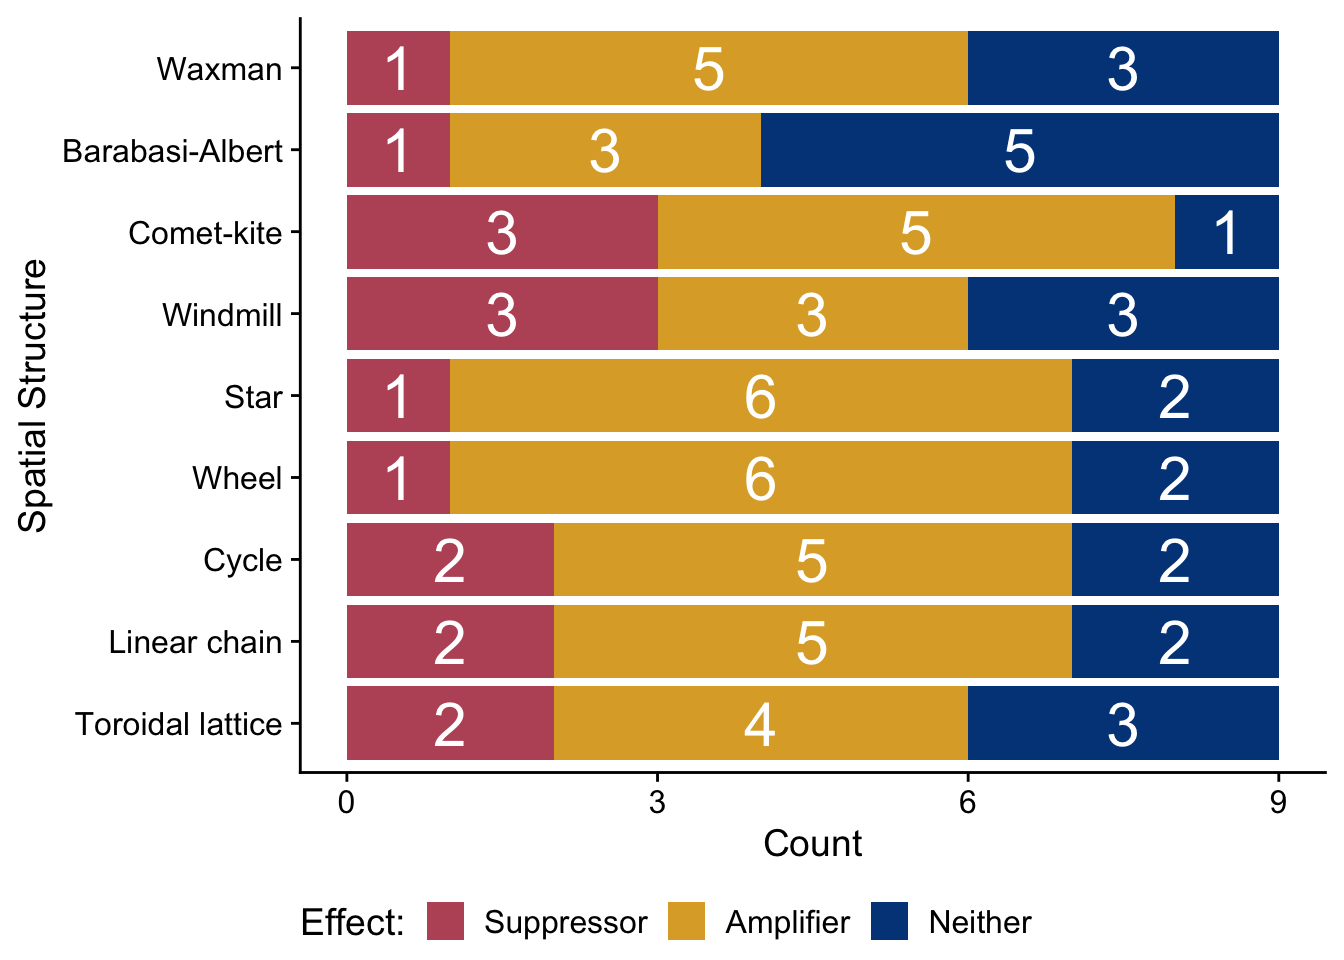
\includegraphics{supplemental-material_files/figure-latex/unnamed-chunk-17-1.pdf}

\hypertarget{graph-property-correlations}{%
\chapter{Graph property correlations}\label{graph-property-correlations}}

We screened for graph properties correlated with community transitionability scores.

\hypertarget{dependencies-and-setup-1}{%
\section{Dependencies and setup}\label{dependencies-and-setup-1}}

\begin{Shaded}
\begin{Highlighting}[]
\FunctionTok{library}\NormalTok{(tidyverse)}
\FunctionTok{library}\NormalTok{(Hmisc)}
\FunctionTok{library}\NormalTok{(broom)}
\FunctionTok{library}\NormalTok{(knitr)}
\FunctionTok{library}\NormalTok{(kableExtra)}
\end{Highlighting}
\end{Shaded}

\begin{Shaded}
\begin{Highlighting}[]
\CommentTok{\# Check if Rmd is being compiled using bookdown}
\NormalTok{bookdown }\OtherTok{\textless{}{-}} \FunctionTok{exists}\NormalTok{(}\StringTok{"bookdown\_build"}\NormalTok{)}
\end{Highlighting}
\end{Shaded}

\begin{Shaded}
\begin{Highlighting}[]
\NormalTok{experiment\_slug }\OtherTok{\textless{}{-}} \StringTok{"2024{-}03{-}08{-}varied{-}interaction{-}matrices"}
\NormalTok{working\_directory }\OtherTok{\textless{}{-}} \FunctionTok{paste}\NormalTok{(}
  \StringTok{"experiments"}\NormalTok{,}
\NormalTok{  experiment\_slug,}
  \StringTok{"analysis"}\NormalTok{,}
  \AttributeTok{sep =} \StringTok{"/"}
\NormalTok{)}
\CommentTok{\# Adjust working directory if being knitted for bookdown build.}
\ControlFlowTok{if}\NormalTok{ (bookdown) \{}
\NormalTok{  working\_directory }\OtherTok{\textless{}{-}} \FunctionTok{paste0}\NormalTok{(}
\NormalTok{    bookdown\_wd\_prefix,}
\NormalTok{    working\_directory}
\NormalTok{  )}
\NormalTok{\}}

\NormalTok{plot\_dir }\OtherTok{\textless{}{-}} \FunctionTok{paste}\NormalTok{(}
\NormalTok{  working\_directory,}
  \StringTok{"plots"}\NormalTok{,}
  \AttributeTok{sep =} \StringTok{"/"}
\NormalTok{)}

\NormalTok{data\_path }\OtherTok{\textless{}{-}} \FunctionTok{paste}\NormalTok{(}
\NormalTok{  working\_directory,}
  \StringTok{"data"}\NormalTok{,}
  \StringTok{"world\_summary\_final\_update\_with{-}graph{-}props.csv"}\NormalTok{,}
  \AttributeTok{sep =} \StringTok{"/"}
\NormalTok{)}
\NormalTok{data }\OtherTok{\textless{}{-}} \FunctionTok{read\_csv}\NormalTok{(data\_path)}
\end{Highlighting}
\end{Shaded}

Set cowplot theme as default plotting theme.

\begin{Shaded}
\begin{Highlighting}[]
\FunctionTok{theme\_set}\NormalTok{(}\FunctionTok{theme\_cowplot}\NormalTok{())}
\end{Highlighting}
\end{Shaded}

\hypertarget{data-preprocessing-1}{%
\section{Data preprocessing}\label{data-preprocessing-1}}

\begin{Shaded}
\begin{Highlighting}[]
\NormalTok{max\_update }\OtherTok{\textless{}{-}} \FunctionTok{max}\NormalTok{(data}\SpecialCharTok{$}\NormalTok{update)}
\CommentTok{\# Ensure that we just have measurements from final update.}
\NormalTok{data }\OtherTok{\textless{}{-}}\NormalTok{ data }\SpecialCharTok{\%\textgreater{}\%}
  \FunctionTok{filter}\NormalTok{(update }\SpecialCharTok{==}\NormalTok{ max\_update) }\SpecialCharTok{\%\textgreater{}\%}
  \FunctionTok{mutate}\NormalTok{(}
    \AttributeTok{interaction\_matrix =} \FunctionTok{as.factor}\NormalTok{(interaction\_matrix),}
    \AttributeTok{graph\_type =} \FunctionTok{as.factor}\NormalTok{(graph\_type),}
    \AttributeTok{summary\_mode =} \FunctionTok{as.factor}\NormalTok{(summary\_mode),}
    \AttributeTok{update =} \FunctionTok{as.numeric}\NormalTok{(update),}
    \AttributeTok{SEED =} \FunctionTok{as.factor}\NormalTok{(SEED),}
    \AttributeTok{graph\_file =} \FunctionTok{str\_split\_i}\NormalTok{(DIFFUSION\_SPATIAL\_STRUCTURE\_FILE, }\StringTok{"/"}\NormalTok{, }\SpecialCharTok{{-}}\DecValTok{1}\NormalTok{)}
\NormalTok{  ) }\SpecialCharTok{\%\textgreater{}\%}
  \FunctionTok{mutate}\NormalTok{(}
    \AttributeTok{graph\_file =} \FunctionTok{as.factor}\NormalTok{(graph\_file)}
\NormalTok{  )}
\CommentTok{\# write\_csv(}
\CommentTok{\#   data,}
\CommentTok{\#   "world\_summary\_final\_update.csv"}
\CommentTok{\# )}

\CommentTok{\# For each row, assign graph properties}
\NormalTok{properties }\OtherTok{\textless{}{-}} \FunctionTok{c}\NormalTok{(}
  \StringTok{"graph\_prop\_density"}\NormalTok{,}
  \StringTok{"graph\_prop\_degree\_mean"}\NormalTok{,}
  \StringTok{"graph\_prop\_degree\_median"}\NormalTok{,}
  \StringTok{"graph\_prop\_degree\_variance"}\NormalTok{,}
  \StringTok{"graph\_prop\_girth"}\NormalTok{,}
  \StringTok{"graph\_prop\_degree\_assortivity\_coef"}\NormalTok{,}
  \StringTok{"graph\_prop\_num\_bridges"}\NormalTok{,}
  \StringTok{"graph\_prop\_max\_clique\_size"}\NormalTok{,}
  \StringTok{"graph\_prop\_transitivity"}\NormalTok{,}
  \StringTok{"graph\_prop\_avg\_clustering"}\NormalTok{,}
  \StringTok{"graph\_prop\_num\_connected\_components"}\NormalTok{,}
  \StringTok{"graph\_prop\_num\_articulation\_points"}\NormalTok{,}
  \StringTok{"graph\_prop\_avg\_node\_connectivity"}\NormalTok{,}
  \StringTok{"graph\_prop\_edge\_connectivity"}\NormalTok{,}
  \StringTok{"graph\_prop\_node\_connectivity"}\NormalTok{,}
  \StringTok{"graph\_prop\_diameter"}\NormalTok{,}
  \StringTok{"graph\_prop\_radius"}\NormalTok{,}
  \StringTok{"graph\_prop\_kemeny\_constant"}\NormalTok{,}
  \StringTok{"graph\_prop\_global\_efficiency"}\NormalTok{,}
  \StringTok{"graph\_prop\_wiener\_index"}\NormalTok{,}
  \StringTok{"graph\_prop\_longest\_shortest\_path"}
\NormalTok{)}

\CommentTok{\# (3) Pivot longer}
\NormalTok{long\_data }\OtherTok{\textless{}{-}}\NormalTok{ data }\SpecialCharTok{\%\textgreater{}\%}
  \FunctionTok{mutate}\NormalTok{(}
    \AttributeTok{graph\_prop\_diameter =} \FunctionTok{case\_when}\NormalTok{(}
\NormalTok{      graph\_prop\_diameter }\SpecialCharTok{==} \StringTok{"error"} \SpecialCharTok{\textasciitilde{}} \StringTok{"{-}1"}\NormalTok{,}
      \AttributeTok{.default =}\NormalTok{ graph\_prop\_diameter}
\NormalTok{    ),}
    \AttributeTok{graph\_prop\_radius =} \FunctionTok{case\_when}\NormalTok{(}
\NormalTok{      graph\_prop\_radius }\SpecialCharTok{==} \StringTok{"error"} \SpecialCharTok{\textasciitilde{}} \StringTok{"{-}1"}\NormalTok{,}
      \AttributeTok{.default =}\NormalTok{ graph\_prop\_radius}
\NormalTok{    ),}
    \AttributeTok{graph\_prop\_kemeny\_constant =} \FunctionTok{case\_when}\NormalTok{(}
\NormalTok{      graph\_prop\_kemeny\_constant }\SpecialCharTok{==} \StringTok{"error"} \SpecialCharTok{\textasciitilde{}} \StringTok{"{-}1"}\NormalTok{,}
      \AttributeTok{.default =}\NormalTok{ graph\_prop\_kemeny\_constant}
\NormalTok{    )}
\NormalTok{  ) }\SpecialCharTok{\%\textgreater{}\%}
  \FunctionTok{mutate}\NormalTok{(}
    \AttributeTok{graph\_prop\_diameter =} \FunctionTok{as.numeric}\NormalTok{(graph\_prop\_diameter),}
    \AttributeTok{graph\_prop\_radius =} \FunctionTok{as.numeric}\NormalTok{(graph\_prop\_radius),}
    \AttributeTok{graph\_prop\_kemeny\_constant =} \FunctionTok{as.numeric}\NormalTok{(graph\_prop\_kemeny\_constant)}
\NormalTok{  ) }\SpecialCharTok{\%\textgreater{}\%}
  \FunctionTok{select}\NormalTok{(}
    \SpecialCharTok{!}\FunctionTok{c}\NormalTok{(}
\NormalTok{      DIFFUSION\_SPATIAL\_STRUCTURE\_FILE,}
\NormalTok{      GROUP\_REPRO\_SPATIAL\_STRUCTURE\_FILE,}
\NormalTok{      INTERACTION\_SOURCE}
\NormalTok{    )}
\NormalTok{  ) }\SpecialCharTok{\%\textgreater{}\%}
  \FunctionTok{filter}\NormalTok{(}
\NormalTok{    summary\_mode }\SpecialCharTok{==} \StringTok{"ranked\_threshold"}
\NormalTok{  ) }\SpecialCharTok{\%\textgreater{}\%}
  \FunctionTok{pivot\_longer}\NormalTok{(}
    \AttributeTok{cols =}\NormalTok{ properties,}
    \AttributeTok{names\_to =} \StringTok{"graph\_property"}\NormalTok{,}
    \AttributeTok{values\_to =} \StringTok{"graph\_property\_value"}
\NormalTok{  ) }\SpecialCharTok{\%\textgreater{}\%}
  \FunctionTok{filter}\NormalTok{(}
\NormalTok{    (}\SpecialCharTok{!}\FunctionTok{is.na}\NormalTok{(graph\_property\_value)) }\SpecialCharTok{\&}\NormalTok{ graph\_property\_value }\SpecialCharTok{!=} \StringTok{"Inf"} \SpecialCharTok{\&}
\NormalTok{    (}\SpecialCharTok{!}\NormalTok{(graph\_property }\SpecialCharTok{==} \StringTok{"graph\_prop\_diameter"} \SpecialCharTok{\&}\NormalTok{ (graph\_property\_value }\SpecialCharTok{==} \StringTok{"{-}1"}\NormalTok{))) }\SpecialCharTok{\&}
\NormalTok{    (}\SpecialCharTok{!}\NormalTok{(graph\_property }\SpecialCharTok{==} \StringTok{"graph\_prop\_radius"} \SpecialCharTok{\&}\NormalTok{ (graph\_property\_value }\SpecialCharTok{==} \StringTok{"{-}1"}\NormalTok{))) }\SpecialCharTok{\&}
\NormalTok{    (}\SpecialCharTok{!}\NormalTok{(graph\_property }\SpecialCharTok{==} \StringTok{"graph\_prop\_kemeny\_constant"} \SpecialCharTok{\&}\NormalTok{ (graph\_property\_value }\SpecialCharTok{==} \StringTok{"{-}1"}\NormalTok{)))}
\NormalTok{  ) }\SpecialCharTok{\%\textgreater{}\%}
  \FunctionTok{mutate}\NormalTok{(}
    \AttributeTok{graph\_property\_value =} \FunctionTok{as.numeric}\NormalTok{(graph\_property\_value),}
    \AttributeTok{graph\_property =} \FunctionTok{str\_remove}\NormalTok{(graph\_property, }\StringTok{"graph\_prop\_"}\NormalTok{)}
\NormalTok{  ) }\SpecialCharTok{\%\textgreater{}\%}
  \FunctionTok{mutate}\NormalTok{(}
    \AttributeTok{graph\_property =} \FunctionTok{as.factor}\NormalTok{(graph\_property)}
\NormalTok{  )}
\CommentTok{\# write\_csv(long\_data, "test.csv")}
\end{Highlighting}
\end{Shaded}

\hypertarget{plot-relationships-between-transitionability-and-graph-properties}{%
\section{Plot relationships between transitionability and graph properties}\label{plot-relationships-between-transitionability-and-graph-properties}}

\begin{Shaded}
\begin{Highlighting}[]
\NormalTok{rel\_plot }\OtherTok{\textless{}{-}}\NormalTok{ long\_data }\SpecialCharTok{\%\textgreater{}\%}
  \FunctionTok{ggplot}\NormalTok{(}
    \FunctionTok{aes}\NormalTok{(}
      \AttributeTok{x =}\NormalTok{ graph\_property\_value,}
      \AttributeTok{y =}\NormalTok{ logged\_mult\_score}
\NormalTok{    )}
\NormalTok{  ) }\SpecialCharTok{+}
  \FunctionTok{geom\_point}\NormalTok{(}\FunctionTok{aes}\NormalTok{(}\AttributeTok{color =}\NormalTok{ graph\_type)) }\SpecialCharTok{+}
  \FunctionTok{geom\_smooth}\NormalTok{(}
    \AttributeTok{method =} \StringTok{"lm"}\NormalTok{,}
    \AttributeTok{color =} \StringTok{"black"}
\NormalTok{  ) }\SpecialCharTok{+}
  \FunctionTok{facet\_grid}\NormalTok{(}
\NormalTok{    interaction\_matrix }\SpecialCharTok{\textasciitilde{}}\NormalTok{ graph\_property,}
    \AttributeTok{scales =} \StringTok{"free"}
\NormalTok{  )}

\NormalTok{rel\_plot}
\end{Highlighting}
\end{Shaded}

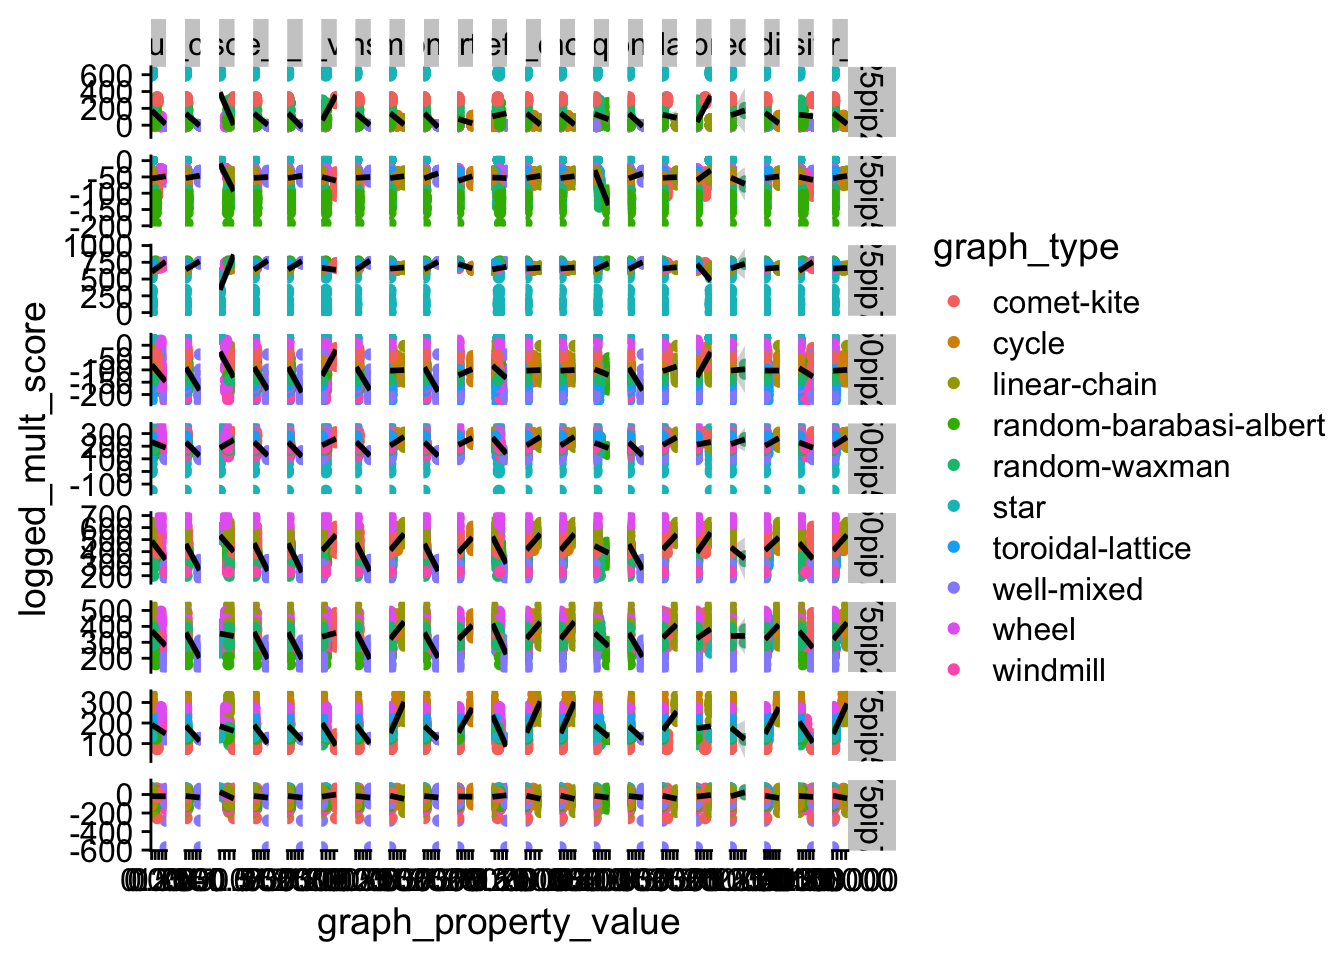
\includegraphics{supplemental-material_files/figure-latex/unnamed-chunk-23-1.pdf}

\begin{Shaded}
\begin{Highlighting}[]
\FunctionTok{ggsave}\NormalTok{(}
  \AttributeTok{plot =}\NormalTok{ rel\_plot,}
  \AttributeTok{filename =} \FunctionTok{paste}\NormalTok{(}
\NormalTok{    plot\_dir,}
    \StringTok{"property\_relationships.pdf"}\NormalTok{,}
    \AttributeTok{sep =} \StringTok{"/"}
\NormalTok{  ),}
  \AttributeTok{width =} \DecValTok{40}\NormalTok{,}
  \AttributeTok{height =} \DecValTok{20}
\NormalTok{)}
\end{Highlighting}
\end{Shaded}

\hypertarget{measure-correlations}{%
\section{Measure correlations}\label{measure-correlations}}

\begin{Shaded}
\begin{Highlighting}[]
\CommentTok{\# Reference for running correlations over tidy data:}
\CommentTok{\# https://dominicroye.github.io/en/2019/tidy{-}correlation{-}tests{-}in{-}r/}
\NormalTok{cor\_fun }\OtherTok{\textless{}{-}} \ControlFlowTok{function}\NormalTok{(data) \{}
  \FunctionTok{cor.test}\NormalTok{(}
\NormalTok{    data}\SpecialCharTok{$}\NormalTok{graph\_property\_value,}
\NormalTok{    data}\SpecialCharTok{$}\NormalTok{logged\_mult\_score,}
    \AttributeTok{method =} \StringTok{"spearman"}\NormalTok{,}
    \AttributeTok{exact =} \ConstantTok{FALSE}
\NormalTok{  ) }\SpecialCharTok{\%\textgreater{}\%} \FunctionTok{tidy}\NormalTok{()}
\NormalTok{\}}

\NormalTok{nested }\OtherTok{\textless{}{-}}\NormalTok{ long\_data }\SpecialCharTok{\%\textgreater{}\%}
  \FunctionTok{select}\NormalTok{(}
    \FunctionTok{c}\NormalTok{(}
\NormalTok{      interaction\_matrix,}
\NormalTok{      graph\_property,}
\NormalTok{      graph\_property\_value,}
\NormalTok{      logged\_mult\_score}
\NormalTok{    )}
\NormalTok{  ) }\SpecialCharTok{\%\textgreater{}\%}
  \FunctionTok{group\_by}\NormalTok{(interaction\_matrix, graph\_property) }\SpecialCharTok{\%\textgreater{}\%}
  \FunctionTok{nest}\NormalTok{() }\SpecialCharTok{\%\textgreater{}\%}
  \FunctionTok{mutate}\NormalTok{(}
    \AttributeTok{model =} \FunctionTok{map}\NormalTok{(data, cor\_fun)}
\NormalTok{  )}

\NormalTok{full\_corr }\OtherTok{\textless{}{-}} \FunctionTok{select}\NormalTok{(nested, }\SpecialCharTok{{-}}\NormalTok{data) }\SpecialCharTok{\%\textgreater{}\%} \FunctionTok{unnest}\NormalTok{()}
\NormalTok{full\_corr }\OtherTok{\textless{}{-}}\NormalTok{ full\_corr }\SpecialCharTok{\%\textgreater{}\%}
  \FunctionTok{mutate}\NormalTok{(}
    \AttributeTok{abs\_estimate =} \FunctionTok{abs}\NormalTok{(estimate)}
\NormalTok{  ) }\SpecialCharTok{\%\textgreater{}\%}
  \FunctionTok{arrange}\NormalTok{(}
    \FunctionTok{desc}\NormalTok{(abs\_estimate)}
\NormalTok{  ) }\SpecialCharTok{\%\textgreater{}\%}
  \FunctionTok{group\_by}\NormalTok{(}
\NormalTok{    interaction\_matrix}
\NormalTok{  ) }\SpecialCharTok{\%\textgreater{}\%}
  \FunctionTok{mutate}\NormalTok{(}
    \AttributeTok{p.value.adj =} \FunctionTok{p.adjust}\NormalTok{(p.value, }\AttributeTok{method =} \StringTok{"holm"}\NormalTok{)}
\NormalTok{  ) }\SpecialCharTok{\%\textgreater{}\%}
  \FunctionTok{filter}\NormalTok{(}
\NormalTok{    p.value.adj }\SpecialCharTok{\textless{}=} \FloatTok{0.05}
\NormalTok{  )}

\NormalTok{full\_corr\_table }\OtherTok{\textless{}{-}} \FunctionTok{kable}\NormalTok{(full\_corr) }\SpecialCharTok{\%\textgreater{}\%}
  \FunctionTok{kable\_styling}\NormalTok{(}\AttributeTok{latex\_options =} \StringTok{"striped"}\NormalTok{)}
\FunctionTok{save\_kable}\NormalTok{(}
\NormalTok{  full\_corr\_table,}
  \FunctionTok{paste}\NormalTok{(}
\NormalTok{    plot\_dir,}
    \StringTok{"correlation\_table.pdf"}\NormalTok{,}
    \AttributeTok{sep =} \StringTok{"/"}
\NormalTok{  )}
\NormalTok{)}
\end{Highlighting}
\end{Shaded}

\hypertarget{top-three-significant-correlations-per-interaction-matrix}{%
\subsection{Top three significant correlations per interaction matrix}\label{top-three-significant-correlations-per-interaction-matrix}}

Break correlations down by interaction matrix

\begin{Shaded}
\begin{Highlighting}[]
\NormalTok{interaction\_matrices }\OtherTok{\textless{}{-}} \FunctionTok{levels}\NormalTok{(long\_data}\SpecialCharTok{$}\NormalTok{interaction\_matrix)}

\ControlFlowTok{for}\NormalTok{ (mat\_type }\ControlFlowTok{in}\NormalTok{ interaction\_matrices) \{}
\NormalTok{  mat\_data }\OtherTok{\textless{}{-}} \FunctionTok{filter}\NormalTok{(long\_data, interaction\_matrix }\SpecialCharTok{==}\NormalTok{ mat\_type)}

\NormalTok{  nested }\OtherTok{\textless{}{-}}\NormalTok{ mat\_data }\SpecialCharTok{\%\textgreater{}\%}
    \FunctionTok{select}\NormalTok{(}
      \FunctionTok{c}\NormalTok{(}
\NormalTok{        interaction\_matrix,}
\NormalTok{        graph\_property,}
\NormalTok{        graph\_property\_value,}
\NormalTok{        logged\_mult\_score}
\NormalTok{      )}
\NormalTok{    ) }\SpecialCharTok{\%\textgreater{}\%}
    \FunctionTok{group\_by}\NormalTok{(interaction\_matrix, graph\_property) }\SpecialCharTok{\%\textgreater{}\%}
    \FunctionTok{nest}\NormalTok{() }\SpecialCharTok{\%\textgreater{}\%}
    \FunctionTok{mutate}\NormalTok{(}
      \AttributeTok{model =} \FunctionTok{map}\NormalTok{(data, cor\_fun)}
\NormalTok{    )}

\NormalTok{  im\_corr }\OtherTok{\textless{}{-}} \FunctionTok{select}\NormalTok{(nested, }\SpecialCharTok{{-}}\NormalTok{data) }\SpecialCharTok{\%\textgreater{}\%} \FunctionTok{unnest}\NormalTok{()}
\NormalTok{  im\_corr }\OtherTok{\textless{}{-}}\NormalTok{ im\_corr }\SpecialCharTok{\%\textgreater{}\%}
    \FunctionTok{mutate}\NormalTok{(}
      \AttributeTok{abs\_estimate =} \FunctionTok{abs}\NormalTok{(estimate)}
\NormalTok{    ) }\SpecialCharTok{\%\textgreater{}\%}
    \FunctionTok{arrange}\NormalTok{(}
      \FunctionTok{desc}\NormalTok{(abs\_estimate)}
\NormalTok{    ) }\SpecialCharTok{\%\textgreater{}\%}
    \FunctionTok{ungroup}\NormalTok{() }\SpecialCharTok{\%\textgreater{}\%}
    \FunctionTok{group\_by}\NormalTok{(}
\NormalTok{      interaction\_matrix}
\NormalTok{    ) }\SpecialCharTok{\%\textgreater{}\%}
    \FunctionTok{mutate}\NormalTok{(}
      \AttributeTok{p.value.adj =} \FunctionTok{p.adjust}\NormalTok{(p.value, }\AttributeTok{method =} \StringTok{"holm"}\NormalTok{)}
\NormalTok{    ) }\SpecialCharTok{\%\textgreater{}\%}
    \FunctionTok{filter}\NormalTok{(}
\NormalTok{      p.value.adj }\SpecialCharTok{\textless{}} \FloatTok{0.05}
\NormalTok{    )}

\NormalTok{  im\_corr\_table }\OtherTok{\textless{}{-}} \FunctionTok{kable}\NormalTok{(im\_corr) }\SpecialCharTok{\%\textgreater{}\%}
    \FunctionTok{kable\_styling}\NormalTok{(}\AttributeTok{latex\_options =} \StringTok{"striped"}\NormalTok{)}
  \FunctionTok{save\_kable}\NormalTok{(}
\NormalTok{    im\_corr\_table,}
    \FunctionTok{paste}\NormalTok{(}
\NormalTok{      plot\_dir,}
      \FunctionTok{paste0}\NormalTok{(}\StringTok{"correlation\_table\_"}\NormalTok{, mat\_type, }\StringTok{".pdf"}\NormalTok{),}
      \AttributeTok{sep =} \StringTok{"/"}
\NormalTok{    )}
\NormalTok{  )}

\NormalTok{  top\_corr }\OtherTok{\textless{}{-}}\NormalTok{ im\_corr }\SpecialCharTok{\%\textgreater{}\%}
    \FunctionTok{slice\_max}\NormalTok{(}
\NormalTok{      abs\_estimate,}
      \AttributeTok{n =} \DecValTok{3}
\NormalTok{    )}
\NormalTok{  top\_corr\_table }\OtherTok{\textless{}{-}} \FunctionTok{kable}\NormalTok{(top\_corr) }\SpecialCharTok{\%\textgreater{}\%}
    \FunctionTok{kable\_styling}\NormalTok{(}\AttributeTok{latex\_options =} \StringTok{"striped"}\NormalTok{)}

  \FunctionTok{save\_kable}\NormalTok{(}
\NormalTok{    top\_corr\_table,}
    \FunctionTok{paste}\NormalTok{(}
\NormalTok{      plot\_dir,}
      \FunctionTok{paste0}\NormalTok{(}\StringTok{"t3\_correlation\_table\_"}\NormalTok{, mat\_type, }\StringTok{".pdf"}\NormalTok{),}
      \AttributeTok{sep =} \StringTok{"/"}
\NormalTok{    )}
\NormalTok{  )}

\NormalTok{\}}
\end{Highlighting}
\end{Shaded}

\hypertarget{distrubition-of-correlations-0.5-strength}{%
\subsection{Distrubition of correlations \textgreater= 0.5 strength}\label{distrubition-of-correlations-0.5-strength}}

\begin{Shaded}
\begin{Highlighting}[]
\CommentTok{\# Look at distribution of correlations \textgreater{}= 0.5 strength}
\NormalTok{corr\_str\_thresh }\OtherTok{\textless{}{-}} \FloatTok{0.5}
\NormalTok{full\_corr\_thresh }\OtherTok{\textless{}{-}}\NormalTok{ full\_corr }\SpecialCharTok{\%\textgreater{}\%}
  \FunctionTok{mutate}\NormalTok{(}
    \AttributeTok{direction =} \FunctionTok{case\_when}\NormalTok{(}
\NormalTok{      estimate }\SpecialCharTok{\textless{}} \DecValTok{0} \SpecialCharTok{\textasciitilde{}} \StringTok{"Negative"}\NormalTok{,}
\NormalTok{      estimate }\SpecialCharTok{\textgreater{}=} \DecValTok{0} \SpecialCharTok{\textasciitilde{}} \StringTok{"Positive"}
\NormalTok{    )}
\NormalTok{  ) }\SpecialCharTok{\%\textgreater{}\%}
  \FunctionTok{mutate}\NormalTok{(}
    \AttributeTok{direction =} \FunctionTok{as.factor}\NormalTok{(direction)}
\NormalTok{  ) }\SpecialCharTok{\%\textgreater{}\%}
  \FunctionTok{filter}\NormalTok{(abs\_estimate }\SpecialCharTok{\textgreater{}=}\NormalTok{ corr\_str\_thresh }\SpecialCharTok{\&}\NormalTok{ p.value.adj }\SpecialCharTok{\textless{}=} \FloatTok{0.05}\NormalTok{)}

\NormalTok{corr\_counts }\OtherTok{\textless{}{-}}\NormalTok{ full\_corr\_thresh }\SpecialCharTok{\%\textgreater{}\%}
\NormalTok{  dplyr}\SpecialCharTok{::}\FunctionTok{group\_by}\NormalTok{(graph\_property, direction) }\SpecialCharTok{\%\textgreater{}\%}
\NormalTok{  dplyr}\SpecialCharTok{::}\FunctionTok{summarize}\NormalTok{(}
    \AttributeTok{n =} \FunctionTok{n}\NormalTok{()}
\NormalTok{  )}

\CommentTok{\# If something has one direction, but not other, fill in 0 for other.}
\CommentTok{\# For property in properties}
\NormalTok{correlation\_dirs\_plot }\OtherTok{\textless{}{-}}\NormalTok{ corr\_counts }\SpecialCharTok{\%\textgreater{}\%}
  \FunctionTok{ggplot}\NormalTok{(}
    \FunctionTok{aes}\NormalTok{(}
      \AttributeTok{x =}\NormalTok{ graph\_property,}
      \AttributeTok{fill =}\NormalTok{ direction,}
      \AttributeTok{y =}\NormalTok{ n}
\NormalTok{    )}
\NormalTok{  ) }\SpecialCharTok{+}
  \FunctionTok{geom\_bar}\NormalTok{(}\AttributeTok{stat =} \StringTok{"identity"}\NormalTok{, }\AttributeTok{position =} \FunctionTok{position\_dodge}\NormalTok{(), }\AttributeTok{alpha =} \FloatTok{0.75}\NormalTok{) }\SpecialCharTok{+}
  \FunctionTok{coord\_flip}\NormalTok{()}

\FunctionTok{ggsave}\NormalTok{(}
  \AttributeTok{plot =}\NormalTok{ correlation\_dirs\_plot,}
  \AttributeTok{filename =} \FunctionTok{paste}\NormalTok{(}
\NormalTok{    plot\_dir,}
    \StringTok{"most\_moderate\_correlations.pdf"}\NormalTok{,}
    \AttributeTok{sep =} \StringTok{"/"}
\NormalTok{  )}
\NormalTok{)}
\NormalTok{correlation\_dirs\_plot}
\end{Highlighting}
\end{Shaded}

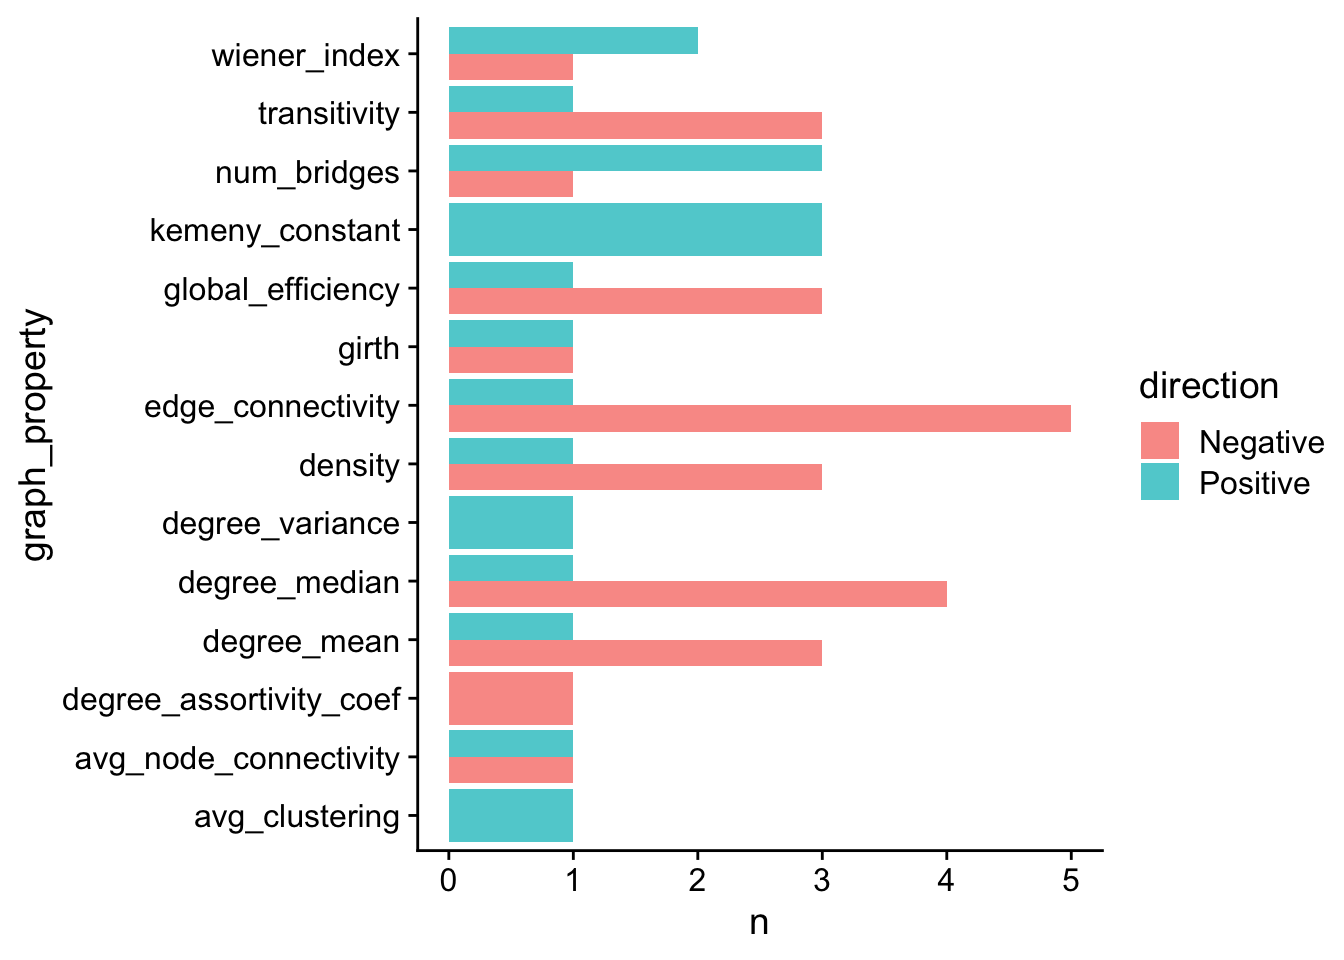
\includegraphics{supplemental-material_files/figure-latex/unnamed-chunk-26-1.pdf}

  \bibliography{packages.bib,supplemental.bib}

\end{document}
